%%%%%%%%%%%%%%%%%%%%%%%%%%%%%%%%%%%%%%%%%
% Short Sectioned Assignment LaTeX Template Version 1.0 (5/5/12)
% This template has been downloaded from: http://www.LaTeXTemplates.com
% Original author:  Frits Wenneker (http://www.howtotex.com)
% License: CC BY-NC-SA 3.0 (http://creativecommons.org/licenses/by-nc-sa/3.0/)
%%%%%%%%%%%%%%%%%%%%%%%%%%%%%%%%%%%%%%%%%

% \documentclass[paper=a4, fontsize=11pt]{scrartcl} % A4 paper and 11pt font size
\documentclass[12pt, a4paper, openany]{book}
\usepackage[T1]{fontenc} % Use 8-bit encoding that has 256 glyphs
\usepackage{fourier} % Use the Adobe Utopia font for the document - comment this line to return to the LaTeX default
\usepackage[utf8]{inputenc}
\usepackage{listings} % para insertar código con formato similar al editor
\usepackage[spanish, es-tabla]{babel} % Selecciona el español para palabras introducidas automáticamente, p.ej. "septiembre" en la fecha y especifica que se use la palabra Tabla en vez de Cuadro
\usepackage{url} % ,href} %para incluir URLs e hipervínculos dentro del texto (aunque hay que instalar href)
\usepackage{graphics,graphicx, float} %para incluir imágenes y colocarlas
\usepackage[gen]{eurosym} %para incluir el símbolo del euro
\usepackage{cite} %para incluir citas del archivo <nombre>.bib
\usepackage{enumerate}
\usepackage{hyperref}
\usepackage{graphicx,subfig}
\usepackage{tabularx, multirow}
\usepackage{booktabs}
\usepackage[table,xcdraw]{xcolor}
\newcommand{\tabitem}{~~\llap{\textbullet}~~}

\hypersetup{
	colorlinks=true,	% false: boxed links; true: colored links
	linkcolor=black,	% color of internal links
	urlcolor=cyan		% color of external links
}
%\renewcommand{\familydefault}{\sfdefault}
\usepackage{fancyhdr} % Custom headers and footers
\pagestyle{fancyplain} % Makes all pages in the document conform to the custom headers and footers
\fancyhead[EL]{Asistente de Voz Modular usando APIs libres} % Empty left header
\fancyhead[ER]{} % Empty left header
\fancyhead[C]{} % Empty center header
\fancyhead[OL]{} % My name
\fancyhead[OR]{Iván Valero Rodríguez} % My name
\fancyfoot[L]{} % Empty left footer
\fancyfoot[C]{} % Empty center footer
\fancyfoot[R]{\thepage} % Page numbering for right footer
%\renewcommand{\headrulewidth}{0pt} % Remove header underlines
\renewcommand{\footrulewidth}{0pt} % Remove footer underlines
\setlength{\headheight}{13.6pt} % Customize the height of the header

\usepackage{titlesec, blindtext, color}
\definecolor{gray75}{gray}{0.75}
\definecolor{azul}{HTML}{456CF7}
\definecolor{lightblue}{HTML}{d5d9e6}
\definecolor{mintgreen}{HTML}{c2edc5}
\newcommand{\hsp}{\hspace{20pt}}
\setcounter{secnumdepth}{4}
\usepackage[Bjornstrup]{fncychap}
\ChNumVar{\fontsize{76}{80}\usefont{OT1}{pzc}{m}{n}\selectfont}
\ChTitleVar{\raggedleft\Large\bfseries}

\renewcommand\DOCH{%
  \settowidth{\py}{\CNoV\thechapter}
  \addtolength{\py}{-10pt}
  \fboxsep=0pt%
  \colorbox{lightblue}{\rule{0pt}{40pt}\parbox[b]{\textwidth}{\hfill}}%
  \kern-\py\raise20pt%
  \hbox{\color{azul}\CNoV\thechapter}\\%
}

\renewcommand\DOTI[1]{%
  \nointerlineskip\raggedright%
  \fboxsep=\myhi%
  \vskip-1ex%
  \colorbox{lightblue}{\parbox[t]{\mylen}{\CTV\FmTi{#1}}}\par\nobreak%
  \vskip 40pt%
}

\renewcommand\DOTIS[1]{%
  \fboxsep=0pt
  \colorbox{mintgreen}{\rule{0pt}{40pt}\parbox[b]{\textwidth}{\hfill}}\\%
  \nointerlineskip\raggedright%
  \fboxsep=\myhi%
  \colorbox{mintgreen}{\parbox[t]{\mylen}{\CTV\FmTi{#1}}}\par\nobreak%
  \vskip 40pt%
 }



\begin{document}

	% Plantilla portada UGR
	\begin{titlepage}
\newlength{\centeroffset}
\setlength{\centeroffset}{-0.5\oddsidemargin}
\addtolength{\centeroffset}{0.5\evensidemargin}
\thispagestyle{empty}

\noindent\hspace*{\centeroffset}\begin{minipage}{\textwidth}

\centering

\includegraphics[width=0.9\textwidth]{logos/logo_ugr.jpg}\\[1.4cm]

\textsc{ \Large TRABAJO FIN DE GRADO\\[0.2cm]}
\textsc{ GRADO EN INGENIERÍA INFORMÁTICA}\\[1cm]

{\Huge\bfseries Asistente de voz modular \\}
\noindent\rule[-1ex]{\textwidth}{3pt}\\[3.5ex]
{\large\bfseries usando APIs libres }
\end{minipage}

\vspace{2.5cm}
\noindent\hspace*{\centeroffset}
\begin{minipage}{\textwidth}
\centering

\textbf{Autor}\\ {Iván Valero Rodríguez}\\[2.5ex]
\textbf{Director}\\ {Pablo García Sánchez}\\[2cm]

\includegraphics[width=0.3\textwidth]{logos/etsiit_logo.png}\\[0.1cm]
\textsc{Escuela Técnica Superior de Ingenierías Informática y de Telecomunicación}\\
\textsc{---}\\
Granada, Julio de 2021
\end{minipage}
\end{titlepage}


	% Plantilla prefacio UGR
	\thispagestyle{empty}

\begin{center}
{\large\bfseries Título \\ Subtítulo }\\
\end{center}
\begin{center}
Nombre Del Estudiante\\
\end{center}

%\vspace{0.7cm}

\vspace{0.5cm}
\noindent{\textbf{Palabras clave}: \textit{software libre}
\vspace{0.7cm}

\noindent{\textbf{Resumen}\\
	

\cleardoublepage

\begin{center}
	{\large\bfseries Same, but in English}\\
\end{center}
\begin{center}
	Student's name\\
\end{center}
\vspace{0.5cm}
\noindent{\textbf{Keywords}: \textit{open source}, \textit{floss}
\vspace{0.7cm}

\noindent{\textbf{Abstract}\\


\cleardoublepage

\thispagestyle{empty}

\noindent\rule[-1ex]{\textwidth}{2pt}\\[4.5ex]

D. \textbf{Tutora/e(s)}, Profesor(a) del ...

\vspace{0.5cm}

\textbf{Informo:}

\vspace{0.5cm}

Que el presente trabajo, titulado \textit{\textbf{Chief}},
ha sido realizado bajo mi supervisión por \textbf{Estudiante}, y autorizo la defensa de dicho trabajo ante el tribunal
que corresponda.

\vspace{0.5cm}

Y para que conste, expiden y firman el presente informe en Granada a Junio de 2018.

\vspace{1cm}

\textbf{El/la director(a)/es: }

\vspace{5cm}

\noindent \textbf{(nombre completo tutor/a/es)}

\chapter*{Agradecimientos}






	% Índice de contenidos
	\newpage
	\tableofcontents

	% Índice de imágenes y tablas
	\newpage
	\listoffigures

	% Si hay suficientes se incluirá dicho índice
	\listoftables 
	\newpage

	% Introducción
	\newpage 
	\chapter{Introducción}

\noindent\fbox{
	\parbox{\textwidth}{
		En esta sección se introducirá los conceptos que se irán desarrollando en el transcurso de este Trabajo Fin de Grado de cara a la definición del problema que se resolverá al realizar el proyecto. Hablaremos de la situación actual y qué puede aportar la temática de este proyecto a ésta.
	}
}

\section{Motivación}

\subsection{La sociedad de la Información y los Asistentes de Voz}
Hoy en día, la Sociedad de la Información está siendo un tema que integramos cada día más en nuestra vida. Desde la introducción de tecnologías como la computación y la telefonía, estos se han ido adaptando a entornos cada vez más generales. 

Actualmente, nuestro día a día está rodeado de sistemas software que gestionan la información relativa a nuestra persona en ámbitos como las administraciones públicas, entornos bancarios e incluso subimos historias en las redes sociales habiendo así, y aún intentando reservarse lo máximo posible, un esquema más o menos complejo de cada persona por las redes.

Además, cada tanto tiempo se publican piezas de \textit{hardware} o programas \textit{software} novedosos que se integran aún más en la vida cotidiana. Como ejemplos podemos tener innovaciones como los teléfonos móviles (quienes evolucionaron en los actuales \textit{smartphones}), los televisores que actualmente disponen de integraciones con los servicios de \textit{streaming}, y lo que en nuestro caso nos compete, que serían los asistentes de voz.

Los asistentes de voz se tratan de sistemas \textit{software} que pueden estar bien como aplicación para sistemas de escritorio, móviles o por Internet; o embebidos en un dispositivo \textit{hardware} que se sitúa en algún punto de la casa; con las cuales se interactúa con la voz, de forma que al hablarle al dispositivo se abra un proceso internamente que toma lo que se habla y devuelve generalmente la reproducción de un audio. Puede ser un sonido, una canción o una voz sintetizada respondiendo a la petición. 

Los Asistentes de Voz permiten una nueva dimensión en el mundo de los Dispositivos de Interfaz Humana, ya que en los últimos años la comunicación por voz está siendo habitual en aplicaciones de mensajería y el hecho de no necesitar usar casi las manos o la vista para interactuar con éstos podría hacer que sea de ayuda a personas con diversidad cognitiva o motora (por ejemplo, las personas ciegas, según discuten en  \cite{va-benefits}, donde se analizan varios supuestos y cómo los Asistentes de Voz podrían ayudar).

Además, depende de cómo se defina el tono del Asistente, se puede permitir una interacción más cercana a una conversación entre seres humanos.El hecho de que se quiera hacer esto último abre varias cuestiones, como saber qué temas hablar, en qué idiomas se podría comunicar o qué vocabulario usar.

Esto, por consecuencia, debería dar a una serie de patrones que debe seguir. Estos patrones pueden compartir una respuesta común o que un patrón pueda dar varias respuestas. Por consiguiente, uno de los posibles puntos a tratar sería cómo podemos hacer que esa información se pueda completar para que el léxico, habilidades y conocimientos de nuestro agente pueda enriquecerse.

Trataremos de definir más a detalle las acciones y entresijos que el sistema realiza (desde que recibe el audio hasta que da una respuesta) en el estado del arte.

\subsection{El desarrollo del \textit{Software} y la propiedad del código }
\subsubsection{Desarrollando Software}
Haciendo mención al profesor Alberto Espinosa \cite{Prieto2006-ss}, podríamos entender el software no sólo como aquellos programas que se pueden ejecutar en un computador, sino además a todo lo que lo relaciona, desde las metodologías empleadas en su desarrollo, los datos que internamente interpretan y cómo los organizan, el análisis de cómo se implementará el sistema resultante y, en general, toda herramienta que permita su realización. 

El proceso de hacer Software ha ido cambiando con el pasar de los años con tal de hacer más eficiente el proceso de diseño y codificación de este. Se pasó de un procedimiento lineal en cascada con una codificación sin estandarizar, a una serie de aproximaciones que todos los desarrolladores adoptan; basadas en estilos de codificación, metodologías ágiles como Scrum y XP, o patrones de diseño y arquitecturales; entre otros. 

Por consiguiente, se lleva a una comprensión del código y de cómo integrar el sistema o interactuar con éste, una documentación sobre todo lo que se haya implicado con tal de converger en el producto resultante.

Por lo que se ha expuesto entonces en este epígrafe, vemos que al trabajar en el área del Desarrollo del Software trabajamos con convenciones estandarizadas que acaban en una serie de documentos que exponen cómo se ha ideado el programa o programas a programar junto con instrucciones para poder compilarlo y/o instalarlo; el código ya programado (en general con comentarios) y el ejecutable o sistema montado (si se aplica)

\subsubsection{Las empresas y la propiedad del código}
Las empresas llevan adaptándose o adelantándose a los hábitos que la sociedad va experimentando día a día.
Desde la introducción de los computadores (primero en el ámbito científico y con el pasar de los años extendiéndose a un público más general), las empresas requieren de programas que por les faciliten la gestión y/o automatización de algunos ámbitos y procesos que aplican entre sus operaciones y responsabilidades.

Por consecuencia, se da una necesidad de preparar más programas para las terminales que satisfagan las tareas más mecánicas y repetitivas o que sirvan de ayuda a la realización de tal tarea consiguiendo más eficiencia en el proceso. Para suplir esa demanda se crean otros tipos de empresa dedicados a desarrollar ese software (a medida o para un grupo de usuarios más extendido) consiguiendo de paso algún beneficio económico. Entre ellos podríamos destacar a Microsoft, Apple o IBM, quienes en los últimos años han ido tomando relevancia en conjunto con la historia reciente de la computación y de la llegada del ordenador personal.

Eso sí, si estas empresas toman tiempo y recursos en realizar soluciones computacionales para satisfacer esas demandas con tal de conseguir beneficios, ¿cómo pueden protegerse de que la competencia pueda sacar fácilmente una versión con las mismas o similares prestaciones, sacando así una versión de esa solución por un precio menor? Una de las ideas más intuitivas sería simplemente \textbf{no dando el código} ni las instrucciones para montarlo, dando en su lugar sólo un ejecutable y las dependencias necesarias de forma que pueda correr en el Sistema Operativo (o varios de esos ejecutables si se han compilado versiones para diferentes arquitecturas y kernels, y si así se permite). 

Además, al hacer tal protección, según las leyes españolas, posee dos tipos de derechos \cite{propint-1996}:

\begin{itemize}
	\item \textbf{Derechos morales} Son aquellos derechos inalienables e irrenunciables por los que puede decidir sobre el objeto que se ha querido proteger legalmente (en nuestro caso, un software).
	
	\item \textbf{Derechos de explotación} Son aquellas herramientas que puede usar o facilitar a un tercero con tal de trabajar con su proyecto para obtener beneficios por ello.
\end{itemize}

Si bien es una solución correcta, posee ciertos inconvenientes que podrían acarrear el desarrollo a largo plazo. Podríamos listar unas cuantas:

\begin{itemize}
	\item \textbf{Compatibilidad}: Los programas resultantes están compilados y preparados para ser ejecutados en los entornos que la empresa que los desarrolla ve a conveniencia del usuario final. Sin embargo, lo que a tales creadores les parece el entorno medio para poder usar su software; puede acabar no coincidiendo con el real. Y aún así, si logra que funcione para los usuarios de ese entorno, puede que otros que no trabajen en tal contexto no puedan hacer usufructo de la aplicación aún habiendo pagado por ella.
	
	\item \textbf{Privacidad y auditoría}: Cada día, la sociedad empieza a usar dispositivos para poder acceder a la información que lo rodea. Así mismo, desean poder tener protegidos los datos que le definen como persona en el mundo real y poder aislarlos de su perfil en las redes. Si bien hay normativas y organismos que velan para que sus datos sean lo más confidenciales posible (por ejemplo, en \cite{lopd-2018}) ; al tener un código cerrado se desconoce realmente si las empresas obran de buena fe y si todos los datos y telemetría que recogen (en caso de que proceda) son los descritos en sus Términos y Condiciones de Uso.
	
	Ante ello, se podrían exigir auditorías de código por parte de entes reguladores o de terceros para poder analizar lo que hace el programa, qué datos usa y cómo los trata, para poder compararlos con los descritos en el documento redactado por la empresa y poder decidir la elección de usar o no el programa, aunque podría ser difícil si se quisiera hacer de forma independiente por las protecciones legales y los propios Términos de Uso.
	
	Relacionado con la privacidad de los datos personales, usar el dispositivo o desarrollar para él puede requerir la introducción de datos personales como nombres, teléfonos, datos de empresas para las que se trabaja... o acceso a integraciones que piden datos similares, lo que podría dar cierta desconfianza, aunque las empresas más conocidas pueden usar aproximaciones a estos. Por poner ejemplos, estarían aquellas integraciones para usar una cuenta de otra empresa como método de identificación rápido; o que los sistemas formen parte de un ecosistema que controle esa empresa mismamente.
	
	\item \textbf{Restricción de la libertad de uso} Al tener la propiedad de la aplicación, las empresas pueden ejercer todo derecho que les permita defenderse de aquellas copias y eliminar a potenciales competidores. Así, por lo comentado anteriormente en \cite{propint-1996}, pueden usar sus derechos morales con tal de que no permitan modificaciones a su programa mientras puedan distribuir copias de este gracias a su derecho de reproducción.
\end{itemize}

\subsubsection{Software de Código Abierto y Software Libre}

En respuesta a los inconvenientes discutidos en la anterior enumeración, han surgido iniciativas como la \textit{Free Software Foundation} \cite{fsf-about}, donde se promueve que el código del programa resultante esté disponible al público junto con la documentación necesaria con tal de incentivar la colaboración entre programadores de tener aplicaciones para todos, que permitan ser modificados sin restricciones.

De hecho, esta iniciativa parte de una filosofía basada en 4 grandes puntos que denominan \textbf{libertades} \cite{fsf-philosophy}:

\begin{enumerate}[\textbf{L{i}bert{a}d} 1\textbf{.-}]
	\setcounter{enumi}{-1}
	\item Ejecutar el programa como uno quiera, dando igual el soporte, arquitectura o SO. Si lo puede hacer ejecutar, no hay que impedírselo.
	\item Permitir estudiar su funcionamiento y que pueda modificarse su código fuente. Como consecuencia, los archivos deben estar disponibles en algún lado o al menos poder darles acceso a su obtención.
	\item Redistribuir copias para ayudar a otros (de forma gratuita o pagando)
	\item Permitir que otros puedan distribuir versiones modificadas del proyecto original para que la comunidad pueda beneficiarse de esos cambios.
\end{enumerate}

Si bien la corriente ideológica de la FSF establece muy bien los fundamentos para luchar contra el cierre del código, esa ideología impone una serie de libertades y reglas estrictas para que se tome como tal. 

En respuesta, y como una iniciativa más abierta que la comentada previamente, surge la \textit{Open Source Initiative} \cite{osi-about}, quienes definen una iniciativa más centrada en pragmas, permitiendo así una liberación del código y una participación abierta de la comunidad a la vez que se permite una protección de la autoría ligeramente mayor. De esta manera, empresas como Google y Facebook permiten que sus proyectos puedan recibir colaboración de la comunidad informática a la vez que pueden restringir el ámbito de uso que concede ese código o su software resultante.

Al hablar de Software Libre y Software Open Source, una de las grandes cuestiones son las Licencias. 

Las Licencias, a nivel legal\cite{fsfe-licensing} , son un contrato entre el desarrollador (buen en solitario, bien el grupo) y el creador de la Licencia en el que liberan ciertos o todos los derechos de explotación mientras que se mantiene una protección sobre la autoría del trabajo. Con una de estos contratos se persigue:
\begin{itemize}
	\item Por una parte, hacer que el código fuente sea lo más simple y permisivo posible. Por ello, según lo laxa que sea la licencia, se podría permitir incluso que otros usen el código creado y distribuido libremente para hacer una aplicación de código cerrado con él.
	\item Por la otra, se trata de proteger el derecho moral del autor, pudiendo tener cierto control para que todos puedan usar el proyecto de casi cualquier manera, salvo por ejemplo distribuir versiones modificadas para que se consideren propietarias.
\end{itemize}



Detallaremos en el Estado del Arte un poco más sobre las licencias existentes que puedan ser más relevantes, las diferencias entre ellas y posibles cuestiones con respecto a usar varios proyectos pequeños para realizar una aplicación más grande.

\section{Estructura del trabajo}

El trabajo se compone de los siguientes capítulos:

\begin{enumerate}[C{a}pítulo 1.- ]
	\item \textbf{Introducción} Es el capítulo actual, donde se explica los pilares que cimientan el proyecto para motivar la realización de este Trabajo.
	\item \textbf{Descripción del problema} Aquí se habla, ya puestos en antecedentes, de qué se quiere resolver con el sistema resuelto
	\item \textbf{Estado del arte} En este capítulo se analizará más a fondo la situación del problema, las soluciones ya realizadas y las herramientas que se podrían utilizar para crear la nuestra propia.
	\item \textbf{Especificación de requisitos} En esta sección se tratarán de recoger todos los detalles que definan y limiten el funcionamiento de la aplicación
	\item \textbf{Planificación} En este apartado realizaremos una estimación del tiempo necesario para realizar el proyecto, y cuantificaremos las tareas que se deberían cumplir, acabando con un diagrama de Gantt que contará gráficamente el tiempo empleado en realizarlos aproximadamente.
	\item \textbf{Análisis} En el capítulo se usan las herramientas para preparar el diseño del proyecto de cara a su posterior codificación.
	\item \textbf{Implementación} Tras lo previsto en el anterior epígrafe, aquí se comentará cómo se ha realizado el sistema resultante.
	\item \textbf{Conclusiones} En el último apartado se discutirán tópicos que han podido surgir durante el transcurso del Trabajo, posibles mejoras que podrían implementarse en el futuro, qué se ha aplicado en las diferentes asignaturas del Grado y qué se ha aprendido durante el camino que pueda aplicarse en la vida tras esta etapa de aprendizaje.
\end{enumerate}

Para finalizar la introducción, recalcar que este proyecto es software libre, y será liberado con la licencia más compatible con la de aquellos que se usen.

	% Descripción del problema y hasta donde se llega
	\chapter{Descripción del problema}

\noindent\fbox{
	\parbox{\textwidth}{
		En esta sección, una vez introducidos los conceptos que ubican el marco donde se situará el proyecto, se hablará del problema a resolver con el resultado de este Proyecto.
	}
}
\newline

\section{El problema}
Por lo que se ha comentado en la Introducción sobre lo que rodea al desarrollo del Trabajo Fin de Grado, se podríamos encontrar un enunciado para este problema que trataremos de resolver.

\begin{itemize}
	\item Los Asistentes de Voz más populares pertenecen a empresas que dan soluciones con código cerrado, por lo que pueden causar cierto rechazo en algunos sectores de la población. 
	\item Además, desarrollar para tales plataformas puede requerir incluir datos personales o pagos de tasas (mensuales, por tiempo de uso, anuales o de un solo pago), entre otros.
	\item Sin embargo, estos Asistentes son de ayuda y cada día se están integrando a la vida cotidiana de las personas, ya que hay dispositivos que vienen con estos integrados.
	\item Estos pueden servir de ayuda para cierto subgrupo de personas en una sociedad cada vez más digitalizada.
\end{itemize}

\section{La solución propuesta}
La solución que podemos proponer es hacer un software de Asistente de Voz por nuestra cuenta. Esto nos da un roadmap extenso, donde habrá que ver desde un punto de vista competitivo al panorama general para después extraer de ahí la vista general del software, que se reflejará en una serie de diagramas que se reflejarán finalmente en el código.

\section{Las restricciones}

\section{Objetivos}





	% Estado del arte
	% 	1. Crítica al estado del arte
	% 	2. Propuesta
	\chapter{Estado del arte}

\noindent\fbox{
	\parbox{\textwidth}{
		En este capítulo se analizará más a fondo la situación del problema, las soluciones ya realizadas, las herramientas que se pueden utilizar para realizar la solución, desde un punto de vista crítico.
	}
}

\section{Asistentes de Voz: Escuchar, procesar, responder}

Los Asistentes de Voz podrían definirse como un agente software que puede interpretar el habla humana y responder usando una voz sintetizada, según Matthew Hoy en su introducción a los Asistentes de Voz \cite{vaintroduction-matthewhoy}. 

En general, esperan a ser invocados por una palabra clave, tras lo cual graban lo que se dice y lo procesa, interpretándolo como un comando. Ese comando puede implicar desde responder con la información necesaria, pasando por interactuar con el dispositivo donde está instalado (por poner un ejemplo, pidiendo controlar elementos multimedia), hasta poder incluso manejarse con otros dispositivos dentro o fuera de su alcance.

\subsection{Una reseña histórica}
La historia de los Asistentes de este tipo está ligada como la aplicación de dos grandes campos de la Inteligencia Artificial: el Reconocimiento de Voz y la Síntesis de Voz.
\begin{itemize}
	\item El \textbf{Reconocimiento de Voz} persigue la conversión de una grabación de una voz a un texto con el mismo mensaje que el hablado
	\item La \textbf{Síntesis de Voz} busca justamente lo contrario: A través de un texto, lograr que una voz lo comunique.
\end{itemize}

Igualmente, profundizaremos en estos dos conceptos en sus secciones correspondientes, un poco más adelante.

En esta reseña histórica veremos los pasos relevantes en ambos campos hasta el primer Asistente de Voz.

\subsubsection{Experimentando con la voz}
Si bien la historia del reconocimiento de voz es más reciente, hace dos siglos se trataba de modelar el lenguaje según el movimiento del tracto vocal, dando así un paso en su síntesis.

La primera instancia de aparatos que usen la voz data de un juguete de 1918 denominado Radio Rex, el cual al decir el nombre de Rex un perro salía de su caseta. La cuestión en ello es que no reconocía la voz como tal, sino la vibración. Nada más tocar la caseta con un poco de fuerza o dar un golpe cerca de él, saltaba un contacto de cobre que accionaba un mecanismo.

No fue hasta 1950 que los Laboratorios Bell empezaron a hacer ciertos avances para reconocer la voz con Audrey \cite{audrey}. Era una máquina basada en una serie de relés que podía reconocer los dígitos del 0 al 9 y las palabras \textsc{Sí} y \textsc{No} con un 90\% de acierto. Sin embargo, ese aparato sólo podía reconocer ciertas voces y era enorme, con muchos cables y muy costoso. Se tenía ideado para automatizar el marcado en los teléfonos.

\subsubsection{Primeras aplicaciones del reconocimiento y síntesis de voz}
En 1930, los Laboratorios Bell crearon el \textit{Vocoder}, una máquina con un teclado que permitía analizar y sintetizar una voz electrónica, prometiendo ser una voz inteligible. Sin embargo, sonaba muy robótica y a veces no se entendía muy bien. Posteriormente evolucionó al \textit{Voder} \cite{voder}, que fue presentado en la Feria de Nueva York de 1939.

\begin{figure}[H]
	\centering
	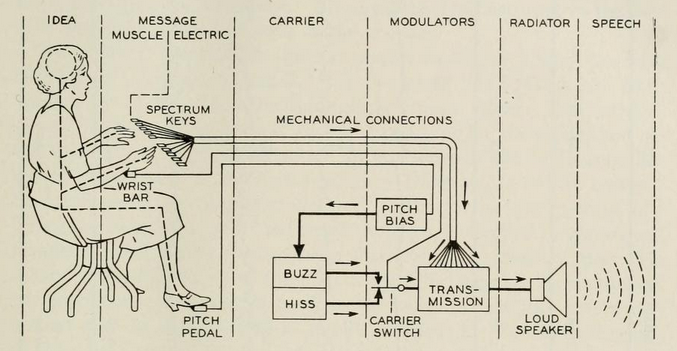
\includegraphics[width=\textwidth]{imagenes/Voder.png}
	\caption{Un esquema del \textit{Voder}. Extraído de \cite{voder}}
\end{figure}

La primera aplicación del reconocimiento de voz fue presentado por IBM en 1962. Con el nombre de \textit{Shoebox} \cite{shoebox}, era una calculadora capaz de reconocer 16 comandos (los dígitos, \textsc{Plus}, \textsc{Minus}, \textsc{Subtotal}, \textsc{Total}, \textsc{False} y \textsc{Off}). Su salida se emitía sin embargo en una impresora.

En 1961, el Doctor J.L Kelly usó un IBM 704 para sintetizar voz a través de un ordenador, cantando una canción en compañía de una orquesta. A partir de ese punto se ha ido trabajando en alas de una voz más natural que se pudiera lanzar con altavoces más pequeños.

En 1972, en el DARPA, se culminó un sistema más complejo de Reconocimiento de Voz denominado \textit{Harpy} \cite{harpy}, el cual permitía reconocer 1000 palabras e incluso sus combinaciones con tal de crear oraciones y sentencias.

En los 90, se empezó a vender programas software como \textit{Dragon Dictate} \cite{dragon-dictate}, que permitía reconocer bastantes palabras y que se distribuía de forma comercial al público, aunque el monto a gastar por entonces era de 6000 dólares.

\subsubsection{Los primeros Asistentes Virtuales: el don artificial del habla}

El campo de los Asistentes Virtuales ha sido basado en texto durante bastante tiempo, donde a través de un globo podías leer sugerencias y consejos (como ejemplo podemos poner a Clippy, incorporado en 	Microsoft Office 97). Pero hubo dos grandes eventos que dieron pie a la actualidad de los Asistentes de Voz, solapando la los años más recientes. En general, la década de los 2010 ha sido la que estamos continuando actualmente.

\begin{itemize}
	\item Por una parte, el equipo \textit{DeepQA} de IBM \cite{deepqa} se dedicó desde 2004 a hacer un sistema que pudiera responder cualquier pregunta hablada. Este fue más conocido por ganar en simulacros de \textit{Jeopardy} contra campeones de ese programa en 2010 y 2011.
	\item Por la otra, la popularización de los \textit{smartphones} con los iPhone de Apple y la compra de Siri para su posterior mejora, dio la popularidad de los Asistentes Virtuales de Voz que conocemos actualmente.
\end{itemize}

\subsection{En la actualidad...}
Esta era es el apogeo de los Asistentes Virtuales, que están empezando a desarrollarse en multitud de formatos por parte de varias compañías conocidas. En esta parte hablaremos de algunos de ellos a modo introductorio, aunque en el Análisis hablaremos en detalle y analizaremos competitivamente sus habilidades.

\subsubsection {Aplicaciones populares}
Hoy en día, las empresas más importantes tienen una instancia de Asistente Virtual por voz. Comentemos algunas de ellas:

\begin{itemize}
	\item \textbf{Apple Siri} \cite{siri} Como se comentó previamente, fue el resultado de la compra de esa aplicación, la cual se integró en el iPhone 4S para darle distintivo a sus dispositivos, presentándose el 14 de Abril de 2011. Con el tiempo se fue extendiendo a los aparatos de Apple, formando parte de su ecosistema.
	\item \textbf{Google Now} Al principio fue diseñado como un sistema de tarjetas que iba aprendiendo de las búsquedas e información del usuario para dar información relevante, pero este no respondía con voz. Posteriormente evolucionó a \textbf{Google Assistant} \cite{google-assistant} en Mayo de 2016, primero como parte de una app y extendiéndose de forma análoga a Siri en los dispositivos del ecosistema de Google y Android, siendo este software el que lo enmarca en esta lista.
	\item \textbf{Amazon Alexa} \cite{alexa} Alexa fue presentada en Noviembre de 2014 para dispositivos Echo. Debido a la gran infraestructura que posee esta multinacional en cuanto a servidores y servicios de \textit{cloud} se refiere, gran parte de ese procesamiento pasa por esas infraestructuras. Además permite hacer aplicaciones (o \textbf{skills}) para que terceros puedan integrarse con este Asistente. Actualmente ha sido integrado en multitud de dispositivos incluso fuera de su ecosistema.También se está ofreciendo como un \textit{SaaS} (\textit{Software as a Service}) para poder integrarlo donde se pueda, además de ciertos plus como voces de famosos.
	\item \textbf{Microsoft Cortana} La respuesta por parte de la empresa de Bill Gates ante el boom del tema a discutir, y tomando la inspiración de una de los personajes más icónicos de \textit{Halo} (uno de los juegos más famosos de la consola de la compañía, \textit{Xbox}), fue presentada en una conferencia de la empresa en Septiembre de 2014. Con la llegada de Windows 10, este asistente llegó integrado. Hay constancia de dos versiones para Android y iOS, pero sólo en inglés. A día de hoy, se están redirigiendo los esfuerzos del proyecto de cara a la productividad empresiaral con la línea de Microsoft 365 \cite{cortana}.
\end{itemize}

Además de estos, hay un montón más de ellos. En algunos casos, se crean por la falta de soporte de alguno de las empresas más grandes (por ejemplo, \textbf{Huawei Celia} \cite{huawei-celia} fue desarrollado por las restricciones de Estados Unidos). En otros, por tener otras alternativas con filosofías como el \textit{FOSS}, del cual hablaremos posteriormente. Un ejemplo de ello es \textbf{MyCroft} \cite{mycroft}, que asegura la privacidad de la información y la apertura de su código, además de ofrecerse como una alternativa ligera en cuanto a recursos.

Posteriormente haremos un análisis competitivo de estas opciones a fin de comparar su funcionamiento y prestaciones, para hacernos una idea general de posibles mejoras.


\subsubsection{Un sinfín de formatos}
Hoy en día, podemos encontrarnos estas aplicaciones casi en cualquier lado. Si bien en un principio estaba pensado para smartphones, enseguida fue adaptado a otros aparatos.
Una de las propuestas fue con Amazon y su asistente Alexa, que fue embebida en un dispositivo sin pantalla llamado Echo \cite{echo}. Sólo dispone de altavoces, micrófonos, una luz para saber si escucha y se podía conectar con el teléfono para poder insertar las contraseñas pertinentes. Posteriormente se hizo una versión que tenía una pantalla para mostrar algunas cosas.
Gracias a la variedad de versiones de ese producto, se permite tener uno de esos Asistentes por precios más o menos caros, con calidades más o menos Premium.

En general, los movimientos en estas aplicaciones tienden a comenzar en un pequeño sector el cual trata de expandirse para formar parte de la experiencia de un ecosistema donde se ha desarrollado.

\begin{figure}[p]
	\centering
	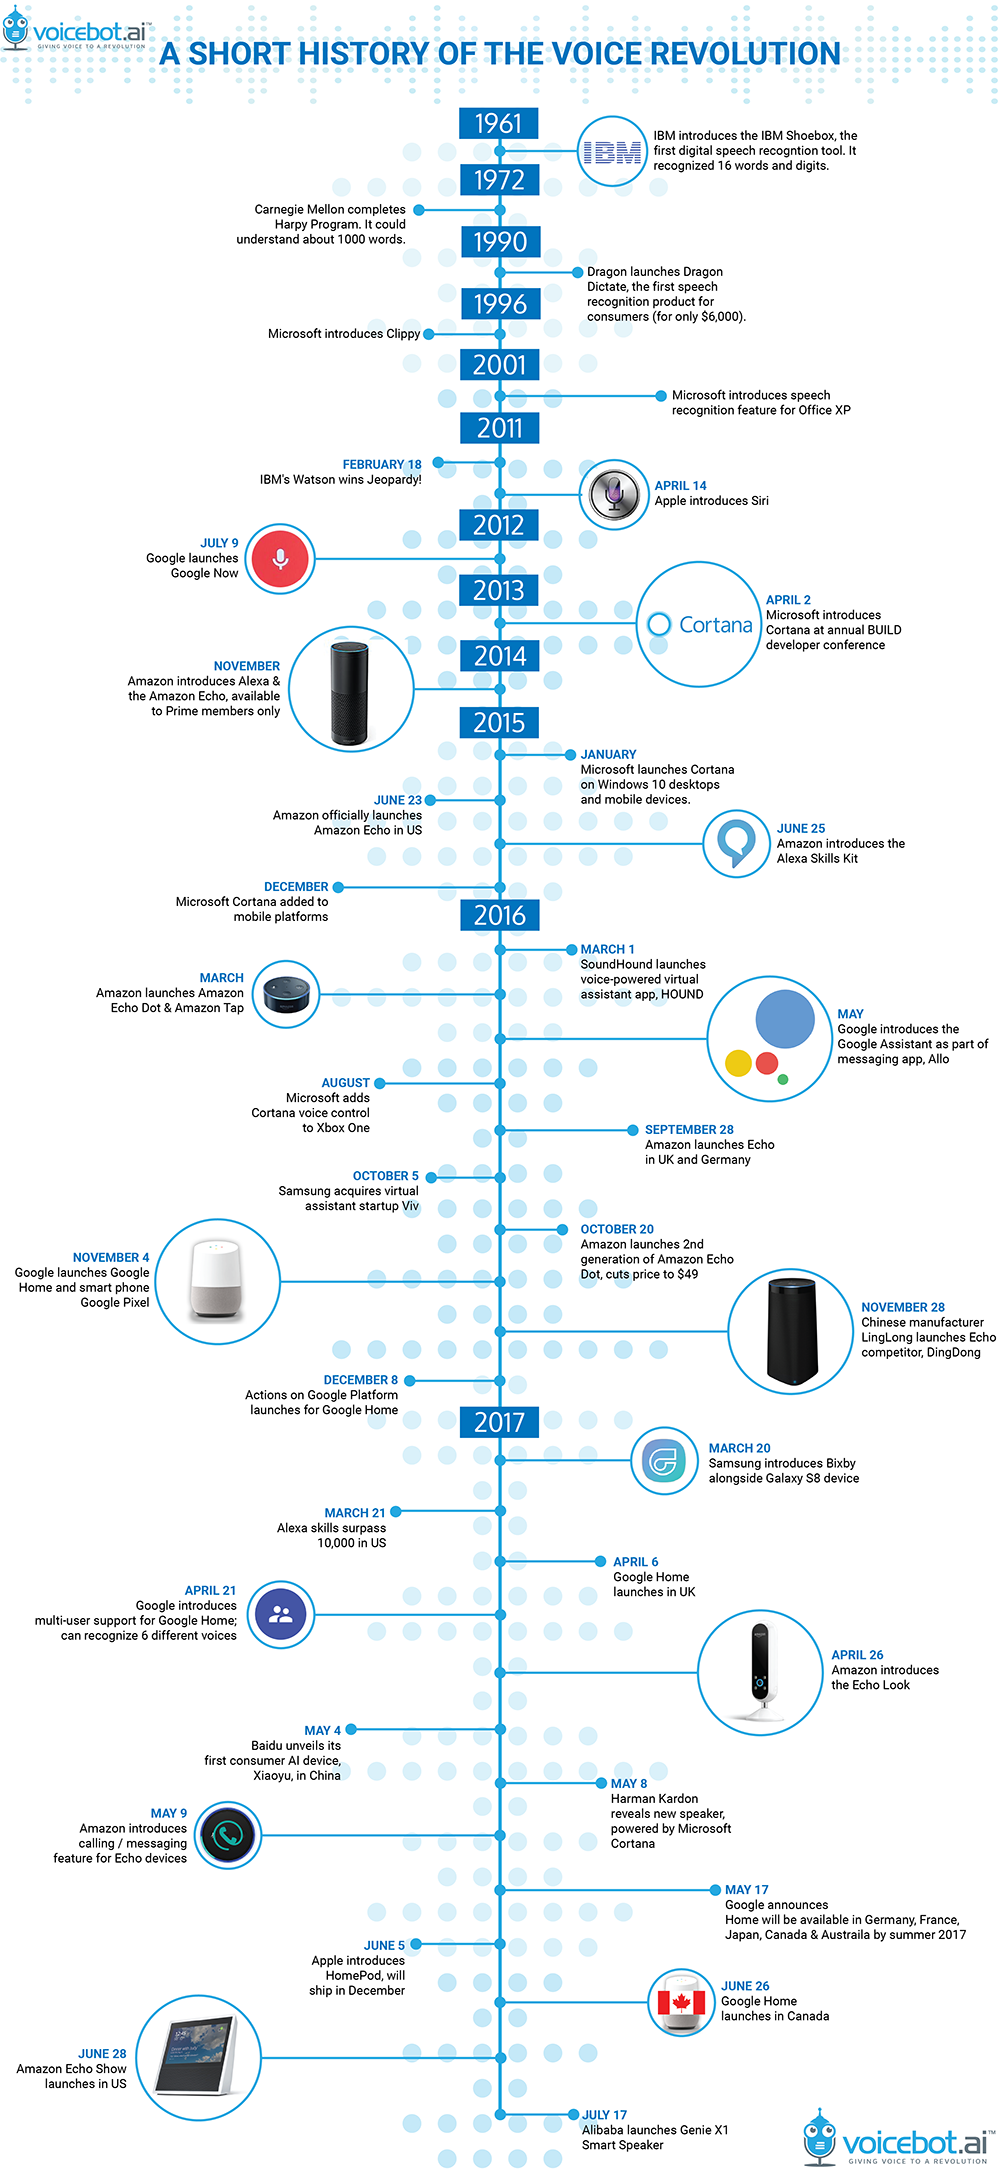
\includegraphics[height=0.98\textheight]{imagenes/Timeline_VA.png}
	\caption{Una timeline con algunos de los eventos más importantes en el área. Extraído de \cite{va-history}}
\end{figure}

\subsubsection{Las ventajas}
 \begin{itemize}
 	\item Una de las más notorias, como hemos visto, es que podemos tener uno de ellos en cualquier sitio. Como hemos comentado antes, desde dispositivos dedicados como los altavoces inteligentes, pasando por ordenadores y \textit{smartphones}, hasta aparatos del Internet de las cosas como \textit{Smart TVs}.
 	\item La información se está solicitando y recibiendo usando la voz, por lo que no es necesario usar las manos o la vista (como hemos comentado en la Introducción), por lo que uno de los usos sería para personas ciegas o con diversidad motora (véase, por ejemplo, la cuadriplejía). Pero además es un punto de acceso para aquella gente que tampoco sepa o pueda leer o escribir, gracias a cómo se puede comunicar la información.
 \end{itemize}
\subsubsection{Las desventajas}
	\begin{itemize}
		\item La más importante está relacionado con la seguridad y privacidad de lo que se usa en ello. Matthew Hoy \cite{vaintroduction-matthewhoy} comentaba en su Introducción a los Asistentes Virtuales que se podría preguntar al propio asistente por información de aquellas cuentas e integraciones que tenga conectadas, o pedirle que le haga tareas.
		
		Como adición a ese comentario, decir algunas de ellas no reconocen exactamente de quién es la voz, por lo que sintetizar la voz para un comando o tener el altavoz de algún dispositivo cerca de este e invocar al software durante una llamada podría ser suficiente para que el Asistente funcione y ejecute lo que se quiera.
		
		Como extra, tengamos en cuenta que uno de los componentes principales de un Asistente de Voz es un micrófono. Aunque conceptualmente sólo sirva para cuando se le llama explícitamente, este igualmente está grabando mientras espera a que se diga su palabra de invocación (o \textit{trigger word}). Como consecuencia, puede generar cierto alarmismo por ese hecho y, en el caso de que alguien pudiera lograr usar ese micrófono para obtener las grabaciones con otros propósitos, generar una brecha de privacidad que podría ser explotada.
		
		\item Si bien se han hecho progresos en los campos del \textit{Speech Recognition} y el \textit{Text-To-Speech}, no son perfectos. Por lo tanto, es posible que ante una petición el comportamiento puede ser un poco indeterminado según la tolerancia del Reconocedor, su entrenamiento y cómo el usuario se exprese.
		
		Por otra parte, la voz que se sintetiza puede llegar a resultar algo robótica, aunque se tratan de hacer esfuerzos en que se intente ser más natural. La otra opción, si se quisiera ser totalmente natural, sería que alguien grabara las voces y estas se reproduzcan, pero además de resultar algo tedioso ya que pueden haber muchas respuestas por grabar, ocupan mucho espacio, algo no muy deseable.
	\end{itemize}

\section{Fundamentos de los Asistentes de Voz}
Por lo analizado a través de la historia y la situación actual podemos intentar extraer un marco teórico que recogería todos los elementos de los Asistentes de Voz y cómo se combinarían para formar algo.

\subsection{Una idea intuitiva}
Para empezar, podríamos empezar con lo que haría un \textit{software} convencional. Se alimenta con una serie de datos, se procesa y acaba saliendo otra serie de datos. Si representáramos ese concepto en un diagrama, tendríamos lo siguiente:

\begin{figure}[H]
	\centering
	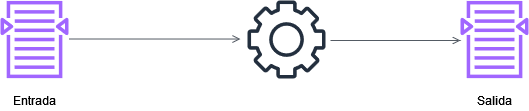
\includegraphics[width=\textwidth]{imagenes/DiagramaBase.png}
	\caption{Diagrama básico de un software. De elaboración propia.}
\end{figure}

Los datos que recoge, en nuestro caso, son voces. Por el otro extremo, lo mismo. Podríamos actualizar nuestro diagrama con esa salida.

\begin{figure}[H]
	\centering
	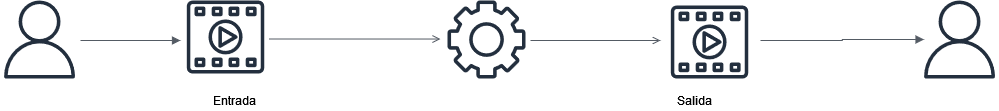
\includegraphics[width=1.1\textwidth]{imagenes/DiagramaDatos.png}
	\caption[Diagrama modificado.]{Diagrama modificado. Nótese que en vez de documentos se usa multimedia. De elaboración propia.}
\end{figure}

Esas voces que se recogen no se generan solas. En el caso de la recogida, es un usuario quien habla a través de un micrófono para grabar esa voz que podrá procesar posteriormente. En el otro lado, esa voz se reproducirá a un altavoz. Esos procesos de grabación y reproducción tienen ya de por si su propia lógica intermedia para poder procesarlos. Con esta nueva información, el diagrama quedaría de la siguiente forma:

\begin{figure}[H]
	\centering
	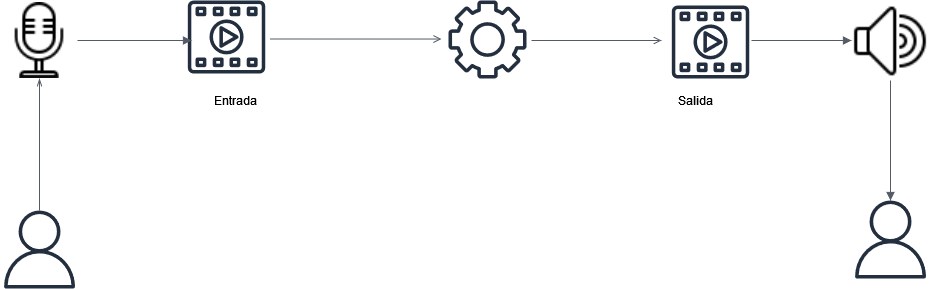
\includegraphics[width=1.1\textwidth]{imagenes/DiagramaIO.png}
	\caption[Diagrama con E/S.]{El mismo diagrama que el anterior, pero señalando las Entradas y Salidas. De elaboración propia.}
\end{figure}

Ahora tenemos otras dos cuestiones sobre esos archivos de audio.
\begin{itemize}
	\item ¿Cómo puede entender \textbf{qué está diciendo esa voz}?
	\item ¿Cómo se crea \textbf{el audio de la respuesta} a partir de un texto?
\end{itemize}
La respuesta a esas dos preguntas resulta ir en dos campos respectivos de la Inteligencia Artificial: el \textbf{Reconocimiento} (o \textit{\textbf{Speech Recognition}}) y la \textbf{Síntesis de Voz} (conocido más como \textbf{\textit{Text-to-Speech}}). 

Por lo tanto, se crea una lógica para poder hacer esas conversiones, de forma que podríamos hacer que el sistema nos escriba qué ha entendido (reconociendo esa voz) y que ``lea'' la respuesta con lo que le hayamos escrito (sintetizando la voz). De todas maneras, hablaremos de ello más adelante. Podríamos actualizar el diagrama resultando en esta figura.

\begin{figure}[H]
	\centering
	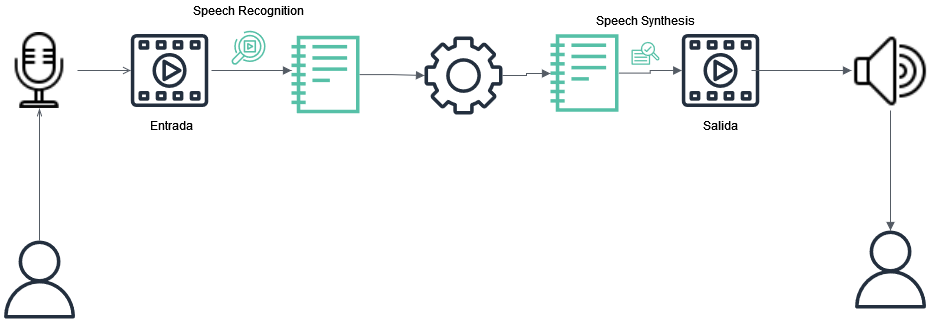
\includegraphics[width=1.1\textwidth]{imagenes/DiagramaTTS_SR.png}
	\caption[Diagrama con TTS/SR]{El diagrama anterior pero señalando las interacciones con el Speech Recognition y el Text-To-Speech (o Speech Synthesis). De elaboración propia.}
\end{figure}

Por último, la lógica que hay entre lo que se ha dicho y lo que tiene que leer la máquina debería poder procesar esa frase, buscar si sigue algún patrón o usa alguna palabra de relevancia (como ``Reproduce'', ``Canta'' o ``El tiempo en una ciudad''), y dar una respuesta que se pueda leer. Por lo tanto, el diagrama final a modo conceptual podría darse como la de la siguiente figura: 

\begin{figure}[H]
	\centering
	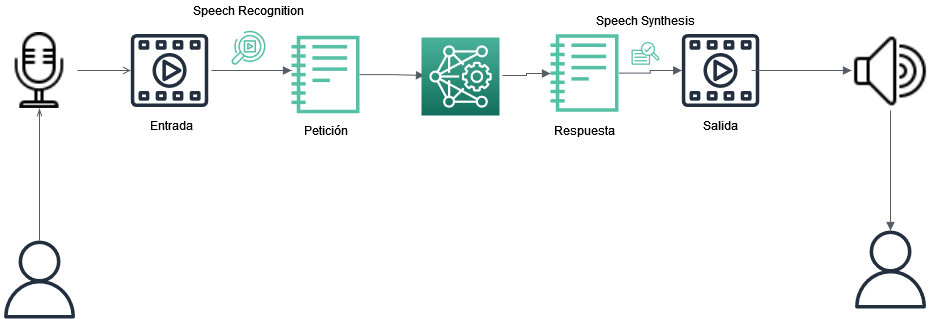
\includegraphics[width=1.1\textwidth]{imagenes/DiagramaIntuitivo.png}
	\caption[Diagrama intuitivo final.]{Diagrama resultante. Nótese que la lógica en verdad es un proceso de relacionar conceptos. De elaboración propia.}
\end{figure}

En resumen, podríamos decir que un Asistente de Voz consta a nivel \textit{hardware} de un ordenador con un micrófono o entrada de audio y un altavoz o salida de audio.

Sin embargo, a nivel \textit{software} necesitaríamos:
\begin{enumerate}
	\item Un módulo para gestionar las \textbf{grabaciones del micrófono} que diga cuándo grabar, cuando parar, y que guarde la grabación para poder trabajar con esta. Esta nos devuelve un audio
	\item Una parte para hacer \textbf{Reconocimiento de Voz} a través de esa grabación. Nos devuelve el mensaje de ese audio.
	\item La \textbf{lógica principal} del programa, que mira el mensaje y responde con otro.
	\item Una parte para poder hacer \textbf{Text-To-Speech}, convirtiendo la respuesta en otro audio.
	\item Un módulo para poder \textbf{reproducir ese audio} con la respuesta a través del altavoz, que cargue el archivo y lo reproduzca.
\end{enumerate}

\subsection{El reconocimiento de voz}
En la documentación sobre el tema, IBM \cite{sr-definition} define el Reconocimiento de Voz o \textit{Automatic Speech Recognition} (ASR) como la capacidad de un programa de procesar el habla y convertirlo en un texto escrito legible, que puedan entender también las máquinas para el posterior procesado de la información.

Para poder reconocer esa voz, se necesita primero separar ese sonido en pequeños fragmentos que pueda comparar con un Modelo Acústico (es decir, un conjunto de sonidos pequeños que se conoce lo que significa), de forma que se pueden asociar los del audio enviado con estos para buscar similitudes. Con ello, se busca en un Modelo del lenguaje (un conjunto de letras o combinaciones de estas asociadas a ese sonido) qué palabras quieren decir, y las compara para dar un porcentaje de acierto. Finalmente devuelve un texto o varias versiones de un texto según las opciones que haya ido observando.

Uno de los grandes retos en este campo viene porque no todos tenemos la misma voz, y por lo tanto si bien los Modelos Acústicos pueden reconocer muchas de ellas, no puede con todas, y es imposible tener todas las voces almacenadas. por lo tanto, se han pensado en varias maneras de abordar ese problema a través del Aprendizaje Automático. Mencionaremos algunas de ellas en estos epígrafes a un nivel introductorio. \cite{sr-methods}

\subsubsection{Modelos de mezcla Gaussiana} 
Una primera tarea para abordar este campo sería usar la probabilidad de que el sonido coincida con lo que tiene en su modelo, pudiendo así saber qué sonido tiene cada uno.

Si representáramos en una gráfica dos variables (como el fonema y el tiempo), podríamos ver que esos puntos se podrían agrupar en \textit{clusters} que se acercan a ese fonema para dar con la media de ellos y sacar el que más se parezca al resultado, haciendo así una clasificación de los sonidos. Eso es precisamente cómo funciona el modelo de mezcla gaussiana.

Un modelo de mezcla Gaussiana \cite{gaussiana} es un modelo probabilístico que asume que todos los puntos a analizar se han generado a través de varias distribuciones gaussianas juntas (una cantidad $K$ de ellas). Por lo tanto, un punto en el plano puede estar cerca de un punto intermedio de esos $K$ que representa una de las distribuciones que se han mezclado, dando a entender que ese punto sea más probable de pertenecer a esa distribución que a otra.

\subsubsection{Modelos ocultos de Markov} 

El propio hecho de intentar predecir qué va a decir alguien es un tanto arduo, ya que el mensaje que vas a comunicar puede ir completándose durante el tiempo que se está hablando. Podríamos decir entonces que el hecho de hablar es dar una cadena donde nos vamos enterando del mensaje por la secuencia de sonidos aleatorios, generando fonemas que se unen y comparan con los modelos para encontrar las palabras.

Al final, podríamos darnos con esta serie de condiciones:
\begin{itemize}
	\item Tenemos un tiempo que podemos cuantificar discretamente : $ t \in \{1,2,3...\} $
	\item Cada instante tenemos unas variables aleatorias que podemos o no observar (por ejemplo, la frecuencia del sonido o la letra que intenta decir)
	\item Las relaciones entre los estados de esas variables según el tiempo sólo dependen del estado anterior (en nuestro caso, si se intenta decir \textit{mesa}, se debería escuchar primero la letra \textit{m}, luego entender \textit{me}, y así sucesivamente)
	\item Los estados finales que puede tomar cada sonido al final se pueden relacionar con una letra o conjunto de ellas, que si bien es un conjunto grande, al menos es finito.
\end{itemize}

Esto podría ser por lo tanto un caso de aplicación de un \textbf{Modelo Oculto de Markov}\cite{modelo-markov}, donde tenemos por una parte una variable aleatoria de estado que no se puede observar directamente (cómo en nuestro caso la letra o fonema que va a decir) y por la otra una variable que sí podemos observar directamente (por ejemplo, si grabamos ese sonido y sacamos su representación de las frecuencias).

Este modelo posee dos propiedades que tienen cabida en el contexto que presentamos:
\begin{itemize}
	\item \textbf{Propiedad de Markov} En cada instante, el estado sólo depende del estado anterior. En nuestro caso, si en un instante $t$ se tiene la alta probabilidad de que un sonido se asocie con una consonante, en la siguiente ($t+1$) habría una gran probabilidad de que fuera una vocal, visto lo anterior.
	
	\item \textbf{Independencia de las percepciones} En cada instante, lo observado sólo depende de ese instante. Si en el caso del Reconocimiento de Voz tuviéramos en cuenta el sonido de antes, sería muy difícil saber qué fonemas suenan en cada momento para poder asociarlos correctamente, dando lugar a errores de comprensión.
\end{itemize}

Así, podríamos ver ese modelo como una especie de máquina de estados basado en una serie de probabilidades de que cambie de un estado a otro según lo que se observe.

\subsubsection{Redes neuronales en el ámbito del Speech Recognition}
Las redes neuronales son en esencia nodos con varias entradas que tienen asociados un peso o importancia a tener en cuenta, que se van ajustando según las conexiones en un grano más fino y se concentran en un resultado final que activa o desactiva.

De esta forma, primero se entrena la red neuronal con una serie de datos que se saben qué resultado tienen para poder ajustarlo; y una vez entrenado, ya se puede dejar con datos que no se han probado.

\subsubsection{Frameworks y librerías}

Hoy en día hay servicios a través de la nube que ofrecen APIs que permiten el reconocimiento de voz, además de softwares y librerías que permiten hacerlo de forma local, aunque al estar orientado a modelos embebidos tienen un reconocimiento más limitado que a través de servidores que pueden almacenar más sonidos y relaciones.

En cuanto a servicios en la nube podemos destacar \textbf{IBM Watson} \cite{ibm-sr}, \textbf{Amazon Transcribe} \cite{amazon-transcribe} o \textbf{Google Cloud} \cite{google-stt}, los cuales usan sus soluciones para ofrecer una API que permite obtener el audio a partir de una serie de instrucciones contenidas en una biblioteca o en varios endpoints.

Sobre las soluciones más limitadas pero locales, podemos hablar de \textit{Vosk API} \cite{vosk}, que tiene modelos de 50 MB para idiomas como el Español, el Inglés o el Catalán.


\subsection{La síntesis de voz}
Si el reconocimiento de voz trata el procesamiento del habla para extraer un texto, la síntesis de voz sería lo contrario, la producción artificial de ese habla \cite{tts-definition}. 

Para ello se usan como base los grafemas (aquellas letras y grupos que se pronuncian de una manera). De esa forma, se separa el texto en dichos grafemas, tras lo cual se asocian esos grafemas a sus correspondientes sonidos o fonemas asociados, entonando así cada palabra, frase y finalmente leyendo el texto.

Eso sí, de forma similar al Reconocimiento de Voz, tienen un Modelo para asignar los fonemas a sus grafemas. Aunque en este caso se simplifica el modelo acústico ya que se usa una serie de sonidos predeterminados para darle una voz al resultado.

Uno de los grandes retos que se ha ido viendo mejoría es la naturalización de la voz que sintetiza. Si bien ha habido una mejora desde su creación y aún va evolucionando año tras año, todavía queda camino para llegar a una voz que no pudiéramos etiquetar como robótica.

Al ser el Reconocimiento y la Síntesis de Voz procesos contrarios, se pueden emplear los mismos métodos para hacer una u otra cosa.

En cuanto a soluciones ya implementadas, por parte de la nube tanto Amazon \cite{polly} como IBM \cite{ibm-tts} y Google \cite{google-tts} también tienen su TTS, y si hablamos de software local tenemos opciones como Festival \cite{festival} o las voces preinstaladas en Microsoft, o Siri en caso de los Mac.
 

\subsection{La lógica}

La lógica del proyecto se puede parecer al de un chatbot de texto, el cual tiene como unidad básica las palabras, que se unen para poder encontrar sentencias o patrones que puede usar para asociarlas con una respuesta y así enviarlo al usuario.

La primera aproximación para tener ese bot funcionando sería ir comprobando que lo que se envíe tenga una palabra clave que pueda buscar para saber si debe actuar \cite{chatbots-architecture}. Pero las respuestas serían bastante estáticas.

Una evolución de ello es que reconozca varias palabras en conjunto, o que admita múltiples palabras para llegar al mismo resultado, dando así un poco más de responsividad ante varias maneras de hacer la misma petición, pero no arreglaría lo primero.

Podríamos entonces añadirle algunas peticiones que requieran de algo variable, como preguntar por el tiempo en una ciudad. De esta manera, las respuestas son más personalizadas para cada uno. El problema con esta iteración es que hay que saber dónde buscar esa información, pero hoy en día está solventado ya que gracias a la aparición de APIs y conexiones con Bases de Datos se pueden enriquecer esas mismas respuestas.

Estas ideas han dado lugar a algunos lenguajes de marcado basados en \textit{pattern matching} que permiten realizar esas distinciones para dar respuestas. Podemos listar algunas de ellas:
\begin{itemize}
	\item \textbf{AIML (\textit{Artificial Intelligence Markup Language})} \cite{aiml} Es un lenguaje basado en XML que permite realizar algunas cosas básicas como guardar información básica, usar datos descritos en el patrón para devolverlos y decir respuestas aleatorias. Fue pensado para usarse en otro programa llamado \textit{AliceBot}, pero hay programas que permiten realizar el \textit{parsing} de documentos de este tipo.
	
	La base de AIML son las categorías, que dentro tienen patrones que escriben los usuarios y plantillas que devuelven los bots.
	
	\item \textbf{RiveScript} \cite{rivescript} Basado en AIML, pero en vez de usar los bloques de XML utiliza unos pocos símbolos.
	
	\item \textbf{ChatScript} \cite{chatscript} Basado en el Procesamiento del Lenguaje Natural, este lenguaje de scripting utiliza una serie de reglas para ejecutar las respuestas. Además permite hacer llamadas HTTP a servidores.
\end{itemize}

Aparte de esta aproximación, podríamos usar un algoritmo para buscar a partir de una serie de datos sobre qué se habla, o usar una serie de redes neuronales como el \textbf{NLP} (\textit{\textbf{Neural Language Processing}}) con tal de que esos patrones se estudien para dar después con unos nuevos, usando para ello \textit{Machine Learning} \cite{chatbots-architecture}

\section{Software Libre, Software de Código Abierto y Licencias}
El software libre y sus licencias \cite{gplv3} ha permitido llevar a cabo una expansión del aprendizaje de la informática sin precedentes. 

Como se ha comentado en el primer capítulo, sirve como respuesta a la colisión de la protección de las propiedades intelectuales de las empresas contra los derechos de los usuarios por los cuales, con una copia adquirida, no puedan emplear algunas herramientas para poder preservar el producto que ha adquirido de ellos. Además permite, igual que en la ciencia, compartir el conocimiento para construir a partir de ahí todo lo necesario.

Se ha llegado a un punto en la actualidad donde muchas de las herramientas más populares tienen una alternativa de software libre o ,al menos, de código abierto.

\subsection{¿Desde cuándo existe?}
La historia del software libre empieza más allá de que se acuñara ese término \cite{foss-history}. En los años 60, era muy común que aquellos con la suerte de tener un ordenador trataran de facilitar el código de sus programas entre ellos. De hecho,las compañías que manufacturaban esos ordenadores no hacían la separación comercial del software dentro de las capacidades del computador.

Ya en la década de 1970, empezaron a surgir empresas que comerciaban software de forma explícita, de forma que fuera compatible con hardware diseñado por otros con el objetivo de lucrarse con estos programas. Para limitar lo que podían hacer con esas aplicaciones, estas compañías ponían trabas a la hora de compartir, modificar y estudiar su producto.

Como respuesta a ellos, y sobre todo en los centros universitarios como \textit{Berkeley} o \textit{Massachussets}, se formaron grupos académicos que distribuían sus programas de forma libre, siendo éstos un esbozo de lo que se conocen actualmente como grupos \textit{FOSS} (de \textit{Free and Open Source Software}) 

Los hitos más relevantes en esta línea temporal fueron el desarrollo del Proyecto GNU de Richard Stallman, quien  sentó las bases de la iniciativa del Software Libre con sus 4 libertades \cite{fsf-philosophy} que permiten el uso, modificación, compartición y estudio de aquel software que estuviera forjado con esa filosofía. Empezando como un proyecto que perseguía hacer un Sistema Operativo similar a Unix, sirvió para realizar montones de utilidades que seguimos usando aún a día de hoy, gracias a la aparición del segundo hito relevante.

Este segundo hito no es ni más ni menos que la creación de Linux por el finlandés Linus Torvalds, que si bien al principio no estaba puesto como Software Libre, en su versión 0.12 \cite{linux-releasenotes0.12} se cambió a tal, lo que fue del agrado del proyecto GNU. Junto con la propagación del nuevo SO y la adaptación de las herramientas de GNU a este, se consolida una base sobre la que empresas y fundaciones dedicadas al \textit{FOSS} realizan compilaciones y variaciones sobre el núcleo dando lo que se conocen como \textit{distros}.

\subsection{¿En qué beneficia liberar el código?}
En una charla sobre Software Libre se discutió este punto \cite{osl-charla-liberatucodigo}, llegando a 4 grandes beneficios que enumeraré a continuación:

\begin{enumerate}
	\item \textbf{Esforzarse en cumplir con buenas prácticas de desarrollo} Al ser un código que todo el mundo va a ver, puede servir para acostumbrarnos a tomar buenas prácticas de desarrollo, como el Test Driven Development, seguir patrones y arquitecturas de diseño software
	\item \textbf{Generar una comunidad y/o participar en otras} Al liberar el código, por una parte colaboras en el mundo del software libre ofreciendo un nuevo proyecto que pueden estudiar y usar como alternativa a otros; y por otra generar una comunidad alrededor del proyecto a través de aportes, discusiones, documentación...
	\item \textbf{Añadir un proyecto al portfolio personal} Siendo esta la parte más individualista de las ventajas, tener un proyecto en una forja como \textit{GitHub} permite a las empresas ver cómo trabajas y qué cosas te interesan de cara al mundo laboral y empresarial.
	\item \textbf{Generar un ejemplo a la comunidad de desarrolladores} Al liberar el código das una condición de transparencia a todo lo que se hace, cosa que viene bien en instituciones públicas como Universidades o Empresas asociadas al Estado.
\end{enumerate}



\subsection{El curioso mundillo de las Licencias y sus restricciones}

Uno de los puntos más interesantes del Software Libre es que para poder proteger y asegurar que las condiciones de ésta se cumplan, hayan recurrido a crear un entorno legal que sirva de punto de referencia sobre la que partir y ayudar al desarrollo de proyectos dentro de este marco. \cite{foss-marcojuridico}

\subsubsection{Detallando el marco legal de las Licencias}
Las licencias son, como bien hemos dicho previamente, un contrato entre la persona que lo crea y el desarrollador que quiere aplicarlo en su proyecto. Esto da lugar a una serie de condiciones que deben cumplir ambas partes con tal de llegar a un punto donde ambas partes estén de acuerdo. En general se aplican licencias genéricas hechas por organismos reconocidos como la \textit{Free Software Foundation} o \textit{Creative Commons}, pero si se sabe de legislaciones y cumplen con la finalidad de poder estudiar y usar sin muchas restricciones, se podría realizar y usar.

Vamos a hablar de algunas de las licencias más comunes usadas en el ámbito del Software Libre e incidiremos en el punto de la creación de licencias.

\subsubsection{Free Software Foundation}
Creadas en 1989, se crearon las licencias GPL con el objetivo de proteger el software del proyecto GNU de que terceros hicieran algunas modificaciones que explotaran en un software privativo.

Si bien al principio fue una licencia popular, este llevaba a que encontraran una serie de brechas en la descripción de la licencia. Estas eran \cite{gplv3-changelog}:
\begin{itemize}
	\item \textbf{Tivoización} En honor a los aparatos de recepción de vídeo TiVo, es el hecho de que el software con posibilidad de modificación no se pudiera instalar en esos receptores ya que el hardware no lo soportaría.
	
	\item \textbf{Compatibilidad con el Affero GPL} debido a que no había cláusulas sobre el software en red.
	
	\item \textbf{Cláusula contra las represalias de patentes} Si bien en España y la mayoría de países se protege el software a través de los derechos de autor, en países como EEUU o Japón se puede patentar, y con esta versión se persigue que haya un amparo legal contra quienes intenten patentar el software libre y usen esas herramientas legales a quienes deseen modificarlo. De esta manera se hace un control de daños, ya que no se puede como tal evitar patentar versiones modificadas de un software libre.
	
	\item \textbf{Protección para herramientas contra el DRM} de forma que se pueden publicar programas que jueguen con la protección de los derechos de autor sin romper leyes de ese tipo, como el DMCA estadounidense.
	
\end{itemize} 

Todo ello se resolvió con la versión 3 de sus licencias. \cite{gplv3-changelog}

Por parte de la FSF, se han creado 3 licencias que se usan popularmente en este mundillo:

\label{gpl-license-types}
\begin{itemize}
	\item \textbf{GPL : \textit{GNU Public License}} Esta licencia trata de declarar que el software es libre y protegerlo a su vez de apropiaciones indebidas, de forma que quien quiera pueda estudiar, usar, compartir y modificar. 
	\item \textbf{LGPL: \textit{Lesser GNU Public License}} Es similar a la anterior, pero se diferencia en que el software puede formar parte de software privativo.
	\item \textbf{AGPL: \textit{Affero GNU Public License}} Esta licencia hereda de GPL casi todo su contenido, al que además se le añade una nueva cláusula que obliga a distribuir ese software si se ejecuta dando servicios a través de una red de ordenadores.
\end{itemize}

\subsubsection{Creative Commons}
Creative Commons \cite{cc-about} es una organización que se dedica a proveer de herramientas legales para poder compartir el conocimiento y la cultura (no exclusivamente al código). Esas herramientas son en realidad una serie de licencias modulares que permiten restringir o ceder en una serie de aspectos:

\begin{itemize}
	\item \textbf{BY (Reconocimiento) - } Pide que si se usa en algún lugar, se mencione al autor de éste
	\item \textbf{NC (No comercial) - } Prohíbe que se use la obra con fines comerciales
	\item \textbf{ND (Sin derivaciones) - } La obra puede permitir obras derivadas a partir del original.
	\item \textbf{SA (Share-Alike o Compartir-Igual) - } Pide que quien vaya a usar la obra lo comparta en las mismas condiciones que el original.
\end{itemize}

Si bien en su versión 4.0 no se puede aplicar ya a software (aunque sí podría usarse, por ejemplo, para su documentación), en versiones anteriores mantiene su estructura \cite{cc-licenses}, siendo esta basada en una escala de más a menos restricciones, quedando en el siguiente orden:

\begin{itemize}
	\item \textbf{CC BY-NC-ND (Reconocimiento + No Comercial + Sin Derivaciones)}
	\item \textbf{CC BY-NC-SA (Reconocimiento + No Comercial + Compartir Igual)}
	\item \textbf{CC BY-NC (Reconocimiento + No Comercial)}
	\item \textbf{CC BY-ND (Reconocimiento + Sin Derivaciones)}
	\item \textbf{CC BY-SA (Reconocimiento + Compartir Igual)}
	\item \textbf{CC BY (Reconocimiento)}
	\item \textbf{CC 0 (Zero)} La obra es totalmente libre de usarse, el autor cede todos los derechos al usuario. Se conoce como \textit{Dominio Público}.
\end{itemize}

\subsubsection{Otros tipos de licencias}
Otras empresas, organizaciones e individuos han creado otras licencias cambiando algunos aspectos pero continuando con el esfuerzo de GPL de crear un contrato que defina los límites de la distribución y ampara al desarrollador. A modo de reseña, listo algunos de ellos.

\begin{itemize}
	\item \textbf{Licencia MIT} \cite{mit} Esta licencia es de tipo permisivo, por el cual sólo pide preservar los avisos de derechos de autor, aunque el usuario puede controlar más aspectos como, por ejemplo, vender el software final con las variaciones, o directamente cambiar la licencia. 
	\item \textbf{Licencia Apache} \cite{apache-license} Similar a la del MIT, permite no entregar el código fuente si se ha modificado sobre el proyecto original.
	\item \textbf{The Unlicense} \cite{unlicense} Similar a Creative Commons Zero, cede al dominio público el software resultante.
	\item \textbf{Licencias cómicas} A modo de sátira, se crearon algunas licencias por parte de algunos desarrolladores que a efectos legales tienen validez, pero no son muy aplicables en la práctica.
	 Entre ellos están el \textit{Beerware} \cite{beerware} (Sólo añade que si te encuentras con quien creó el software, le invites si quieres a tomar algo) o el \textit{Chicken Dance} \cite{chicken-dance}, que comenta que por cada 1000 copias vendidas de este software, al menos la mitad de la compañía tiene que bailar una canción.
\end{itemize}

\subsubsection{¿Puedo crear una licencia?}
Como se ha adelantado en el principio, podríamos dar como respuesta corta un Sí. Sería tan simple como poner las cláusulas y aplicarla en un proyecto. 

Sin embargo, esto lleva también un trasfondo jurídico por el cual podría requerir la asistencia de un abogado o un asesor legal que tenga un mayor conocimiento en estos temas.
	
	\newpage 
	\chapter{Especificación de requisitos}

\noindent\fbox{
	\parbox{\textwidth}{
		En esta capítulo se tratarán de recoger todos los detalles que definan y limiten el funcionamiento de la aplicación.
	}
}

\section{Personas: ¿Quienes lo podrían usar?}

Para poder hacernos una idea de los posibles usos del Asistente de Voz se ha decidido crear una serie de personas ficticias que, para poder facilitar algún aspecto de su vida, puedan usar este producto.

El hecho de introducir personas para obtener requisitos viene a partir de que es un producto que desconocemos quién lo va a usar. No es un producto a medida mandado por alguien a quien podamos preguntarle por su visión de la aplicación final. Por ello, entra en juego este recurso. El uso de personas ficticias en desarrollo de software es una técnica que permite buscar cualquier problema que se pueda presentar si el concepto se llevara a producir, con tal de buscar soluciones o compromisos a asumir.

En las tablas de las siguientes páginas, podemos encontrar una información somera de estas personas:

\begin{itemize}
	\item \textbf{Irene Fernández}, una estudiante de Bachiller en una fase de exámenes finales antes de la Selectividad, donde acaba por planear su estudio y el tiempo que le queda para poder acabar el curso y entrar a su carrera vocacional en la Universidad.
	
	\item \textbf{Javier Pedrosa}, un funcionario que recientemente perdió parte de la visión por un accidente, entrando en una nueva fase de su vida donde la tecnología le ayuda a poder tener cierta autonomía.
\end{itemize}

Si bien estos casos pueden necesitar soluciones concretas, el objetivo con este proyecto es que si alguna función no se pudiera realizar en este momento, gracias a la modularidad cualquiera pudiera integrar alguna utilidad para suplir esas demandas.

\begin{table}[H]
	\centering
	\begin{tabular}{|l|l|l|} 
		\hline
		Nombre       & Irene Fernández & \multirow{4}{*}{
			\begin{minipage}[t]{0.4\textwidth}
				\begin{center}
					 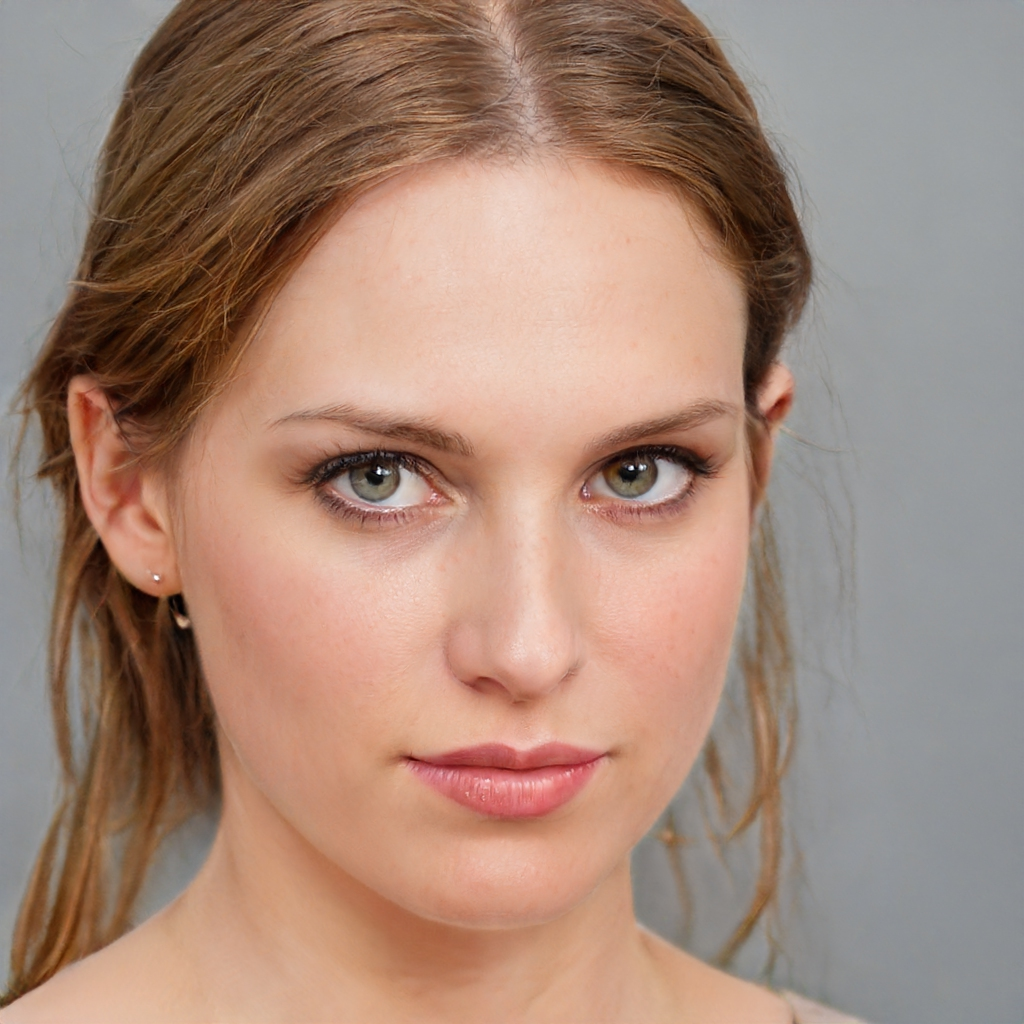
\includegraphics[height=3cm]{imagenes/Persona1.jpg}
				\end{center}
			\end{minipage}
			}                 \\ [2ex]
		\cline{1-2}
		Edad         & 19 &                                   \\ [2ex] 
		\cline{1-2}
		Género         & Femenino &                                   \\ [2ex]
		\cline{1-2}
		Educación    & Bachillerato Científico-Sanitario &                                   \\ [2ex] 
		\hline
		\multicolumn{3}{|l|}{{\cellcolor{lightblue}}\textbf{Contexto de uso}}               \\ 
		\hline
		Cuándo       & \multicolumn{2}{l|}{Tras las clases, antes de ponerse a estudiar}                \\ 
		\hline
		Dónde        & \multicolumn{2}{l|}{Ordenador portátil}                \\ 
		\hline
		\multicolumn{3}{|l|}{{\cellcolor{lightblue}}\textbf{Misión}}                        \\ 
		\hline
		Objetivo     & \multicolumn{2}{l|}{Tener una ayuda en el estudio}                \\ 
		\hline
		Expectativas & \multicolumn{2}{l|}{
			\begin{minipage} [t] {0.7\textwidth}
				\begin{itemize}
					\item Permitir hacer control del tiempo a través de contadores regresivos
					\item Permitir realizar cálculos sencillos
					\item Recordar tareas pendientes
				\end{itemize}
			\end{minipage}
		}                \\ 
		\hline
		\multicolumn{3}{|l|}{{\cellcolor{lightblue}}\textbf{Motivación}}                   \\ 
		\hline
		Urgencia     & \multicolumn{2}{l|}{
			\begin{minipage}[t]{0.7\textwidth}
				No le sería de mucha urgencia, ya que puede usar otras herramientas (Reloj/Cronómetro, Agenda, Calculadora...)
			\end{minipage}
		}                \\ 
		\hline
		Deseo        & \multicolumn{2}{l|}{
			\begin{minipage}[t]{0.7\textwidth}
				Siente que llevar tantas cosas para poder organizar su vida puede ser un tanto engorro, y centralizar sus utilidades en algo que lleve consigo como su portátil o su teléfono podría ahorrarle tantas molestias.
			\end{minipage}
		}                \\ 
		\hline
		\multicolumn{3}{|l|}{{\cellcolor{lightblue}}\textbf{Actitud ante la tecnología}}    \\ 
		\hline
		\multicolumn{3}{|l|}{
			\begin{minipage}[t]{\textwidth}
				Sabe manejar el ordenador en programas de ofimática como Word y Powerpoint; usa el navegador constantemente para ver sus redes sociales y buscar lo que necesite
			\end{minipage}
		}                              \\
		\hline
	\end{tabular}
	\caption[Ficha Persona 1]{Ficha de la Persona 1 (Irene Fernández). Imagen extraída de \cite{thispersondoesnotexist}}
\end{table}

\newpage

\begin{table}[H]
	\centering
	\begin{tabular}{|l|l|l|} 
		\hline
		Nombre       & Javier Pedrosa & \multirow{4}{*}{
			\begin{minipage}[t]{0.4\textwidth}
				\begin{center}
					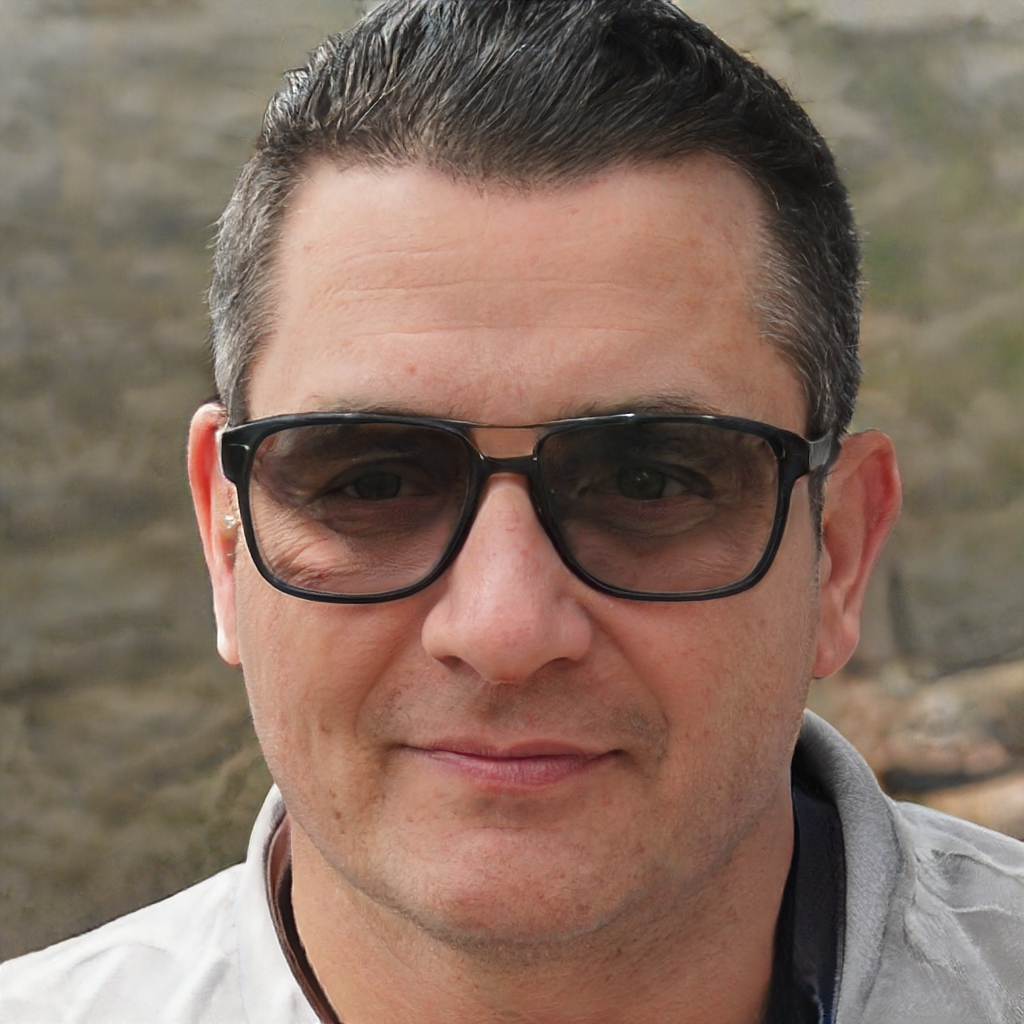
\includegraphics[height=3cm]{imagenes/Persona2.jpg}
				\end{center}
			\end{minipage}
		}                 \\ [2ex]
		\cline{1-2}
		Edad         & 46 &                                   \\ [2ex] 
		\cline{1-2}
		Género         & Masculino &                                   \\ [2ex]
		\cline{1-2}
		Profesión    & 
			\begin{minipage}[t]{0.3 \textwidth}
				Funcionario
			\end{minipage}
		 &                                   \\ [2ex] 
		\hline
		\multicolumn{3}{|l|}{{\cellcolor{lightblue}}\textbf{Contexto de uso}}               \\ 
		\hline
		Cuándo       & \multicolumn{2}{l|}{Al llegar a casa}                \\ 
		\hline
		Dónde        & \multicolumn{2}{l|}{Ordenador portátil y/o aparato dedicado}                \\ 
		\hline
		\multicolumn{3}{|l|}{{\cellcolor{lightblue}}\textbf{Misión}}                        \\ 
		\hline
		Objetivo     & \multicolumn{2}{l|}{Poder disfrutar de cierta independencia}                \\ 
		\hline
		Expectativas & \multicolumn{2}{l|}{
			\begin{minipage} [t] {0.7\textwidth}
				\begin{itemize}
					\item Permitir escuchar alguna información proveniente de Internet (Noticias, Tiempo...)
					\item Escuchar música, podcasts...
				\end{itemize}
			\end{minipage}
		}                \\ 
		\hline
		\multicolumn{3}{|l|}{{\cellcolor{lightblue}}\textbf{Motivación}}                   \\ 
		\hline
		Urgencia     & \multicolumn{2}{l|}{
			\begin{minipage}[t]{0.7\textwidth}
				No le sería de mucha urgencia, pero le encantaría tenerlo cuanto antes
			\end{minipage}
		}                \\ 
		\hline
		Deseo        & \multicolumn{2}{l|}{
			\begin{minipage}[t]{0.7\textwidth}
				Desde que perdió parcialmente la visión, no ha podido volver a dedicarse a pasiones como la literatura de forma fácil (por ejemplo, teniendo que esperar bastante tiempo para obtener audiolibros o libros adaptados a braille) o informarse en cualquier momento sin tener que pasar por el ordenador adaptado.
			\end{minipage}
		}                \\ 
		\hline
		\multicolumn{3}{|l|}{{\cellcolor{lightblue}}\textbf{Actitud ante la tecnología}}    \\ 
		\hline
		\multicolumn{3}{|l|}{
			\begin{minipage}[t]{\textwidth}
				Apenas usa el ordenador para alguna que otra gestión del trabajo.
			\end{minipage}
		}                              \\
		\hline
	\end{tabular}
	\caption[Ficha Persona 2]{Ficha de la Persona 2 (Javier Pedrosa). Imagen extraída de \cite{thispersondoesnotexist}}
\end{table}

\newpage

\section{Casos de uso: ¿Qué podrían hacer?}

Una vez pensado en posibles perfiles de uso, podríamos preguntarnos por alguna incidencia que pudiera solucionarse o facilitarse gracias al sistema resultante.

Los casos de uso en las metodologías ágiles nos permiten, a partir de las personas expuestas anteriormente, promover casos y analizarlos para encontrar posibles causísticas donde se pueda ver alguna inconformidad con el sistema resultante para tratar de paliarlo y prevenirlo en la fase de análisis.

\subsection{Caso 1: Irene y el calendario de exámenes}

Para nuestra primera persona podemos tener el siguiente caso:

`` \textit{5 de Abril de 2022. Se acerca la época de exámenes finales y poco a poco Irene va teniendo las fechas de estos. Viendo que es el momento de ponerse a prepararlos, apunta todos en su agenda, pero como en esta tiene además las tareas que ha de realizar, decide apuntar esos exámenes en el teléfono y en una hoja de calendario que tendrá que imprimir en la librería de al lado de su casa.}

\textit{Al llegar a casa, coge el teléfono y los va anotando. Además, descarga un PDF con el calendario del mes y llega a la tienda para imprimirlos. Al volver, también los anota, aunque con algo de prisa para ponerse a hacer las tareas que tenía que terminar para mañana. En el descuido los deja en un estante mal colocados y se caen al suelo mojado tras fregar la habitación, dejando la tinta borrosa.}

\textit{Al verlo, Irene se enfada un tanto por tener que volver a hacer el calendario.} ''

\textbf{¿Cómo se podría entonces solucionar este problema?} Podríamos aplicar el Asistente a través de una conversación donde se podría comunicar las fechas con tal de crear recordatorios o consultar a través de la voz si tiene algún evento en los próximos días.

Podríamos así tener una conversación para cada examen que quisiera introducir similar a:

\textit{
	\begin{itemize}
		\item \textbf{Irene}: Recuérdame que tengo examen de Historia de España el 22 de Abril.
		\item \textbf{Bot}: De acuerdo, el 22 de Abril te recordaré ``Examen de Historia de España''
	\end{itemize}
}

\subsection{Caso 2: Irene y la técnica Pomodoro}

Continuando con nuestra primera persona, podríamos darnos con otro caso en el que integrar el software podría servirle de ayuda.

`` \textit{15 de Abril de 2022. Una semana para el examen de Historia de España. Irene va a su cuarto con su reloj y prepara un temporizador de 25 minutos.}

\textit{Mientras estudia, se queda tan centrada que pasa al tiempo de descanso sin notar que el reloj ha vibrado. Cuando mira el reloj, se había pasado media hora más, así que se piensa hacer los 5 minutos de descanso en ese momento antes de activar el temporizador otra vez. Pero en ese caso tenía que estar pendiente del tiempo para no pasarse.} 

\textit{El día acabó siendo bastante fructífero y había preparado sus apuntes para poder seguir estudiando al día siguiente, pero fue un tanto molesto para ella ya que estar pendiente del reloj era un poco engorroso.}''

\textbf{¿Cómo se podría entonces solucionar este problema?} Podríamos aplicar el Asistente a través de dos cuentas atrás, una para la parte de estudio y otra para la parte de descanso, y pedir verbalmente que lo repita X veces, o que simplemente a través de pedir que ponga un contador Pomodoro se genere una conversación para configurar los tiempos y activarse automáticamente.

Podríamos así tener dos estilos de conversación:

La primera opción, que se repitiría tres veces:
\textit{
	\begin{itemize}
		\item \textbf{Irene}: Bot, ponme un contador de 25 minutos
		\item \textbf{Bot}: Contador en marcha
		\item \textbf{Bot}: *Suena alarma*
		\item \textbf{Irene}: Bot, ponme un contador de 5 minutos
		\item \textbf{Bot}: Contador en marcha
		\item \textbf{Bot}: *Suena alarma*
	\end{itemize}
}

La segunda opción, donde se configuraría una vez:
\textit{
	\begin{itemize}
		\item \textbf{Irene}: Bot, activa el contador Pomodoro
		\item \textbf{Bot}: Ok, ¿cuánto tiempo quieres ponerte a estudiar?
		\item \textbf{Irene}: 25 minutos
		\item \textbf{Bot}: De acuerdo. ¿Cuántos de descanso?
		\item \textbf{Irene}: 5 minutos
		\item \textbf{Bot}: Vale. ¿Y cuántas veces?
		\item \textbf{Irene}: Tres.
		\item \textbf{Bot}: De acuerdo. El tiempo de estudio comienza en 3,2,1... ¡Tiempo!
		\item \textbf{Bot}: (Tras 25 minutos) 3,2,1... ¡Es hora de un descanso!
		\item \textbf{Bot}: (Tras 5 minutos) 3,2,1... ¡Manos a la obra de nuevo!
		\item \textbf{Bot}: (Tras 25 minutos a la tercera vez) 3,2,1... *Alarma*
	\end{itemize}
}

\subsection{Caso 3: Javier y las noticias}

Para nuestra segunda persona, podríamos crear un caso en base a su condición especial:

``
\textit{Javier está sentado en el sofá escuchando la señal del canal de Noticias 24h cuando le llega un mensaje sobre una noticia de su pueblo. Quiere ir a leerlo pero el lector del teléfono se pone a leer partes de anuncios y se exaspera un tanto.}

\textit{Buscando otra alternativa, se pone en el ordenador con el visor Braille. Intentando abrir la noticia, debe teclearla letra a letra, incomodándose un poco. Finalmente, tras una pequeña odisea, logra digitar la noticia y enterarse de que un amigo de la infancia había salido en portada por un logro en el que había participado.}
''

\textbf{¿Cómo se podría entonces solucionar este problema?} Podríamos aplicar el Asistente a través de una conversación donde se podría poner a leer las noticias de un diario.

Podríamos así tener una conversación para cada examen que quisiera introducir similar a:

\textit{
	\begin{itemize}
		\item \textbf{Javier}: Bot, ¿podrías leerme las noticias del diario <Diario>?
		\item \textbf{Bot}: De acuerdo, aquí hay una noticia que dice así: ``Detenidos 2 vándalos que han pintado un tren del Metropolitano de Granada''. ¿Sigo leyendo?
		\item \textbf{Javier}: Siguiente.
		\item \textbf{Bot}: Vale, aquí hay otra noticia: ``Científicos de la UGR logran crear una memoria con materiales reciclados''. ¿Sigo leyendo?
		\item \textbf{Javier}: Si.
	\end{itemize}
}

En general, de los 3 casos podríamos sacar, sin entrar en las particularidades de cada caso:
\begin{enumerate}
	\item El sistema debe permitir una modularidad de forma que se puedan añadir nuevas funcionalidades sin necesidad de tocar todo el código principal.
	\item Habría que tener en cuenta el contexto donde se esté conversando, ya que no es lo mismo cuando le llega una orden durante una conversación que nada más activar la \textit{trigger word}
	\item Las respuestas deben sonar lo más claras y concisas posible.
	\item Las órdenes deberían tener cierta flexibilidad en su forma de expresarse, ya que para pedir, por ejemplo, que se inicie un temporizador, podríamos decir \textit{Activa un temporizador para dentro de X minutos} o \textit{Programa una cuenta atrás de X minutos}
\end{enumerate}


\begin{table}[H]
	\centering
	\begin{tabularx}{\textwidth}{|>{\columncolor{mintgreen}}c>{\columncolor{mintgreen}}X|}
		\hline
		
\includegraphics[width=30pt]{imagenes/Tarea_completada.png} & Con ello, cumplimos el Objetivo \textbf{O-DD 1.} (Diseñar personas y casos de uso en los que el software podría presentar algún problema con tal de buscar soluciones o limitaciones.) \\
		\hline
	\end{tabularx}
\end{table}

\section{Análisis competitivo}

Otra manera de encontrar posibles requisitos es observando a la competencia. Para ello podríamos analizar la funcionalidad de algunos de los competidores y sacar elementos comunes que podríamos traer en nuestro proyecto.

Para el análisis compararemos los siguientes proyectos, los cuales están mencionados en el capítulo 3 sobre el estado del arte:

\begin{itemize}
	\item \textbf{Amazon Alexa} \cite{alexa}, a través de un dispositivo Echo Dot previamente configurado para obtener señal de Internet y conectado a una aplicación en el teléfono a través de la cual se ha iniciado sesión con una cuenta de Amazon.
	\item \textbf{Microsoft Cortana} \cite{cortana}, a través de un ordenador con el Sistema Operativo Windows 10 instalado, y habiendo iniciado sesión previamente (pues es requerido por el programa)
	\item \textbf{Google Assistant} \cite{google-assistant}, a través de un teléfono móvil Android que se use a diario. Téngase en cuenta que para poder usar estos dispositivos se requiere tener una cuenta de Google.
\end{itemize}

Nótese que en el análisis queda fuera \textbf{Apple Siri} \cite{siri} ya que para ello requeriríamos de un dispositivo del ecosistema de Apple, y a fecha del análisis no se tenía en posesión de ningún dispositivo de la compañía.
\newpage

%\begin{xltabular}[H]
	\begin{xltabular}{\textwidth}{|c|X|X|X|}
		
		\hline \multicolumn{4}{|r|}{{Continúa en la siguiente página $>>$}} \\ \hline
		\endfoot
		
		\hline
		\endlastfoot
		
		\hline
		{\cellcolor{mintgreen}} \textbf{\textit{Propiedad}} & {\cellcolor{mintgreen}} \textbf{Alexa} & {\cellcolor{mintgreen}} \textbf{Cortana} & {\cellcolor{mintgreen}} \textbf{G-Assistant} \\
		\hline
		\textit{¿Dónde se puede usar?} & En dispositivos Echo y en la app Alexa & En ordenadores con Windows 10 y teléfonos Android y Apple & En teléfonos Android y en la web, además de dispositivos Google Home. \\
		\hline
		\begin{minipage}[t]{0.3\textwidth}
			\textit{¿Qué se necesita para empezar a usarlo?}
		\end{minipage} & Cuenta de Amazon y acceso a Internet & Acceso a Internet. Últimamente, cuenta de Microsoft. & Cuenta de GMail/Google y acceso a Internet.\\
	    \hline
	    \multirow{2}{*}{\begin{minipage}[t]{0.3\textwidth}
	    		\textit{¿Se puede añadir funcionalidades?¿Cómo?}
	    \end{minipage}}
	     & Se pueden programar \textit{skills} para distintos propósitos. Se puede descargar desde la app de Alexa. & Se podía, pero su creación ha quedado depreciada & Se permite a través del SDK de Google Actions. Se puede preguntar a la skill en concreto, aunque tiene su catálogo también para poder instalarlos\\
	     \cline{2-4}
         & \multicolumn{3}{c|}{\begin{minipage}[t]{0.6\textwidth}
        		En algunas skills habrá que tener en cuenta que se requiera iniciar sesión en alguna cuenta de terceros
        	\end{minipage}} \\
        \hline
        \begin{minipage}[t]{0.3\textwidth}
        	\textit{¿Cómo es el comportamiento en caso de que falle el Internet?}
        \end{minipage} & Avisa de que falta la conexión a Internet, pero reconoce la palabra clave & Al pulsar en el programa no contesta, pero informa de que no hay conexión & Al pulsar en el programa no contesta, pero informa de que no hay conexión\\
        \hline
        \begin{minipage}[t]{0.3\textwidth}
        	\textit{¿El asistente puede reconocer varias maneras de decir una misma frase?}
        \end{minipage} & Sigue ciertos patrones, y según la función permite cambiar la manera de expresar la orden o no & Tiene unas estructuras más fijas, no da mucho margen a expresar las órdenes de otra forma & Para funciones propias tiene una mayor variedad de patrones, pero para invocar las realizadas por otros se usa un patrón fijo \\ 
        \hline
        \begin{minipage}[t]{0.3\textwidth}
        	\textit{¿El asistente puede responder de varias maneras a una orden?}
        \end{minipage} & Para funciones que pueden cambiar en cualquier momento (por ej. Pedir la hora), suele tener una parte que no cambia, y según la función, añade ciertas frases. En otras órdenes, responde de forma aleatoria una respuesta de su repertorio. Si sólo tiene una, será esa la que se reproduzca & Responde de forma aleatoria una respuesta de su repertorio, o la única que tiene & Responde de forma aleatoria una respuesta de su repertorio, o la única que tiene \\ 
        \hline
	\caption{Análisis competitivo entre Alexa, Cortana y Google Assistant}
	\end{xltabular}
	
%\end{xltabular}

\begin{table}[H]
	\centering
	\begin{tabularx}{\textwidth}{|>{\columncolor{mintgreen}}c>{\columncolor{mintgreen}}X|}
		\hline
		
\includegraphics[width=30pt]{imagenes/Tarea_completada.png} & Con ello, cumplimos el Objetivo \textbf{O-IA 3.} (Analizar desde un punto de vista competitivo las prestaciones que ofrecen otras alternativas propietarias y libres (si las hay)) \\
		\hline
	\end{tabularx}
\end{table}

\section{La Ingeniería de Requisitos en acción}

\subsection{Requisitos funcionales}
A continuación se listarán aquellos requisitos que se requerirán para realizar el Asistente de Voz a un nivel de Producto Mínimo Viable. Esto no quiere decir que se puedan añadir más funcionalidades en un futuro. De haber más, se indicarán a lo largo del documento.

\begin{table}[H]
	\centering
	\begin{tabularx}{\textwidth}{|c|X|} 
		\hline
		\textbf{Nº de RF }          &  1 \\ 
		\hline
		\textbf{Nombre}         &  Hablar al Asistente \\ 
		\hline
		\textbf{Descripción}    &  Como usuario, quiero poder hablar con el programa para comunicarme con este \\ 
		\hline
		\textbf{Prioridad}      &  Alta  \\ 
		\hline
		\textbf{Entrada}        & Un sonido  \\ 
		\hline
		\textbf{Prerrequisitos} & Debe ser un audio hablado con la compresión que requiera las APIs que intervengan  \\ 
		\hline
		\textbf{Procesamiento}  &  Envía el audio para que el computador lo pueda entender \\ 
		\hline
		\textbf{Postcondición}  &  - \\
		\hline
	\end{tabularx}
	\caption{Descripción del Requisito Funcional 1: Hablar al Asistente}
\end{table}

\begin{table}[H]
	\centering
	\begin{tabularx}{\textwidth}{|c|X|} 
		\hline
		\textbf{Nº de RF }          &  2 \\ 
		\hline
		\textbf{Nombre}         &  Escuchar una respuesta del Asistente \\ 
		\hline
		\textbf{Descripción}    &  Como usuario, quiero poder escuchar la respuesta del programa para comunicarme con este \\ 
		\hline
		\textbf{Prioridad}      &  Alta  \\ 
		\hline
		\textbf{Entrada}        & Un sonido  \\ 
		\hline
		\textbf{Prerrequisitos} & La respuesta ha debido ser generada para poder pronunciarla \\ 
		\hline
		\textbf{Procesamiento}  &  Se generará un audio leyendo la respuesta conforme a los requisitos de la API que se use para reproducir el sonido. \\ 
		\hline
		\textbf{Postcondición}  &  - \\
		\hline
	\end{tabularx}
	\caption{Descripción del Requisito Funcional 2: Escuchar al Asistente}
\end{table}

\begin{table}[H]
	\centering
	\begin{tabularx}{\textwidth}{|c|X|} 
		\hline
		\textbf{Nº de RF }          &  3 \\ 
		\hline
		\textbf{Nombre}         &  Sintetizar la voz de una pregunta \\ 
		\hline
		\textbf{Descripción}    &  Como sistema, quiero poder leer la pregunta para comunicarme con el usuario \\ 
		\hline
		\textbf{Prioridad}      &  Alta  \\ 
		\hline
		\textbf{Entrada}        & Un sonido grabado  \\ 
		\hline
		\textbf{Prerrequisitos} & Debe ser un audio hablado con la compresión que requiera las APIs que intervengan \\ 
		\hline
		\textbf{Procesamiento}  &  A través de un algoritmo de Speech Recognition, convertir el audio en un texto \\ 
		\hline
		\textbf{Postcondición}  &  - \\
		\hline
	\end{tabularx}
	\caption{Descripción del Requisito Funcional 3: Sintetizar la voz de una pregunta.}
	\vspace{0.5cm}
	\centering
	\begin{tabularx}{\textwidth}{|c|X|} 
		\hline
		\textbf{Nº de RF }          &  4 \\ 
		\hline
		\textbf{Nombre}         &  Generar un audio con la respuesta \\ 
		\hline
		\textbf{Descripción}    &  Como sistema, quiero poder hablar la respuesta del programa para comunicarme con el usuario \\ 
		\hline
		\textbf{Prioridad}      &  Alta  \\ 
		\hline
		\textbf{Entrada}        & Una cadena de texto con la respuesta  \\ 
		\hline
		\textbf{Prerrequisitos} & - \\ 
		\hline
		\textbf{Procesamiento}  &  A través de un algoritmo de Text-To-Speech, convertir el texto en un audio \\ 
		\hline
		\textbf{Postcondición}  &  - \\
		\hline
	\end{tabularx}
	\caption{Descripción del Requisito Funcional 4: Generar un audio con la respuesta.}
	\vspace{0.5cm}
	\centering
	\begin{tabularx}{\textwidth}{|c|X|} 
		\hline
		\textbf{Nº de RF }          &  5 \\ 
		\hline
		\textbf{Nombre}         &  Relacionar una pregunta con una respuesta  \\ 
		\hline
		\textbf{Descripción}    &  Como sistema, quiero procesar la pregunta para poder ofrecer una respuesta \\ 
		\hline
		\textbf{Prioridad}      &  Alta  \\ 
		\hline
		\textbf{Entrada}        & Una cadena de texto con la respuesta  \\ 
		\hline
		\textbf{Prerrequisitos} & - \\ 
		\hline
		\textbf{Procesamiento}  &  Buscará a través de un patrón o similar una respuesta a la petición del usuario \\ 
		\hline
		\textbf{Postcondición}  &  - \\
		\hline
	\end{tabularx}
	\caption{Descripción del Requisito Funcional 5: Relacionar una pregunta con una respuesta.}
\end{table}


\begin{table}[H]
	\centering
	\begin{tabularx}{\textwidth}{|c|X|} 
		\hline
		\textbf{Nº de RF }          &  6 \\ 
		\hline
		\textbf{Nombre}         &  Avisar que no se puede conectar a Internet  \\ 
		\hline
		\textbf{Descripción}    &  Como sistema, quiero comunicar que no se ha podido conectar a Internet para que el usuario trate de arreglar la incidencia \\ 
		\hline
		\textbf{Prioridad}      &  Media  \\ 
		\hline
		\textbf{Entrada}        & - \\ 
		\hline
		\textbf{Prerrequisitos} & Se ha tenido que generar una pregunta previa que requiriese usar servicios en línea  \\ 
		\hline
		\textbf{Procesamiento}  &  Generará un audio para avisar que no se puede conectar \\ 
		\hline
		\textbf{Postcondición}  &  - \\
		\hline
	\end{tabularx}
	\caption{Descripción del Requisito Funcional 6: Avisar que no se puede conectar a Internet}
\end{table}

\begin{table}[H]
	\centering
	\begin{tabularx}{\textwidth}{|c|X|} 
		\hline
		\textbf{Nº de RF }          &  7 \\ 
		\hline
		\textbf{Nombre}         &  Responder que se desconoce la respuesta  \\ 
		\hline
		\textbf{Descripción}    &  Como sistema, quiero poder comunicar que no sé la respuesta a la pregunta para poder avisar al usuario \\ 
		\hline
		\textbf{Prioridad}      &  Media  \\ 
		\hline
		\textbf{Entrada}        & -  \\ 
		\hline
		\textbf{Prerrequisitos} & La pregunta dicha anteriormente no coincide con algún patrón o tipo de pregunta \\ 
		\hline
		\textbf{Procesamiento}  &  Generará un audio para responder al usuario \\ 
		\hline
		\textbf{Postcondición}  &  - \\
		\hline
	\end{tabularx}
	\caption{Descripción del Requisito Funcional 7: Responder que se desconoce la respuesta}
\end{table}

\subsection{Requisitos no funcionales}

\begin{enumerate}[\textbf{RNF-} 1.]
	\item \textbf{Usabilidad y legibilidad del código:} Debido a que va a ser un proyecto que luego se publicará y que además da pie a que otras personas colaboren en él, sería conveniente que el código sea lo más claro y conciso posible. Por tanto:
	\begin{itemize}
		\item Se realizará una \textbf{codificación modular}, de forma que los cambios estén lo más localizados posible y que no se requieran hacer muchos de ellos.
		\item El código deberá seguir los estándares y convenios de codificación del lenguaje \textbf{Python}. Para comprobarlo, usaremos como linter \textbf{PyLint} \cite{pylint}, ya que nos aconsejará y advertirá tanto de posibles errores lógicos como de código que haya que refactorizar para seguir esos estándares.
	\end{itemize}

	\item \textbf{Implementación:} Para realizar el proyecto, haremos uso de varias tecnologías. Principalmente, requeriremos:
		\begin{itemize}
			\item Como lenguaje de programación principal se usará una versión >=3.5 de \textbf{Python}.
			\item Se usarán APIs y Frameworks de Reconocimiento de Voz y de Text-to-Speech que posean licencias de \textbf{Software Libre} (GPL/LGPL/AGPL) o de \textbf{Código Abierto} (Licencia Apache/Mozilla/BSD).
			\item De la misma manera, aquellos Frameworks que persigan la relación entre las preguntas o peticiones del usuario y las respuestas del sistema deberán seguir esas mismas condiciones.
			\item En consecuencia, la versión de Python a utilizar deberá ser la última que soporten todas sus dependencias.
		\end{itemize}
	
	\item \textbf{Rendimiento}: Al ser un sistema que requiere una interacción con el usuario lo más fluida posible, tendremos que regir alguna restricción:
	\begin{itemize}
		\item El tiempo entre la pregunta y la respuesta no debería exceder de los 5 segundos.
	\end{itemize}

	\item \textbf{Información a utilizar}: Al ser un sistema que interactúa con el usuario, recogerá algunos datos sensibles como nombre, IP del dispositivo donde está instalado o la propia voz. Por tanto:
	\begin{itemize}
		\item Los datos que se usen para personalizar la experiencia no deberán ser enviados, a no ser que se requiera alguna conexión a Internet, en cuyo caso se daría sólo lo necesario (por ejemplo, si se registra un lugar para consultar el tiempo, sólo se debería enviar una petición para consultar esa información para ese lugar).
		\item El \textbf{tratamiento de la voz}, de ser posible, se realizará \textbf{en el propio dispositivo}.
		\item Si se requiriera enviar alguna información sensible más allá de lo contemplado, debería de al menos \textbf{notificarse} una vez al usuario (por ejemplo, en la configuración inicial o en la documentación).
	\end{itemize}
.
	\item \textbf{Ámbito legal}: Al ser un sistema que usa ciertas dependencias con licencias, sería necesario regularizar la situación con el siguiente requisito:
	\begin{itemize}
		\item La licencia del proyecto resultante deberá ser \textbf{compatible} con todas las dependencias utilizadas en este.
	\end{itemize}

	\item \textbf{Sistema}: El proyecto resultante debe poder ejecutarse en al menos algún dispositivo. Por tanto, las \textbf{características} del sistema a utilizar serían:
	\begin{itemize}
		\item Con \textbf{entrada y salida de audio}, bien soldado o cableado, bien a través de conectores (como Jack)
		\item Capaz de \textbf{ejecutar} la versión de \textbf{Python} y las dependencias asociadas
	\end{itemize}

	De cara al desarrollo usaremos dos dispositivos para poder probarlo:
	\begin{itemize}
		\item El \textbf{portátil} donde se desarrollará el proyecto.
		\item Una \textbf{Raspberry Pi 3B}, que tratará de emular a los dispositivos dedicados vistos en el Análisis Competitivo.
	\end{itemize}
	Estos usarán una distribución de \textbf{Linux} (\textit{Kubuntu 20.04} en el caso del portátil y \textit{Raspberry Pi OS} en el caso del dispositivo homónimo) siguiendo los requisitos de Implementación.
\end{enumerate}
 
	
	\newpage 
	\chapter{Planificación}

\noindent\fbox{
	\parbox{\textwidth}{
		En este apartado realizaremos una estimación del tiempo necesario para realizar el proyecto, y cuantificaremos las tareas que se deberían cumplir, acabando con un diagrama de Gantt que contará gráficamente el tiempo empleado en realizarlos aproximadamente.
	}
}

\section{Metodología utilizada}
Para desarrollar el proyecto se ha optado por una Metodología Ágil basada en SCRUM, ya que permite mucha flexibilidad temporal y mayor control en las tareas que hay que realizar. Además, si hay alguna tarea que se debe añadir durante el desarrollo, se puede introducir al backlog y tratarlo posteriormente.

\section{Temporización}
A grandes rasgos, se han desarrollado los objetivos separándolos en acciones más pequeñas para poder cumplirlas. En el análisis se terminarán de definir todas las tareas con tal de poder tener un Product Backlog definido totalmente para poder desarrollar todo lo necesario.

\subsection{El Product Backlog}

\subsection{División en sprints}
Un primer esbozo para dividir todas las tareas en 3 grandes sprints de forma que se vayan realizando de forma continua y constante.

\subsubsection{Sprint 1: ( semanas)}

\subsubsection{Sprint 2: ( semanas)}

\subsubsection{Sprint 3: ( semanas)}

\subsection{Diagrama de Gantt}
La temporización en este punto quedaría desarrollada por el siguiente Diagrama de Gantt:


\section{Seguimiento del desarrollo}
Para seguir el desarrollo se hará uso de dos artefactos que acompañan al framework SCRUM:
\begin{itemize}
	\item Sprint Backlogs : Al principio de cada Sprint se revisará si queda alguna tarea pendiente y si hay que recalcular algo. Como base tendremos los de la subsección 5.2.1
	\item Gráfica de Burndown: Cada vez que se termine una tarea se actualizará esta gráfica.
\end{itemize}

\section{Estimación de costes}
\subsection{El personal}
Si bien este proyecto se va a acabar realizando por una persona realmente, supongamos el caso de que este proyecto lo realizara una pequeña startup de 4 miembros, de forma que hubiera un Scrum Master, un Product Owner, un documentalista y un desarrollador que trabajará principalmente en Python.

\subsection {Costes de productos físicos}
En el inventario hardware del proyecto se usarían dos dispositivos principalmente: Un ordenador portátil donde se desarrolle y pruebe el proyecto, y una Raspberry Pi 3B para las pruebas que se quieran hacer.

Listamos en la siguiente tabla los costes relacionados con ellos:

\subsection{Costes de productos lógicos}
En el caso de las herramientas software, notamos que todas son gratuitas, pero debido a que son unas cuantas y con propósitos variados, vemos interesante desglosarlos.




	% Análisis del problema
	% 1. Análisis de requisitos
	% 2. Análisis de las soluciones
	% 3. Solucion propuesta
	% 4. Análisis de seguridad
	\newpage 
	\chapter{Análisis del problema}

\noindent\fbox{
	\parbox{\textwidth}{
		En el capítulo se analizan las herramientas para preparar el diseño del proyecto de cara a su posterior codificación.
	}
}

\section{Comparando APIs de Reconocimiento de Voz}
\subsection{Introducción}
Como hablamos en el Capítulo 2, hoy en día existen herramientas que reconocen la voz. Algunas son de software propietario o de Software como Servicio (por ejemplo, IBM Watson SR o Google SR), pero también hay proyectos de software de código abierto que nos permiten trabajar con ello sin tener que saber los tópicos de la Inteligencia Artificial a fondo, trabajando de forma transparente al desarrollador. 

Entre estos proyectos podemos encontrar dos:
\begin{itemize}
	\item \textbf{Vosk API \cite{vosk}}:Desarrollado por Alpha Cephei en 2019 como wrapper de Kaldi , es un sistema de Reconocimiento de Voz offline que actualmente soporta 17 lenguajes y destaca por funcionar en dispositivos más limitados como la Raspberry Pi. Sus modelos más básicos son de 50 MB, pero se pueden adaptar a modelos más complejos, consiguiendo así una escalabilidad en el sistema. Además, soporta reconocimiento del habla. En su arquitectura se usa una red neuronal en conjunto con un Modelo Oculto de Markov. Usa una licencia Apache 2.0
	
	\item \textbf{Mozilla DeepSpeech \cite{deepspeech}}: Es una API de Reconocimiento de Voz realizado por Mozilla desde 2016, basado en un paper de Baidu sobre un sistema de Reconocimiento del Habla usando algoritmos de Deep Learning en conjunto con optimizaciones para lograr resultados más rápidos usando múltiples GPU para alimentar una Red Neuronal Recurrente que modelizara un lenguaje en base a ingentes cantidades de datos. Por tanto, acaban dando en la API una interfaz para poder usarlo en nuestros ordenadores y una serie de modelos optimizados gracias al entrenamiento que pueden realizar.
	
\end{itemize}

\subsection{Experimentos}

Para saber cuál sería la API que más nos interesara, podríamos montar un experimento donde evaluaríamos:
\begin{itemize}
	\item La facilidad de implementación
	\item La precisión de los modelos y de la API.
\end{itemize}

Este experimento se basaría en coger a varios sujetos que leyeran un mismo texto.
Esas lecturas se pasarían por un programa que emplea la API de forma que acabamos convirtiendo la voz en texto. Tras ello, se comparan ambos textos para ver el \textbf{Word Error Rate (WER)} \cite{wer-cer}, una métrica que mide la precisión entre lo que se ha querido decir y lo que un Reconocedor del Habla transcribe. 

El algoritmo del Word Error Rate consiste en mapear dos cadenas de texto (una indica qué se quiere decir y la otra es lo que se ha detectado) para extraer las diferencias (palabras \textbf{\textit{I}}ntroducidas, \textbf{\textit{S}}ustituidas o \textbf{\textit{R}}etiradas)  y medirlas respecto al \textbf{\textit{N}}úmero total de palabras del texto. Por tanto, su fórmula sería:

\begin{equation}
	WER = \frac{I+S+R}{N}
\end{equation}

También estaría interesante fijarnos en el CER (Character Error Rate) \cite{wer-cer} para ver también a nivel de caracteres qué errores se pueden encontrar en la transcripción (por ejemplo, los acentos). La fórmula sería la misma pero las inserciones, sustituciones y eliminaciones se observan letra a letra.

\begin{equation}
	CER = \frac{I_c+S_c+R_c}{N_c}
\end{equation}

Nos quedaríamos entonces con aquella implementación que sea más fácil de usar en conjunto con el modelo más preciso. 

Otra cosa que también podemos probar, de paso, es decir varios nombres propios con tal de mirar si le podemos poner nombre al Asistente, pues hoy en día es común usar como \textit{trigger word} un nombre propio (como \textit{Alexa}, \textit{Siri} o \textit{Cortana}). También podemos probar a decir acciones que debería reconocer el asistente habitualmente para funcionalidades futuras, incluso probar a decir cosas en otros idiomas (por ejemplo, canciones con títulos en inglés) para ver cómo reacciona.

Así pues, se ha redactado el siguiente texto para hacer las pruebas:

\noindent\fbox{
	\parbox{\textwidth}{
		Lúmina y Arcadia se encuentran en un portal a medio camino entre sus casas, cerca del centro comercial. Ellas habían quedado para ver la nueva película que tanto promocionaban por la tele y buscaron un momento entre sus agendas para ir a verla. 
		
		Lumi comparte uno de sus auriculares con su amiga y  enciende el móvil. Entra a Spotify y reproduce un tema de Katy Perry mientras pasean hacia su destino.
		
		Al llegar, buscan el cine y compran las entradas y las palomitas. Al entrar a la sala ven un temporizador de 5 minutos en la pantalla, que además no paraba de poner publicidad.
		
		De repente, todo se para por un corte de luz. Todo estaba a oscuras y alguien enciende la luz de su teléfono, aunque no sirve de mucho hasta que vuelve el suministro a funcionar y ya puedan ver la película.
		
		Al terminar, miran qué tiempo hace para saber si esperar a que les recojan o volver andando. Aunque lo piensan mejor tras mirar qué hora es y deciden ir a tomar un café antes de irse.
	}
}

Además de este texto tan largo, se ha probado a hacer audios más cortos, ya que suelen estar entrenados con segmentos de pocos segundos, a modo de órdenes:

\noindent\fbox{
	\parbox{\textwidth}{
		Enciende la luz.
		
		Ponme esa canción que tanto me gusta.
		
		Repite lo que diga.
		
		Para.
		
		Espera un momento.
		
		Reproduce el informativo de la mañana.
		
		Ponme una alarma a las ocho y media de la mañana.
		
		Prepara un temporizador de 5 minutos.
	}
}

De cada frase se preparará un par de variantes, ya que queremos ver cómo se comportan al nombrar varias propuestas de nombre para el producto. Estos nombres serían Arcadia y Lúmina.

En primera instancia, los cuales han grabado su voz durante la lectura. Se ha comprobado previamente de forma manual que lo que se oye es exactamente lo que se lee, ya que podría ocasionar cierto ruido el hecho de que no fuera así. Tras ello se ha tratado el audio con cada uno de los modelos y configuraciones.

En el caso de Vosk, acabaremos extrayendo su WER y CER para cada uno de los audios según su modelo oficial.

Para el caso de DeepSpeech, se ha trabajado con dos modelos ya entrenados y dos scorers, combinando ambos parámetros.

Los modelos que se probarán son:
\begin{itemize}
	\item \textbf{Polyglot} \cite{scribosermo}: Este modelo fue entrenado por un usuario de la Comunidad de Mozilla, entrenando un set de 812 horas con GPUs de Nvidia \cite{scribosermo}. Usa una licencia LGPL versión 3.
	\item \textbf{Rhasspy}: Este modelo estaba pensado para usarse en otro sistema de asistente de voz con una Raspberry Pi, basado en una versión anterior del modelo descrito anteriormente.
\end{itemize}

En el mismo modelo Polyglot, se nos daban dos scorers. Un scorer es un complemento del modelo del lenguaje que permite predecir qué palabra sigue. En este caso, se ha decidido usar dos para ver si causaban alguna diferencia:

\begin{itemize}
	\item \textbf{Ken}: Es un scorer ligero, con poco entrenamiento.
	\item \textbf{Poco} : Es un scorer pesado pero más completo.
\end{itemize} 

DeepSpeech también admitía dos valores extra: Alfa y Beta. Estos parámetros definen el peso del modelo del lenguaje y cuánto se penaliza por introducir una palabra. Para tener un abanico de opciones, para cada combinación se ha tratado de buscar un valor óptimo para estos parámetros, con la precisión de una décima, en un rango de 1 a 2 para el valor Alfa (a mayor valor, más importancia le dará a seguir el modelo) y un rango de 0 a 1 para el valor Beta (a mayor valor, más penalización sufrirá por una transcripción errónea).

Este experimento se repetirá 3 veces usando al mismo locutor con las mismas frases.

\subsection{Resultados}

Tras realizar los experimentos se ha notado que devuelven los mismos valores, agrupándolos en esta tabla:

{\small\tabcolsep=2pt\setlength\LTleft{-35pt}	
	\begin{xltabular}{\textwidth}{|ll|l|llll|}
		\hline \multicolumn{4}{|r|}{{Continúa en la siguiente página $>>$}} \\ \hline
		\endfoot
		
		\hline
		\endlastfoot
		
		\hline
		\multicolumn{2}{|l|}{\multirow{3}{*}{}}                           & \multirow{3}{*}{\textbf{Vosk}} & \multicolumn{4}{c|}{\textbf{DeepSpeech}}                                                                                   \\ \cline{4-7} 
		\multicolumn{2}{|l|}{}                                            &                                & \multicolumn{2}{c|}{Modelo Rhasspy}                                    & \multicolumn{2}{c|}{Modelo Polyglot}              \\ \cline{4-7} 
		\multicolumn{2}{|l|}{}                                            &   
		   & \multicolumn{1}{l|}{Scorer PocoLG} & \multicolumn{1}{l|}{Scorer KenLM} & \multicolumn{1}{l|}{Scorer PocoLG} & Scorer KenLM \\ \hline
		\multicolumn{1}{|l|}{\textbf{Texto Largo}}              &         & \makecell{\textbf{CER = 0,1189} \\ \textbf{WER = 0,2944}}  & \multicolumn{1}{l|}{\makecell{$\alpha$ = 1,2/ $\beta$ = 1 \\ CER \textbf{Mín}/Med: \\ \textbf{0,7787}/0,8064 \\ WER \textbf{Mín} / Med: \\ \textbf{0,8556}/0,8678 }}  & \multicolumn{1}{l|}{\makecell{$\alpha$ = 1,3/ $\beta$ = 0,8 \\ CER \textbf{Mín}/Med: \\ \textbf{0,7787}/0,7991 \\ WER \textbf{Mín} / Med: \\ \textbf{0,8600}/0,8760 }} & \multicolumn{1}{l|}{\makecell{$\alpha$ = 1,2/ $\beta$ = 1 \\ CER \textbf{Mín}/Med: \\ \textbf{0,7787}/0,8065 \\ WER \textbf{Mín} / Med: \\ \textbf{0,8556}/0,8756 }}  & \makecell{$\alpha$ = 1,3/ $\beta$ = 0,8 \\ CER \textbf{Mín}/Med: \\ \textbf{0,7787}/0,7990 \\ WER \textbf{Mín} / Med: \\ 0,8400/0,8680 } \\ \hline
		\multicolumn{1}{|l|}{\multirow{2}{*}{\textbf{Frase 1}}} & Arcadia &  \makecell{\textbf{CER = 0,1304} \\ \textbf{WER = 0,5}}  & \multicolumn{1}{l|}{\makecell{$\alpha$ = 1,6/ $\beta$ = 0.7 \\ CER \textbf{Mín}/Med: \\\textbf{0,0000}/0,0855 \\ WER \textbf{Mín} / Med: \\ \textbf{0,0000}/0,1070 }}              & \multicolumn{1}{l|}{\makecell{$\alpha$ = 1,9/ $\beta$ = 0,9 \\ CER \textbf{Mín}/Med: \\ \textbf{0,0000}/0,0819 \\ WER \textbf{Mín} / Med: \\\textbf{ 0,0000}/0,1690 }}             & \multicolumn{1}{l|}{\makecell{$\alpha$ = 1,6/ $\beta$ = 0,7 \\ CER \textbf{Mín}/Med: \\ \textbf{0,0000}/0,0819 \\ WER \textbf{Mín} / Med: \\ \textbf{0,0000}/0,1070 }}              & \makecell{$\alpha$ = 1,9/ $\beta$ = 0,9 \\ CER \textbf{Mín}/Med: \\ \textbf{0,0000}/0,0855 \\ WER \textbf{Mín} / Med: \\ \textbf{0,0000}/0,1690 } \\ \cline{2-7} 
		\multicolumn{1}{|l|}{}                                  & Lumina  & \makecell{\textbf{CER = 0,25} \\ \textbf{WER = 0,045}}  & \multicolumn{1}{l|}{\makecell{$\alpha$ = 1,9 / $\beta$ = 1\\ CER \textbf{Mín.}/Med \\\textbf{0,0909}/0,1292\\ WER \textbf{Mín.}/Med \\\textbf{0,25}/0,285}}              & \multicolumn{1}{l|}{\makecell{$\alpha$ = 1,9/$\beta$ = 1\\ CER \textbf{Mín.}/Med \\\textbf{0,0909}/0,1359\\ WER \textbf{Mín.}/Med \\\textbf{0,25}/0,291}}             & \multicolumn{1}{l|}{\makecell{$\alpha$ = 1,9 / $\beta$ = 1\\ CER \textbf{Mín.}/Med \\\textbf{0,0909}/0,136\\ WER \textbf{Mín.}/Med \\\textbf{0,25}/0,292}}              &  \makecell{$\alpha$ = 1,9 / $\beta$ = 1\\ CER \textbf{Mín.}/Med \\\textbf{0,0909}/0,129\\ WER \textbf{Mín.}/Med \\ \textbf{0,25}/0,29} \\ \hline
		\multicolumn{1}{|l|}{\multirow{2}{*}{\textbf{Frase 2}}} & Arcadia & \makecell{\textbf{CER = 0,1136} \\ \textbf{WER = 0,375}}   & \multicolumn{1}{l|}{\makecell{$\alpha$ = 1/ $\beta$ =1\\ CER \textbf{Mín.}/Med \\ \textbf{0,1590}/0,1590\\ WER \textbf{Mín.}/Med \\ \textbf{0,5}/0,7118}}              & \multicolumn{1}{l|}{\makecell{$\alpha$ = 1,4/ $\beta$ =1\\ CER \textbf{Mín.}/Med \\\textbf{0,2272}/0,3966\\ WER \textbf{Mín.}/Med \\\textbf{0,625}/0,7138}}             & \multicolumn{1}{l|}{\makecell{$\alpha$ = 1/ $\beta$ =1\\ CER \textbf{Mín.}/Med \\\textbf{0,2272}/0,396\\ WER \textbf{Mín.}/Med \\\textbf{0,625}/0,7138}}              &   \makecell{$\alpha$ = 1,4/ $\beta$ =1\\ CER \textbf{Mín.}/Med \\\textbf{0,1590}/0,3865\\ WER \textbf{Mín.}/Med \\\textbf{0,5}/0,7118}           \\ \cline{2-7} 
		\multicolumn{1}{|l|}{}                                  & Lumina  & \makecell{\textbf{CER = 0,1395} \\ \textbf{WER = 0,5}}  & \multicolumn{1}{l|}{\makecell{$\alpha$ = 1/ $\beta$ =1\\ CER \textbf{Mín.}/Med \\\textbf{0,1162}/0,2673\\ WER \textbf{Mín.}/Med \\\textbf{0,5}/0,5155}}              & \multicolumn{1}{l|}{\makecell{$\alpha$ = 1/ $\beta$ =1\\ CER \textbf{Mín.}/Med \\\textbf{0,1162}/0,3046\\ WER \textbf{Mín.}/Med \\\textbf{0,5}/0,6188}}             & \multicolumn{1}{l|}{\makecell{$\alpha$ = 1/ $\beta$ =1\\ CER \textbf{Mín.}/Med \\\textbf{0,1162}/0,305\\ WER \textbf{Mín.}/Med \\\textbf{0,5}/0,619}}              &  \makecell{$\alpha$ = 1/ $\beta$ =1\\ CER \textbf{Mín.}/Med \\\textbf{0,1162}/0,2673\\ WER \textbf{Mín.}/Med \\\textbf{0,5}/0,5155} \\ \hline
		\multicolumn{1}{|l|}{\multirow{2}{*}{\textbf{Frase 3}}} & Arcadia & \makecell{\textbf{CER = 0} \\ \textbf{WER = 0}} & \multicolumn{1}{l|}{\makecell{$\alpha$ = 1,8/ $\beta$ =1\\ CER \textbf{Mín.}/Med \\\textbf{0}/0,13286\\ WER \textbf{Mín.}/Med \\\textbf{0}/0,183}}              & \multicolumn{1}{l|}{\makecell{$\alpha$ = 1,8/ $\beta$ =1\\ CER \textbf{Mín.}/Med \\\textbf{0}/0,1077\\ WER \textbf{Mín.}/Med \\\textbf{0}/0,175}}             & \multicolumn{1}{l|}{\makecell{$\alpha$ = 1,8/ $\beta$ =1\\ CER \textbf{Mín.}/Med \\\textbf{0}/0,1087\\ WER \textbf{Mín.}/Med \\\textbf{0}/0,177}}              &  \makecell{$\alpha$ = 1,8/ $\beta$ =1\\ CER \textbf{Mín.}/Med \\\textbf{0}/0,13286\\ WER \textbf{Mín.}/Med \\\textbf{0}/0,183} \\ \cline{2-7} 
		\multicolumn{1}{|l|}{}                                  & Lumina  & \makecell{\textbf{CER = 0,08} \\ \textbf{WER = 0,2}}  & \multicolumn{1}{l|}{\makecell{$\alpha$ = 1,1/ $\beta$ =1\\ CER \textbf{Mín.}/Med \\\textbf{0,12}/0,37\\ WER \textbf{Mín.}/Med \\\textbf{0,4}/0,668}}              & \multicolumn{1}{l|}{\makecell{$\alpha$ = 1,1/ $\beta$ =1\\ CER \textbf{Mín.}/Med \\\textbf{0,12}/0,394\\ WER \textbf{Mín.}/Med \\\textbf{0,4}/0,681}}             & \multicolumn{1}{l|}{\makecell{$\alpha$ = 1,1/ $\beta$ =1\\ CER \textbf{Mín.}/Med \\\textbf{0,12}/0,396\\ WER \textbf{Mín.}/Med \\\textbf{0,4}/0,683}}              & \makecell{$\alpha$ = 1,1/ $\beta$ =1\\ CER \textbf{Mín.}/Med \\\textbf{0,12}/0,37\\ WER \textbf{Mín.}/Med \\\textbf{0,4}/0,668} \\ \hline
		\multicolumn{1}{|l|}{\multirow{2}{*}{\textbf{Frase 4}}} & Arcadia & \makecell{\textbf{CER = 0,75} \\ \textbf{WER = 1}}  & \multicolumn{1}{l|}{\makecell{$\alpha$ = 1,8/ $\beta$ =1\\ CER \textbf{Mín.}/Med \\\textbf{0}/0,132\\ WER \textbf{Mín.}/Med \\\textbf{0}/0,264}}              & \multicolumn{1}{l|}{\makecell{$\alpha$ = 1,7/ $\beta$ =1\\ CER \textbf{Mín.}/Med \\\textbf{0}/0,136\\ WER \textbf{Mín.}/Med \\\textbf{0}/0,273}}             & \multicolumn{1}{l|}{\makecell{$\alpha$ = 1,8/ $\beta$ =1\\ CER \textbf{Mín.}/Med \\\textbf{0}/0,138\\ WER \textbf{Mín.}/Med \\\textbf{0}/0,275}}              &  \makecell{$\alpha$ = 1,7/ $\beta$ =1\\ CER \textbf{Mín.}/Med \\\textbf{0}/0,132\\ WER \textbf{Mín.}/Med \\\textbf{0}/0,264}\\ \cline{2-7} 
		\multicolumn{1}{|l|}{}                                  & Lumina  & \makecell{\textbf{CER = 0,1818} \\ \textbf{WER = 0,5}} & \multicolumn{1}{l|}{\makecell{$\alpha$ = 1,1/ $\beta$ =1\\ CER \textbf{Mín.}/Med \\\textbf{0,1818}/0,4628\\ WER \textbf{Mín.}/Med \\\textbf{0,5}/0,909}}              & \multicolumn{1}{l|}{\makecell{$\alpha$ = 1,1/ $\beta$ =1\\ CER \textbf{Mín.}/Med \\\textbf{0,1818}/0,4628099\\ WER \textbf{Mín.}/Med \\\textbf{0,5}/0,909}}             & \multicolumn{1}{l|}{\makecell{$\alpha$ = 1,1/ $\beta$ =1\\ CER \textbf{Mín.}/Med \\\textbf{0,1818}/0,46515\\ WER \textbf{Mín.}/Med \\\textbf{0,5}/0,913}}              & \makecell{$\alpha$ = 1,1/ $\beta$ =1\\ CER \textbf{Mín.}/Med \\\textbf{0,1818}/0,4628\\ WER \textbf{Mín.}/Med \\\textbf{0,5}/0,909} \\ \hline
		\multicolumn{1}{|l|}{\multirow{2}{*}{\textbf{Frase 5}}} & Arcadia & \makecell{\textbf{CER = 0} \\ \textbf{WER = 0}} & \multicolumn{1}{l|}{\makecell{$\alpha$ = 1,9/ $\beta$ =0,7\\ CER \textbf{Mín.}/Med \\\textbf{0,24}/0,268\\ WER \textbf{Mín.}/Med \\\textbf{0,5}/0,533}}              & \multicolumn{1}{l|}{\makecell{$\alpha$ = 1,9/ $\beta$ =0,6\\ CER \textbf{Mín.}/Med \\\textbf{0,24}/0,296\\ WER \textbf{Mín.}/Med \\\textbf{0,5}/0,579}}             & \multicolumn{1}{l|}{\makecell{$\alpha$ = 1,9/ $\beta$ =0,7\\ CER \textbf{Mín.}/Med \\\textbf{0,24}/0,297\\ WER \textbf{Mín.}/Med \\\textbf{0,5}/0,579}}              & \makecell{$\alpha$ = 1,9/ $\beta$ =0,6\\ CER \textbf{Mín.}/Med \\\textbf{0,24}/0,268\\ WER \textbf{Mín.}/Med \\\textbf{0,5}/0,533} \\ \cline{2-7} 
		\multicolumn{1}{|l|}{}                                  & Lumina  & \makecell{\textbf{CER = 0,083} \\ \textbf{WER = 0,25}} & \multicolumn{1}{l|}{\makecell{$\alpha$ = 1,6/ $\beta$ =1\\ CER \textbf{Mín.}/Med \\\textbf{0,3333}/0,4621\\ WER \textbf{Mín.}/Med \\\textbf{0,75}/0,857}}              & \multicolumn{1}{l|}{\makecell{$\alpha$ = 1,6/ $\beta$ =1\\ CER \textbf{Mín.}/Med \\\textbf{0,3333}/0,4676\\ WER \textbf{Mín.}/Med \\\textbf{0,75}/0,862}}             & \multicolumn{1}{l|}{\makecell{$\alpha$ = 1,6/ $\beta$ =1\\ CER \textbf{Mín.}/Med \\\textbf{0,3333}/0,4687\\ WER \textbf{Mín.}/Med \\\textbf{0,75}/0,86}}              & \makecell{$\alpha$ = 1,6/ $\beta$ =1\\ CER \textbf{Mín.}/Med \\\textbf{0,3333}/0,4621\\ WER \textbf{Mín.}/Med \\\textbf{0,75}/0,857} \\ \hline
		\multicolumn{1}{|l|}{\multirow{2}{*}{\textbf{Frase 6}}} & Arcadia & \makecell{\textbf{CER = 0} \\ \textbf{WER = 0}} & \multicolumn{1}{l|}{\makecell{$\alpha$ = 1/ $\beta$ =1\\ CER \textbf{Mín.}/Med \\\textbf{0,022}/0,0909\\ WER \textbf{Mín.}/Med \\\textbf{0,14286}/0,175914}}              & \multicolumn{1}{l|}{\makecell{$\alpha$ = 1,9/ $\beta$ =1\\ CER \textbf{Mín.}/Med \\\textbf{0,066}/0,0989\\ WER \textbf{Mín.}/Med \\\textbf{0,1428}/0,1806}}             & \multicolumn{1}{l|}{\makecell{$\alpha$ = 1/ $\beta$ =1\\ CER \textbf{Mín.}/Med \\\textbf{0,066}/0,0099\\ WER \textbf{Mín.}/Med \\\textbf{0,1429}/0,181}}              &\makecell{$\alpha$ = 1,9/ $\beta$ =1\\ CER \textbf{Mín.}/Med \\\textbf{0,022}/0,0909\\ WER \textbf{Mín.}/Med \\\textbf{0,1428}/0,1759}\\ \cline{2-7} 
		\multicolumn{1}{|l|}{}                                  & Lumina  & \makecell{\textbf{CER = 0,136} \\ \textbf{WER = 0,5714}} & \multicolumn{1}{l|}{\makecell{$\alpha$ = 1,4/ $\beta$ =1\\ CER \textbf{Mín.}/Med \\\textbf{0,0227}/0,1590\\ WER \textbf{Mín.}/Med \\\textbf{0,1428}/0,3116}}              & \multicolumn{1}{l|}{\makecell{$\alpha$ = 1,4/ $\beta$ =1\\ CER \textbf{Mín.}/Med \\\textbf{0,0227}/0,1641\\ WER \textbf{Mín.}/Med \\\textbf{0,1428}/0,3293}}             & \multicolumn{1}{l|}{\makecell{$\alpha$ = 1,4/ $\beta$ =1\\ CER \textbf{Mín.}/Med \\\textbf{0,0227}/0,165\\ WER \textbf{Mín.}/Med \\\textbf{0,1428}/0,3298}}              & \makecell{$\alpha$ = 1,4/ $\beta$ =1\\ CER \textbf{Mín.}/Med \\\textbf{0,0227}/0,1590\\ WER \textbf{Mín.}/Med \\\textbf{0,1428}/0,31168} \\ \hline
		\multicolumn{1}{|l|}{\multirow{2}{*}{\textbf{Frase 7}}} & Arcadia & \makecell{\textbf{CER = 0,1071} \\ \textbf{WER = 0,1666}} & \multicolumn{1}{l|}{\makecell{$\alpha$ = 1,1/ $\beta$ =0,7\\ CER \textbf{Mín.}/Med \\\textbf{0,3392}/0,4589\\ WER \textbf{Mín.}/Med \\\textbf{0,67}/0,761}}              & \multicolumn{1}{l|}{\makecell{$\alpha$ = 1/ $\beta$ =1\\ CER \textbf{Mín.}/Med \\\textbf{0,3392}/0,4579\\ WER \textbf{Mín.}/Med \\\textbf{0,75}/0,7706}}             & \multicolumn{1}{l|}{\makecell{$\alpha$ = 1,1/ $\beta$ =0,7\\ CER \textbf{Mín.}/Med \\\textbf{0,3392}/0,4589\\ WER \textbf{Mín.}/Med \\\textbf{0,75}/0,7715}}              & \makecell{$\alpha$ = 1/ $\beta$ =1\\ CER \textbf{Mín.}/Med \\\textbf{0,3392}/0,4589\\ WER \textbf{Mín.}/Med \\\textbf{0,667}/0,7610} \\ \cline{2-7} 
		\multicolumn{1}{|l|}{}                                  & Lumina  & \makecell{\textbf{CER = 0,1136} \\ \textbf{WER = 0,1428}} & \multicolumn{1}{l|}{\makecell{$\alpha$ = 1/ $\beta$ =0,9\\ CER \textbf{Mín.}/Med \\\textbf{0,4181}/0,5359\\ WER \textbf{Mín.}/Med \\\textbf{0,75}/0,86845}}              & \multicolumn{1}{l|}{\makecell{$\alpha$ = 1/ $\beta$ =0,9\\ CER \textbf{Mín.}/Med \\\textbf{0,4181}/0,5316\\ WER \textbf{Mín.}/Med \\\textbf{0,75}/0,8622}}             & \multicolumn{1}{l|}{\makecell{$\alpha$ = 1/ $\beta$ =0,9\\ CER \textbf{Mín.}/Med \\\textbf{0,4181}/0,5326\\ WER \textbf{Mín.}/Med \\\textbf{0,75}/0,8632}}              &  \makecell{$\alpha$ = 1/ $\beta$ =0,9\\ CER \textbf{Mín.}/Med \\\textbf{0,4181}/0,5359\\ WER \textbf{Mín.}/Med \\\textbf{0,75}/0,8684}   \\ \hline
		\multicolumn{1}{|l|}{\multirow{2}{*}{\textbf{Frase 8}}} & Arcadia & \makecell{\textbf{CER = 0,1272} \\ \textbf{WER = 0,25}} & \multicolumn{1}{l|}{\makecell{$\alpha$ = 1,4/ $\beta$ =0,8\\ CER \textbf{Mín.}/Med \\\textbf{0,1136}/0,1497\\ WER \textbf{Mín.}/Med \\\textbf{0,14286}/0,36953}}              & \multicolumn{1}{l|}{\makecell{$\alpha$ = 1,4/ $\beta$ =1\\ CER \textbf{Mín.}/Med \\\textbf{0,1363}/0,1487\\ WER \textbf{Mín.}/Med \\\textbf{0,2857}/0,3636}}             & \multicolumn{1}{l|}{\makecell{$\alpha$ = 1,4/ $\beta$ =0,8\\ CER \textbf{Mín.}/Med \\\textbf{0,1363}/0,1489\\ WER \textbf{Mín.}/Med \\\textbf{0,2857}/0,3643}}              & \makecell{$\alpha$ = 1,4/ $\beta$ =1\\ CER \textbf{Mín.}/Med \\\textbf{0,1136}/0,1496\\ WER \textbf{Mín.}/Med \\\textbf{0,1482}/0,3695} \\ \cline{2-7} 
		\multicolumn{1}{|l|}{}                                  & Lumina  & \makecell{\textbf{CER = 0,2093} \\ \textbf{WER = 0,4285}} & \multicolumn{1}{l|}{\makecell{$\alpha$ = 1,4/ $\beta$ =0,7\\ CER \textbf{Mín.}/Med \\\textbf{0,2093}/0,3096\\ WER \textbf{Mín.}/Med \\\textbf{0,4285}/0,5135}}              & \multicolumn{1}{l|}{\makecell{$\alpha$ = 1,4/ $\beta$ =0,9\\ CER \textbf{Mín.}/Med \\\textbf{0,1860}/0,3117\\ WER \textbf{Mín.}/Med \\\textbf{0,4285}/0,5088}}             & \multicolumn{1}{l|}{\makecell{$\alpha$ = 1,4/ $\beta$ =0,7\\ CER \textbf{Mín.}/Med \\\textbf{0,1860}/0,3125\\ WER \textbf{Mín.}/Med \\\textbf{0,4286}/0,5095}}              &  \makecell{$\alpha$ = 1,4/ $\beta$ =0,9\\ CER \textbf{Mín.}/Med \\\textbf{0,2093}/0,3096\\ WER \textbf{Mín.}/Med \\\textbf{0,4285}/0,5135} \\ \hline
	\end{xltabular}
}

También, para verlo en perspectivas más aisladas, se han producido gráficas con los resultados, que comentaremos a continuación:

\subsubsection{VOSK}

\begin{figure}[H]
	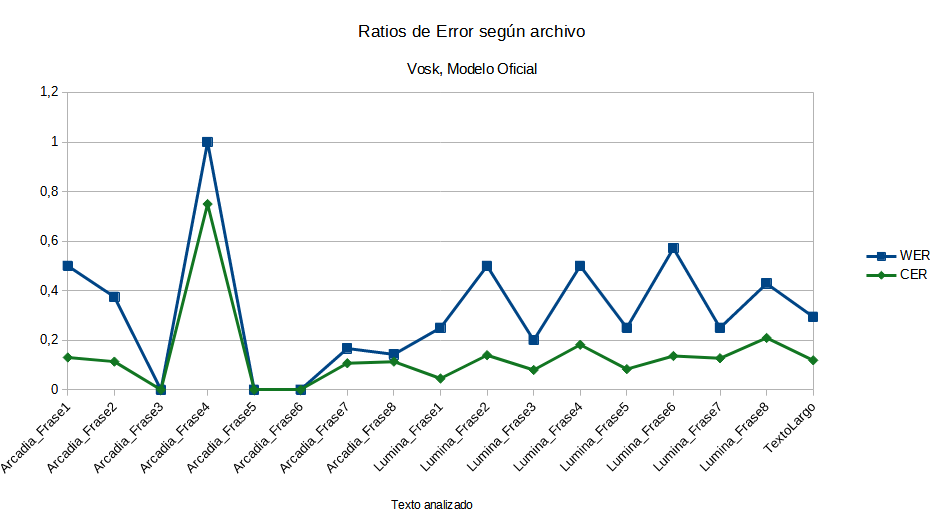
\includegraphics[width=\textwidth]{imagenes/WERCER_VoskIvan.png}
	\caption[Diagramas de WER y CER - Vosk]{Diagrama de los resultados al usar VOSK con el modelo que ofrecen en la web. Elaboración propia.}
\end{figure}

\begin{table}
\begin{tabularx}{\textwidth}{|c|X|}
	\hline
	Texto & Predicción \\ \hline
	 Frase 1 (Arcadia) & arabia entiende la luz \\ \hline
	 Frase 1 (Lúmina) & lubina enciende la luz  \\ \hline
	 Frase 2 (Arcadia)& arcadia pone esa canción y tanto me gusto \\ \hline
	 Frase 2 (Lúmina)& nómina por mí esa canción que tanto me gustó \\ \hline
	 Frase 3 (Arcadia)& arcadia repite lo que diga \\ \hline
	 Frase 3 (Lúmina)& nómina repite lo que diga \\ \hline
	 Frase 4 (Arcadia)& porque había para \\ \hline
	 Frase 4 (Lúmina)& nómina para \\ \hline
	 Frase 5 (Arcadia)& arcadia espera un momento \\ \hline
	 Frase 5 (Lúmina)& nómina espera un momento \\ \hline
	 Frase 6 (Arcadia)& arcadia reproduce el informativo de la mañana \\ \hline
	 Frase 6 (Lúmina)& nómina reproducen informativos de la mañana \\ \hline
	 Frase 7 (Arcadia)& marcaría con una alarma a las ocho y media de la mañana \\ \hline
	 Frase 7 (Lúmina)& lubina con una norma a las ocho y media de la mañana \\ \hline
	 Frase 8 (Arcadia)& arcadia prepara un temporizador de cinco minutos \\ \hline
	 Frase 8 (Lúmina)& nómina preparado un temporizador de cinco minutos \\ \hline

\end{tabularx}
\caption{Transcripciones de Vosk para las frases analizadas.}
\end{table}

En el caso de Vosk, se aprecia que el Ratio de Error de Palabra es bastante difuso en las Frases cuando se usa Arcadia como \textit{trigger word} (de hecho, en una de las frases no ha acertado ni una palabra). Cuando vemos las frases donde se usa Lúmina como trigger word, el ratio es más alto pero menos difuso, encontrándose entre el 20 y casi el 60\%. En cuanto al texto más largo, ha captado una muy buena parte del mensaje. 
Si se tiene en cuenta que es un modelo de 55 MB una vez descomprimido, ofrece resultados bastante completos.

\newpage

\subsubsection{DeepSpeech con Modelo Rhasspy y Scorer Poco}

\begin{figure}[H]
	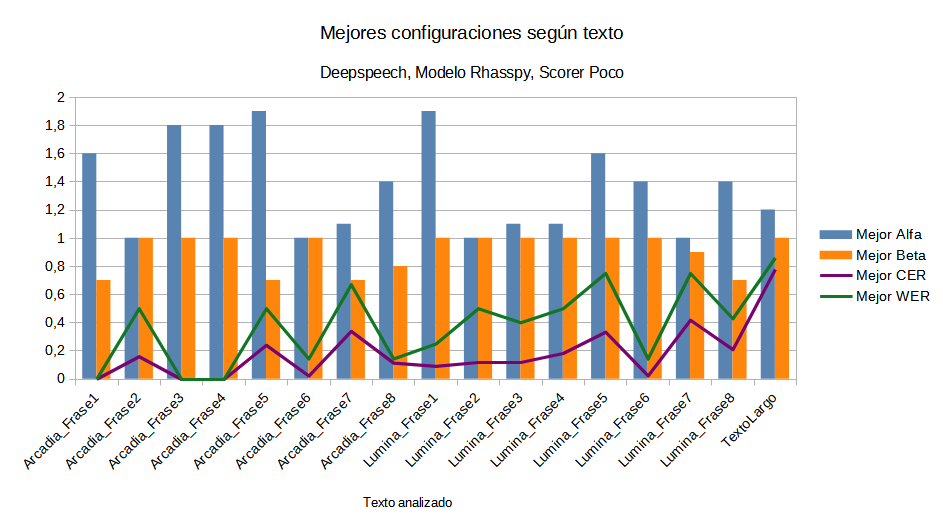
\includegraphics[width=\textwidth]{imagenes/MejoresResultados_DeepSpeechIvanPocoRhasspy.png} \\
	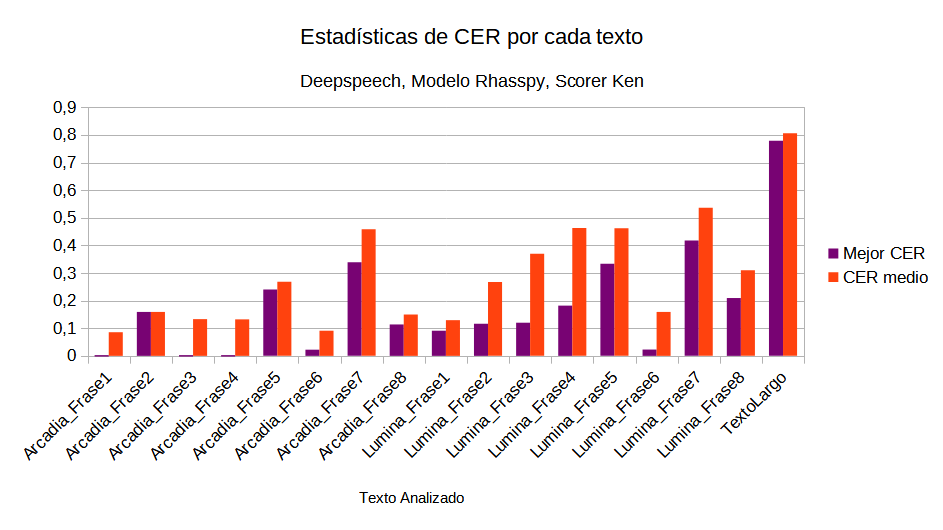
\includegraphics[width=0.5\textwidth]{imagenes/CER_DeepSpeechIvanPocoRhasspy.png} \hfill 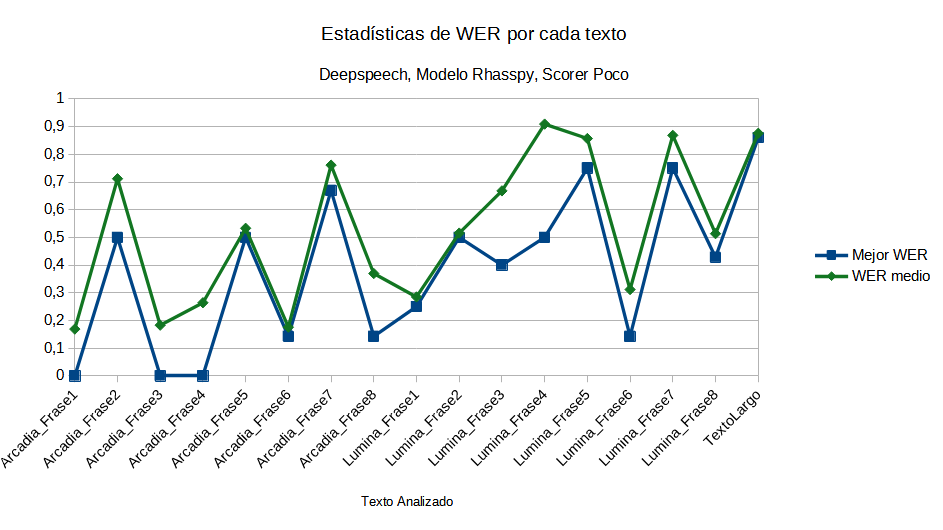
\includegraphics[width=0.5\textwidth]{imagenes/WER_DeepspeechIvanPocoRhasspy.png}
	\caption[Diagramas de Alfa, Beta, WER y CER - Rhasspy y Ken]{Diagrama de los resultados al usar Deepspeech con el modelo Rhasspy y el scorer Poco. Elaboración propia.}
\end{figure}

Empezando en las combinaciones con DeepSpeech, donde se usa el Modelo Rhasspy y el Scorer más completo, podemos ver que los valores más óptimos de Beta se encuentran entre el 0.7 y el 1, pero los valores de Alfa son más dispares. 

Podemos apreciar también que la mayor disparidad entre lo que la red neuronal predice y lo que realmente se quería decir es del 85\% en el texto más largo. Las frases que comienzan en Arcadia parecen reconocerlas mejor que las que comienzan por Lúmina.

\subsubsection{DeepSpeech con Modelo Rhasspy y Scorer Ken}

\begin{figure}[H]
	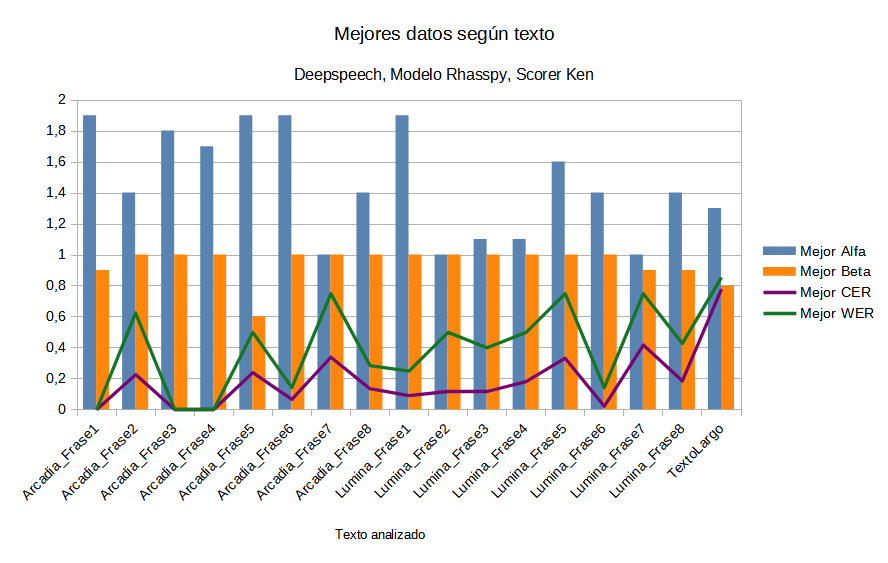
\includegraphics[width=\textwidth]{imagenes/MejoresResultados_DeepSpeechIvanKenRhasspy.png} \\
	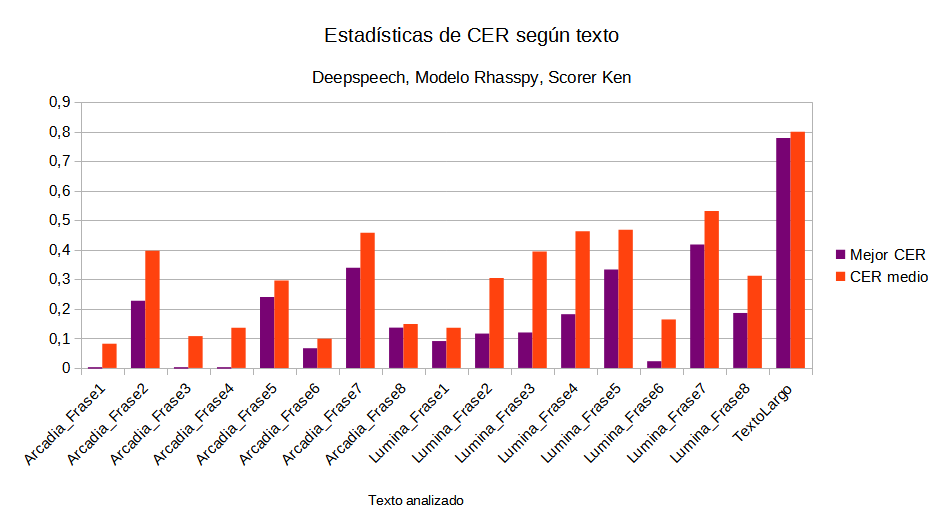
\includegraphics[width=0.5\textwidth]{imagenes/CER_DeepSpeechIvanKenRhasspy.png} \hfill 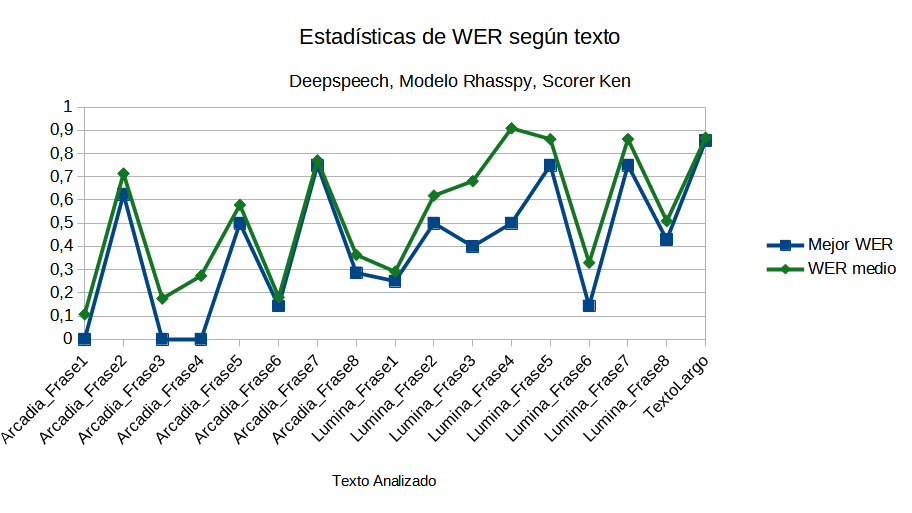
\includegraphics[width=0.5\textwidth]{imagenes/WER_DeepspeechIvanKenRhasspy.png}
	\caption[Diagramas de Alfa, Beta, WER y CER - Rhasspy y Ken]{Diagrama de los resultados al usar Deepspeech con el modelo Rhasspy y el scorer Ken. Elaboración propia.}
\end{figure}

En esta combinación se usa el Modelo Rhasspy y el Scorer Ken, y podemos ver que los valores más óptimos de Beta se encuentran casi siempre en el 1, pero los valores de Alfa son bastante altos cuando se trata de reconocer una frase llamando a la primera opción como trigger word, generalmente entre 1,7 y 1,9. En cuanto a la segunda opción, los resultados o están muy bajos (cerca del 1,1) o altos (1,4 al 1,6 salvo la primera frase que usa un valor de 1,9).

La tónica se repite con esta combinación,donde el ratio de error en el texto largo es altísimo y reconoce muy bien el nombre de Arcadia frente al de Lúmina. En cuanto al ratio de error a nivel de caracteres, podemos ver que es muy similar al anterior.

\subsubsection{DeepSpeech con Modelo Polyglot y Scorer Poco}

\begin{figure}[H]
	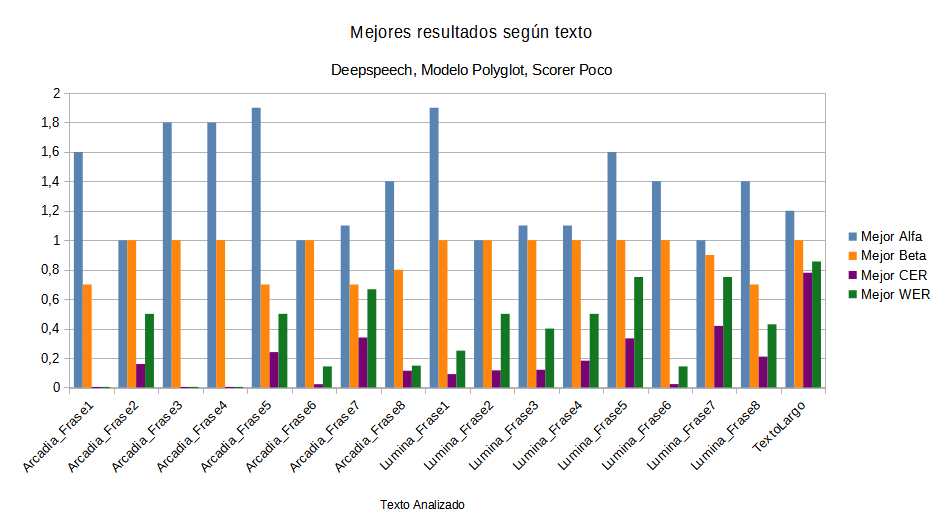
\includegraphics[width=\textwidth]{imagenes/MejoresResultados_DeepSpeechIvanPocoPolyglot.png} \\
	\includegraphics[width=0.5\textwidth]{imagenes/CER_DeepSpeechIvanPocoPolyglot.png} \hfill 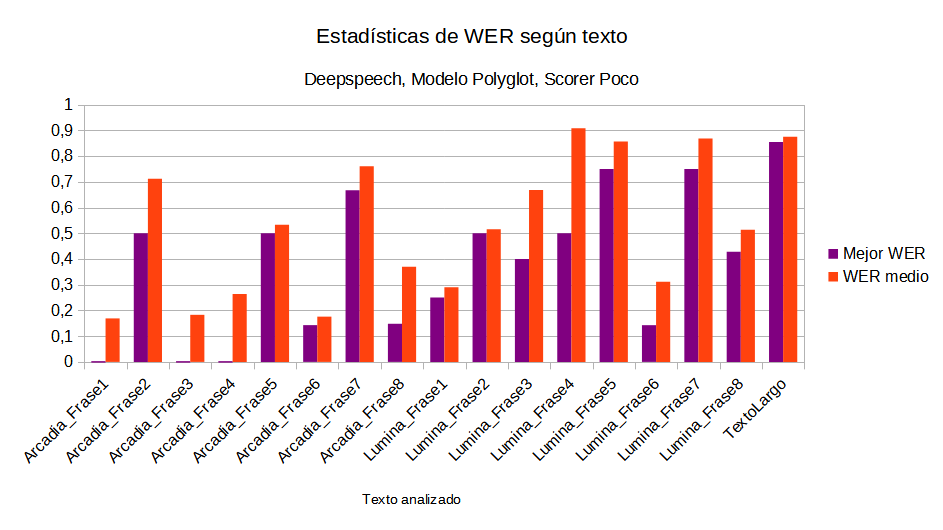
\includegraphics[width=0.5\textwidth]{imagenes/WER_DeepspeechIvanPocoPolyglot.png}
	\caption[Diagramas de Alfa, Beta, WER y CER - Polyglot y Poco]{Diagrama de los resultados al usar Deepspeech con el modelo Polyglot y el scorer Poco. Elaboración propia.}
\end{figure}

En este caso se usa el modelo Polyglot con el Scorer Poco. Los valores de Beta casi siempre están a 1, o al menos más allá de 0,7. En cuanto al Alfa, hay una tendencia a valores más altos en el caso de Arcadia, y a valores más bajos en el caso de Lúmina.

El valor del WER y del CER es muy parecido a los dos anteriores. Se sigue manteniendo la tendencia de que los textos largos tienen un valor alto. De hecho, si vemos esa opción, observamos que reconoce unos cuantos segundos y encima con muchos errores.

\subsubsection{DeepSpeech con Modelo Polyglot y Scorer Ken}

\begin{figure}[H]
	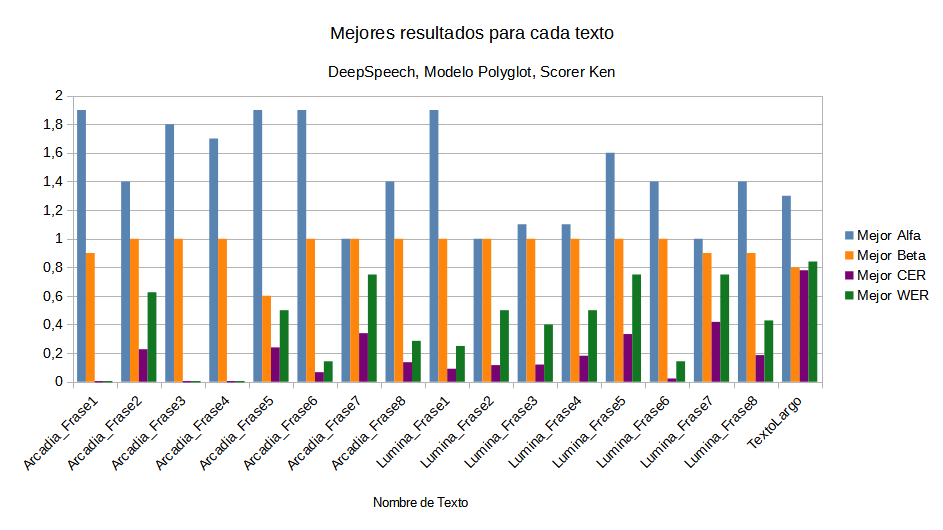
\includegraphics[width=\textwidth]{imagenes/MejoresResultados_DeepSpeechIvanKenPolyglot.png} \\
	\includegraphics[width=0.5\textwidth]{imagenes/CER_DeepSpeechIvanKenPolyglot.png} \hfill 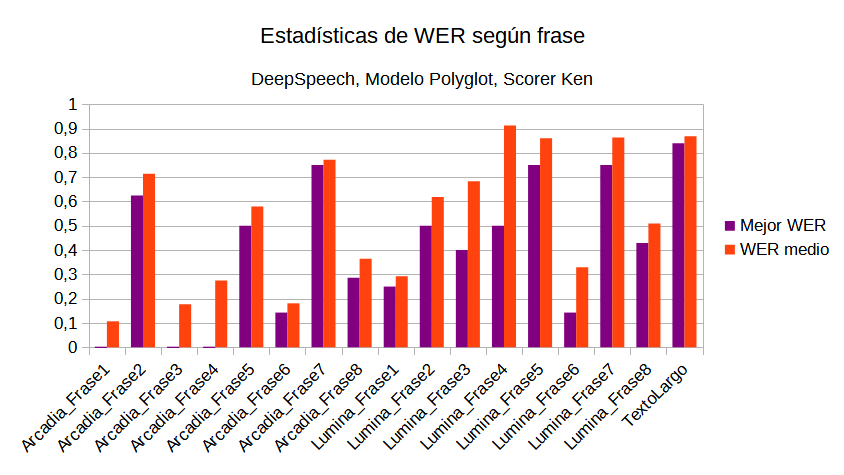
\includegraphics[width=0.5\textwidth]{imagenes/WER_DeepspeechIvanKenPolyglot.png}
	\caption[Diagramas de Alfa, Beta, WER y CER - Polyglot y Ken]{Diagramas de los resultados al usar Deepspeech con el modelo Polyglot y el scorer Ken. Elaboración propia.}
\end{figure}

En la combinación del modelo Polyglot con el Scorer más liviano, los valores de Beta casi siempre están a 1, es decir, viene mejor cuanta más penalización se da por fallar. En cuanto al Alfa, hay una tendencia a valores más altos en el caso de Arcadia, y a valores más bajos en el caso de Lúmina, como en la anterior ocasión.

El valor del WER y del CER es muy parecido a los dos anteriores. Se sigue manteniendo la tendencia de que los textos largos tienen un valor alto, algo que vemos constante en los experimentos con DeepSpeech. De hecho, podemos ver en comparación lo que han deducido las 4 combinaciones de DeepSpeech y la otra API (véase tabla \ref{tab:predicts} en la página \pageref{tab:predicts})

\begin{table}
	\begin{tabularx}{\textwidth}{|c|X|}
		\hline
		\makecell{Vosk} & lo la y arcadia se encuentran en un portal a medio camino entre sus casas cerca del centro comercial ellas habían quedado para ver la nueva película que tanto proporcionaban por la tele y buscar un momento entre su agenda para ir a verla comparte un beso auriculares con su amiga y entienden entre spotify y reproduce el tema de que perdí mientras pasión hacia su destino al llegar buscar el cine y la entrada de las palomitas para la sala un temporizador de cinco minutos en la pantalla que además no paraba de poner publicidad de repente todo separa por un corte de luz toda esta oscura si alguien entiende la luz de su teléfono aunque no sirve de mucho hasta que vuelva suministro funcionar y ya puedan ver la película al terminar ya que tiempo hace para saber si esperar a que recojan o volver andando aunque lo piensa mejor tras mirar qué hora es y venir tomar un café antes de irse \\ \hline
		\makecell{DeepSpeech,\\ Modelo Rhasspy,\\ Scorer Poco} & una arcadia se encuentran en un portal a medio camino entre sus casas cerca del centro comercial ella habian quedado para ver la nueva pelicula que tanto proporcionada por la tele y buscar numenoreanos eeaaoaeecaoeee \\ \hline
		\makecell{DeepSpeech,\\ Modelo Rhasspy,\\ Scorer Ken} & una arcadia se encuentran en un portal a medio camino entre sus casas cerca del centro comercial ella habian quedado para ver la nueva pelicula que tanto proporcionada por la tele y buscar numenoreanos eeaaoaeecaoeee \\ \hline
		\makecell{DeepSpeech,\\ Modelo Polyglot,\\ Scorer Poco} & una arcadia se encuentran en un portal a medio camino entre sus casas cerca del centro comercial ella habian quedado para ver la nueva pelicula que tanto proporcionada por la tele y buscar numenoreanos eeaaoaeecaoeee \\ \hline
		\makecell{DeepSpeech,\\ Modelo Polyglot,\\ Scorer Ken} & una arcadia se encuentran en un portal a medio camino entre sus casas cerca del centro comercial ella habian quedado para ver la nueva pelicula que tanto proporcionada por la tele y buscar numenoreanos eeaaoaeecaoeee\\ \hline
		
	\end{tabularx}
	\caption{Textos que arrojan las APIs al analizar el audio más largo.}
	\label{tab:predicts}
\end{table}

\subsection{Conclusiones}

Si bien hemos hablado de los datos en su propio contexto, ¿qué pasa si comparamos los resultados entre sí? Para poder sacar conclusiones, se ha exportado las respuestas finales en gráficas para comparar su rendimiento ante las mismas pruebas.

\begin{figure}[H]
	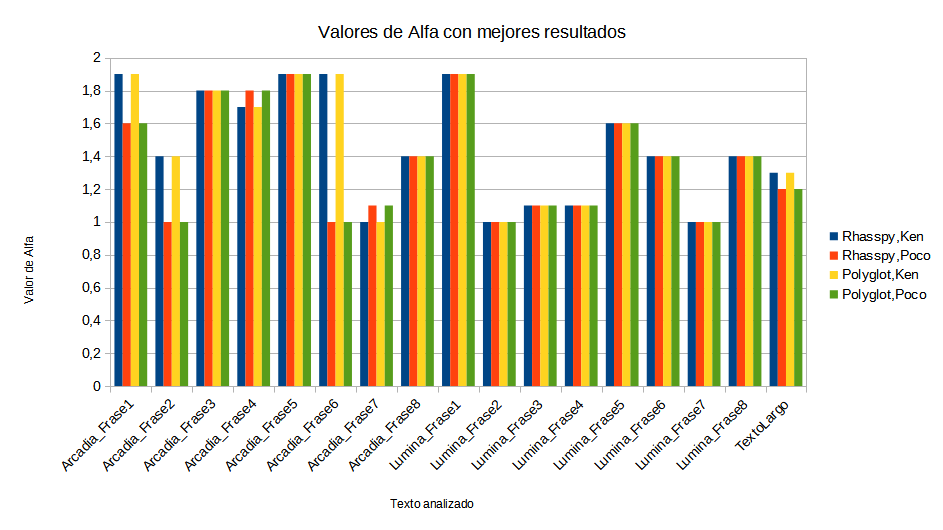
\includegraphics[width=0.9\textwidth]{imagenes/Alfas.png} \hfill 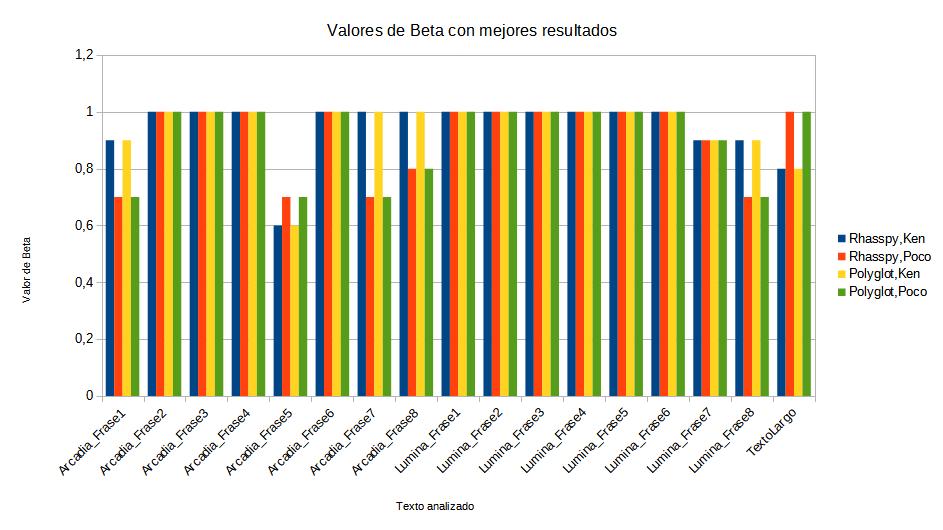
\includegraphics[width=0.9\textwidth]{imagenes/Betas.png}
	\caption{Gráficas comparativas de los valores de Alfa y Beta con los mejores resultados, según la frase y la combinación de Modelo y Scorer. Elaboración propia}
\end{figure}

En el caso de DeepSpeech, los ajustes de Alfa y Beta son iguales en el caso de los modelos, por lo que usar uno u otro no nos daría ninguna ventaja. Por otro lado, los scorers sí alteran los parámetros, observando que en el Scorer Poco se da el mismo o menos peso al modelo del lenguaje en general que en Scorer Ken (como excepción podemos ver en la Frase 7 con Arcadia que el peso es menor). También se le da menos castigo en el predictor más completo (salvo en el Texto Largo y la Variante con Arcadia de la Frase 5).

\begin{figure}[H]
	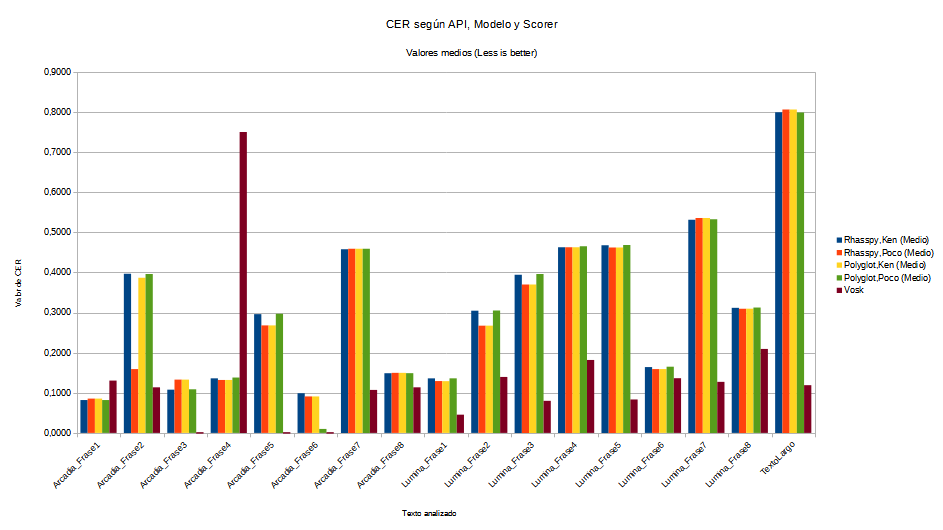
\includegraphics[width=\textwidth]{imagenes/CERMedios.png} \hfill 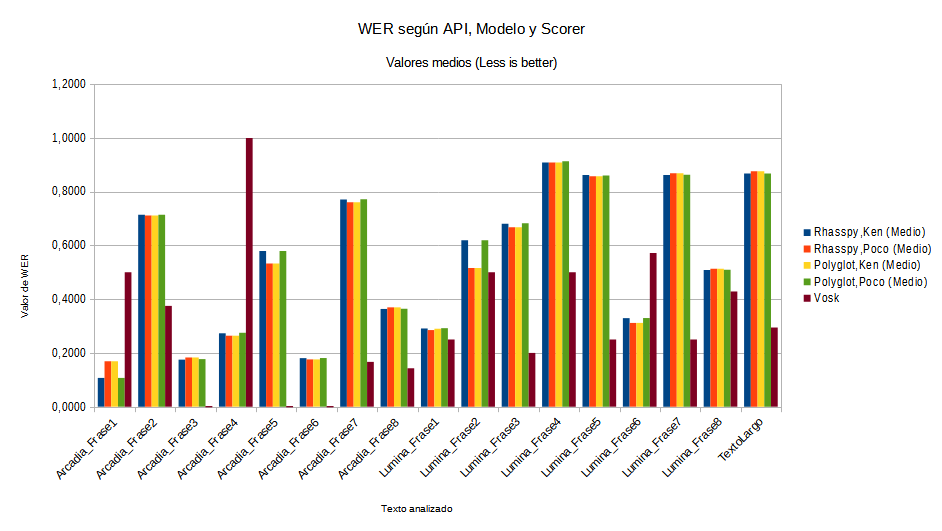
\includegraphics[width=\textwidth]{imagenes/WERMedios.png}
	\caption{Gráficas comparativas de los valores medios de WER y CER, según la frase y la combinación de Sistema, Modelo y Scorer (donde proceda). Elaboración propia}
\end{figure}

Por el Character Error Rate, vemos que al comparar letra a letra Vosk mantiene unos niveles bastante bajos salvo por su pico del 75\%. En cuanto al Ratio de Error a nivel de palabra, la cifra sube a valores de hasta un 50\% salvo en la misma frase del pico anterior, donde falla toda la predicción.
En el caso de DeepSpeech, hay muy pocas diferencias en sus valores medios entre sus 4 variantes. Como hemos visto anteriormente, debido a su comportamiento en el texto largo donde reconoce unos cuantos segundos, las relaciones de errores se disparan al tope del 80
\% en el caso del CER y del casi 90\% en el caso del WER

\begin{figure}[H]
	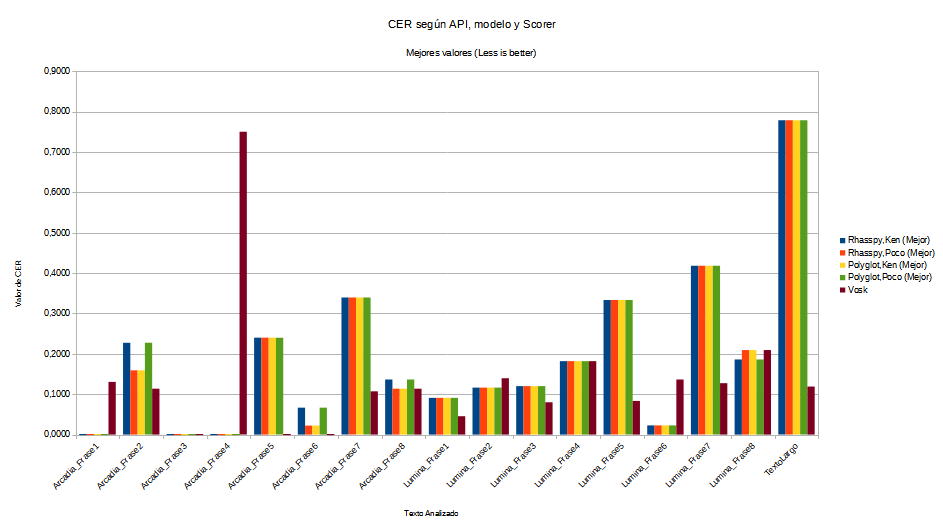
\includegraphics[width=0.9\textwidth]{imagenes/CERMejores.png} \hfill 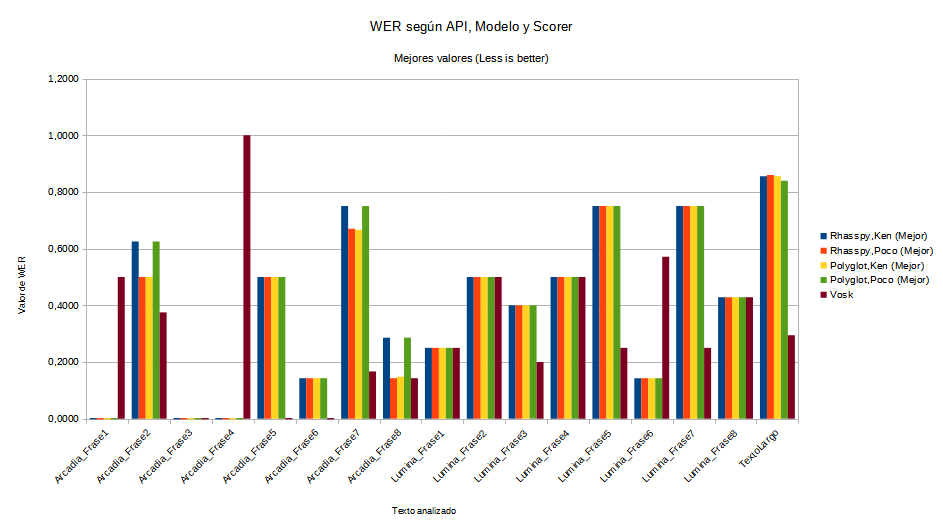
\includegraphics[width=0.9\textwidth]{imagenes/WERMejores.png}
	\caption{Gráficas comparativas de los mejores valores de WER y CER, según la frase y la combinación de Sistema, Modelo y Scorer (donde proceda). Elaboración propia}
\end{figure}

En cuanto a los resultados arrojados en las mejores generaciones, vemos que en el frente de DeepSpeech sigue siendo bastante homogéneo, si bien la combinación del Modelo Polyglot con el Scorer Ken es algo mejor en algunas ocasiones. Sin embargo, hay muchos casos donde Vosk es mejor que las 4 combinaciones, aunque podemos ver puntos aislados sorprendentes, como ver que DeepSpeech ha sido capaz de descifrar perfectamente qué se estaba hablando, cuando la alternativa falló completamente.

Otra conclusión que podemos sacar son, por ejemplo, que de los nombres propuestos, ``Arcadia'' se reconoce más veces que ``Lúmina'' (de hecho, esta última se ha reconocido sólo una vez por DeepSpeech), aunque a veces se confundan con otras palabras (como \textit{arabia}, \textit{marcaría}, o \textit{nómina}). Para permitir que se entendieran perfectamente estas palabras habría que entrenar los modelos para que las aceptaran e integraran en su vocabulario. Eso sí, hacerlo requeriría varias tarjetas gráficas y un tiempo de procesamiento de alrededor de 100 horas para hacer una sintonía fina. Otra opción sería poner alguna palabra parecida como \textit{trigger word} también, pero eso haría activarse el asistente en alguna ocasión inesperada según si la palabra es más o menos común. 

Por lo visto sobre los nombres, en este estado podemos darle nombre a nuestro Asistente en función del comportamiento de las opciones cuando se menciona esta palabra. También en este punto podemos elegir la API que menos fallo nos daría. Para ello, vamos a comprobar su promedio y desviación típica.

\begin{xltabular}{\textwidth}{|X|X|X|X|X|}
	\hline
	Método & CER Promedio & Desv. Típica de CER & WER Promedio & Desv. Típica de WER \\ \hline
	DeepSpeech + Rhasspy + Ken (\textbf{Mín.}/Medio) & \textbf{0,1916}/0,3115 & \textbf{0,1968}/0,1966 & \textbf{0,4047}/0,5349 & \textbf{0,2855}/0,2763 \\ \hline
	DeepSpeech + Rhasspy + Poco (\textbf{Mín.}/Medio) & \textbf{0,1850}/0,2929 & \textbf{0,1993}/0,1990 & \textbf{0,3845}/0,5277 & \textbf{0,2814}/0,2705 \\ \hline
	DeepSpeech + Polyglot + Ken (\textbf{Mín.}/Medio) & \textbf{0,1850}/0,3063 & \textbf{0,1993}/0,1971 & \textbf{0,3844}/0,5280 & \textbf{0,2805}/0,2702 \\ \hline
	DeepSpeech + Polyglot + Poco (\textbf{Mín.}/Medio) & \textbf{0,1916}/0,3070 & \textbf{0,1968}/0,2038 & \textbf{0,4038}/0,5357 & \textbf{0,2840}/0,2763 \\ \hline
	Vosk & \textbf{0,1375} & \textbf{0,1689} & \textbf{0,3194} & \textbf{0,2537} \\ \hline
\end{xltabular} 

Por los datos arrojados, la API que más nos convendría usar es Vosk, ya que tiende a acertar más lo que se quiere decir. 

También tenemos un nombre para nuestro asistente, pudiendo añadir algo de personalidad al producto resultante, siendo este \textit{Arcadia}.

\section{Eligiendo una API de Síntesis de Voz}
Por la otra parte, sintetizar la voz nos permite ofrecer el feedback al usuario los resultados a lo que se piden. Al igual que en el Reconocimiento del Habla, las grandes compañías tienen su propia implementación en un formato "Software como servicio" (como Google TTS o IBM Watson TTS).

En este campo tenemos también otro par de APIs que usan sistemas de Código Abierto. Estos son:

\begin{itemize}
	\item \textbf{Festival TTS} \cite{festival}: Creada por la Universidad de Edimburgo, usa una licencia del tipo X11/MIT. Se ofrece como un framework general para la síntesis de voz a través de varias APIs, ofreciendo así que se pueda usar embebido en un programa escrito en Java, dentro del propio shell o como librería de C++ (y a través de una interfaz, se puede usar con Python).
	\item \textbf{eSpeakNG} \cite{espeak} \cite{espeak-ng}: Creado por Jonathan Duddington, se trata de un sintetizador de voz que usa el método de síntesis formante, permitiendo que las voces se representen con modelos muy ligeros, pero cuyos resultados no son muy naturales. Se licencia con GPL versión 3 \cite{gplv3}.
	Como nota aparte, se puede combinar con el sintetizador MBROLA para mejorar la voz, pero estas voces mejoradas poseen una cláusula modificada por la cual exigen que no se puede ganar beneficios con ellas en sí o embebidas en un software mayor.
	 \item \textbf{NanoTTS} \cite{nanotts}: Es una reimplementación de SVOX Pico TTS, usado en la versión Open Source de Android, de la que coge las voces y la parte libre de Pico para formar un programa propio. Emplea una licencia Apache 2.0, al igual que las voces y la parte abierta.
\end{itemize}

En este ámbito, no se puede elegir el mejor programa en base a temas objetivos, sino que va más al gusto del usuario. Para ello, se ha valorado por una parte la facilidad de uso de la API, y por la otra, cómo de humana suena esa voz (de forma subjetiva).

Por la parte de facilidad de uso, he usado paquetes complementarios de pip para unir el programa con Python y así poder generar las frases desde el sistema. En ese sentido, la facilidad de uso ha sido bastante similar en el caso de \textbf{eSpeakNG} y \textbf{Festival}, ya que estas APIs requerían el uso de una librería de tratamiento de archivos .wav para hacer una copia a un archivo que tuviéramos a mano. En el caso de \textbf{NanoTTS} ha sido mucho más sencillo ya que su wrapper para Python tiene un constructor donde puedes poner cómo se llama el archivo. 

Además, en el caso del wrapper de \textbf{Festival}, hablamos de un paquete obsoleto que no deja cambiar la voz a una versión española, lo que supone un riesgo, ya que habría que parchear el código del paquete para poder cambiar la voz y otros parámetros, ya que parece estar desatendido. Por lo tanto, descartaría la opción de Festival entre los candidatos.

En cuanto a mi percepción personal sobre cómo suenan las otras dos voces:
\begin{itemize}
	\item En el caso de \textbf{eSpeak}, no se nota muy robótica y además se puede personalizar bastante, pero hay algo en el producto generado que falla, y es que sale una especie de fonema extraño que suena en cada palabra, lo que puede ser algo molesto.
	\item Sobre \textbf{NanoTTS}, me ha parecido una voz más realista con ajustes bastante similares a los del anterior, siendo su pega más relevante unas pausas quizás un poco más largas de lo normal.
\end{itemize}

En conclusión, usaré NanoTTS para que Arcadia nos hable. Pero ahora que nos puede hablar y escuchar, sólo nos quedaría conectar ambas partes.

\section{Relacionando preguntas y respuestas.}
Una vez que podamos pasar a texto las preguntas y que además el texto que respondamos se pueda convertir a voz, falta dotar a nuestro Asistente con algo de funcionalidad y una base de conocimientos para que nos pueda decir algo coherente.

En este caso, nos encontramos con algunas alternativas que responden a distintos tipos de funcionamiento:

\begin{itemize}
	\item \textbf{Pattern-matching}
	Aquí nos podemos encontrar algunos casos como:
	\begin{itemize}
		\item \textbf{AIML} \cite{aiml} En el paso por la carrera los estudiantes están familiarizados con este lenguaje de marcado anteriormente, en la asignatura de Inteligencia Artificial. Si bien permitía hacer cierta funcionalidad, no puede usar peticiones de APIs para poder completar información en sus últimas versiones, por lo que queda descartada. Además, su sintaxis puede llegar a ser compleja de entender, ya que se necesita una estructura con muchas etiquetas para funciones más dificultosas.
		\item \textbf{RiveScript} \cite{rivescript} Es una versión de AIML más simplificada y clara, pero tiene mucha de su funcionalidad, aparte de algunas funciones extra (como más condicionales o temas que puedan ser heredados de otros temas de conversación). Sin embargo, hacer un embed de Python con un cliente de RiveScript conllevaría un tiempo considerable.
		\item \textbf{ChatScript} \cite{chatscript} En este caso hablamos de un lenguaje de script superior a los anteriores, pero cae en el mismo problema que RiveScript. Y es que su único cliente está desarrollado en C, si bien se podría adaptar a Python gracias a la librería que tiene para invocar funciones de C.
	\end{itemize}	
	\item \textbf{Procesamiento del lenguaje natural (NLP)}
	Si bien hay opciones propietarias como \textbf{\underline{DialogFlow}} \cite{dialogflow}, al mirar opciones de Código Abierto costó dar con uno, pero finalmente apareció la opción de usar \textbf{\underline{Rasa}} \cite{rasa}, que aunque no tenía mucha documentación en español, era bastante completa y esmerada, y con bastantes vídeos y tutoriales que me ayudaron a entender cómo usarlo.
\end{itemize}

Al comparar ChatScript y Rasa para decidir cuál usar, se ha observado que el hecho de que Rasa esté en continuo desarrollo, la flexibilidad de sus modelos y la facilidad para entrenarlos me ha servido de punto de inflexión para elgir esta herramienta frente a la opción por patrones.
	
\section{Diseñando el problema}

En resumen hasta ahora, hemos conseguido los tres grandes ingredientes que componen a nuestro proyecto. Ahora que los tenemos, ya nos queda preparar el problema y sus diagramas para facilitar el desarrollo.

\subsection{Diagrama de casos de uso}
En este proyecto, los casos de uso en general tienen sólo un actor humano, que sería el usuario que interactúa con el software. Pero también hemos de incluir un actor que intervendría en el desarrollo, que en este caso sería el chatbot, ya que si bien se desarrolla, al final interactúa con el software y sería capaz de funcionar independientemente.

El flujo básico de Arcadia estaría definido por el siguiente diagrama de casos de uso, donde ambos actores interactúan en el transcurso entre que el usuario diga una petición y el mismo reciba la respuesta.

\begin{figure}[H]
	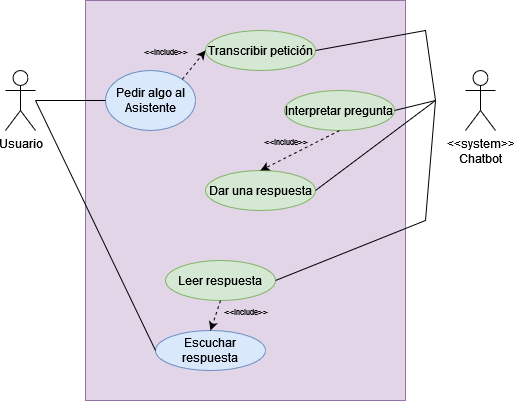
\includegraphics[width=0.75\textwidth]{imagenes/DiagramaCasosUso.png}
	\caption{Diagrama de casos de uso. Elaboración propia.}
\end{figure}

\subsection{Diagrama de clases}
\subsubsection{Grabación y streaming de audio}
Para la grabación del audio podemos usar FFmpeg \cite{ffmpeg} o PyAudio \cite{pyaudio} indistintamente, ya que ambos sistemas de codificación del audio son bastante capaces para esta tarea. Esto implicaría hacer uso del patrón Adaptador para crear una abstracción entre los métodos o ejecuciones del software existente y nuestro sistema para cada opción.
En este caso podríamos seguir esta manera de construir software para tener varias versiones de esa funcionalidad con sistemas distintos. (Aunque en la práctica lo más probable es que lo haga con uno de ellos, pero gracias a ello podemos darle modularidad al sistema para cambiarlo en cualquier momento).

\begin{figure}[H]
	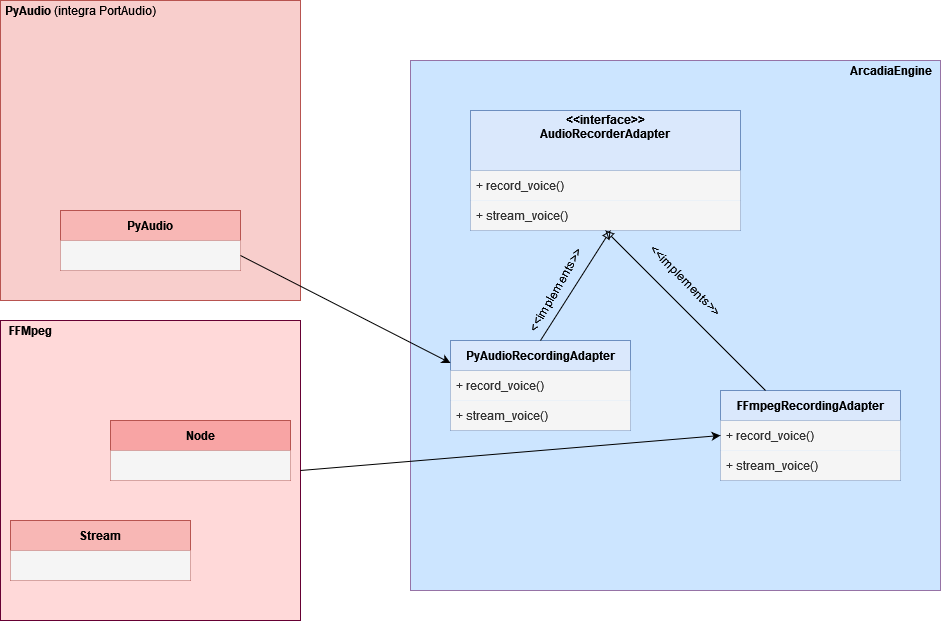
\includegraphics[width=\textwidth]{imagenes/DiagramaClases_Grabacion.png}
	\caption{Diagrama de clases relacionadas con la grabación del sonido. Elaboración propia.}
\end{figure}

\subsubsection{Reconocimiento de voz}
Para el reconocimiento de voz se hará uso de una clase que sirva de interfaz a las APIs que lo requieran, las cuales tendrán para poder usarse en el resto de la implementación una clase que sirva de adaptador. De esta manera, si quisiéramos usar otra API, sólo tendríamos que implementar los métodos del adaptador.
\begin{figure}[H]
	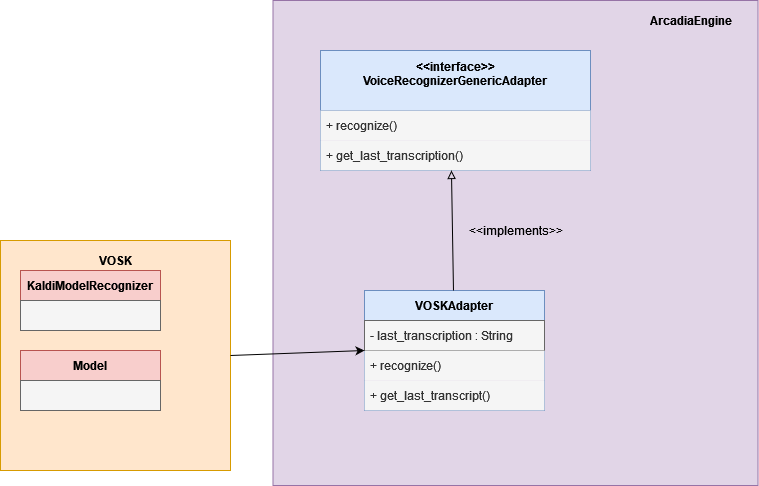
\includegraphics[width=\textwidth]{imagenes/DiagramaClases_SR.png}
	\caption{Diagrama de clases relacionadas con el Reconocimiento del habla. Elaboración propia.}
\end{figure}
\subsubsection{Procesamiento de la petición y creación de una respuesta}
Para procesar la petición, usaremos un adaptador como antes. En nuestro caso, además, trataremos con peticiones HTTP a través de REST entre nuestra implementación y Rasa, ya que se aloja en un puerto de nuestro PC escuchando las peticiones.

En la parte de Rasa, según su documentación, para desarrollar funcionalidades más complejas, podemos implementar en su entorno, en un fichero Python, clases que heredan de Action. Al estar alojados en otro puerto donde se comunica principalmente con el puerto de Rasa, interactúan entre sí para dar la respuesta.

Aquí podemos ver un detalle de las clases y sus relaciones, en este sentido:
\begin{figure}[H]
	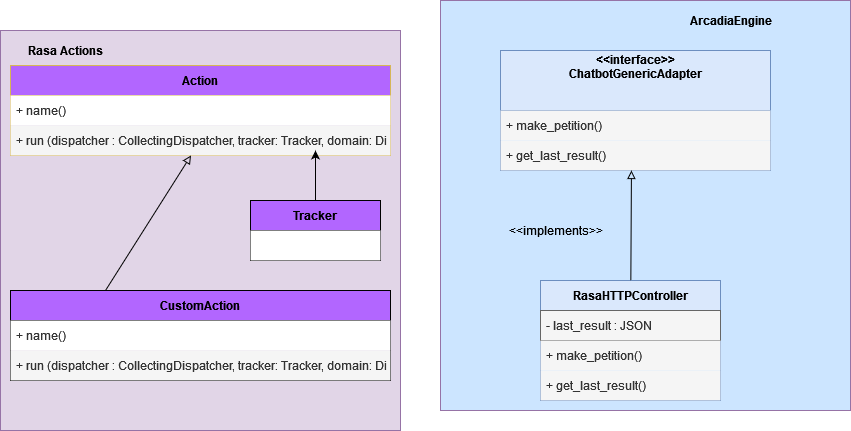
\includegraphics[width=\textwidth]{imagenes/DiagramaClases_Chatbot.png}
	\caption{Diagrama de clases relacionadas con la interacción con el Chatbot. Elaboración propia.}
\end{figure}
\subsubsection{Síntesis de voz}
De forma análoga al reconocimiento de voz, la síntesis precisará de un adaptador para facilitar el funcionamiento interno del asistente. De esta manera, lo conectaremos a NanoTTS para que nos convierta el texto a Voz.

\begin{figure}[H]
	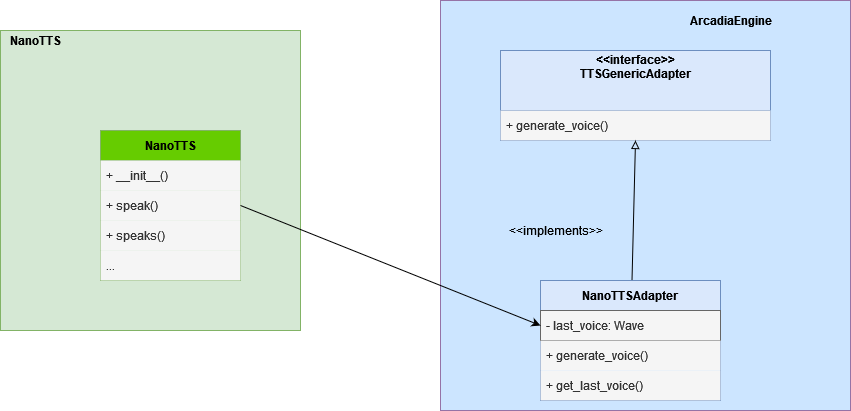
\includegraphics[width=\textwidth]{imagenes/DiagramaClases_TTS.png}
	\caption{Diagrama de clases relacionadas con la Síntesis de Voz. Elaboración propia.}
\end{figure}
\subsubsection{Reproducción de las respuestas}
Para la reproducción del audio podemos usar de nuevo FFmpeg o PyAudio indistintamente, ya que ambos sistemas pueden grabar y reproducir audio . Ya que esán importados, habría que hacer otros adaptadores sólo para el sentido de la reproducción.

\begin{figure}[H]
	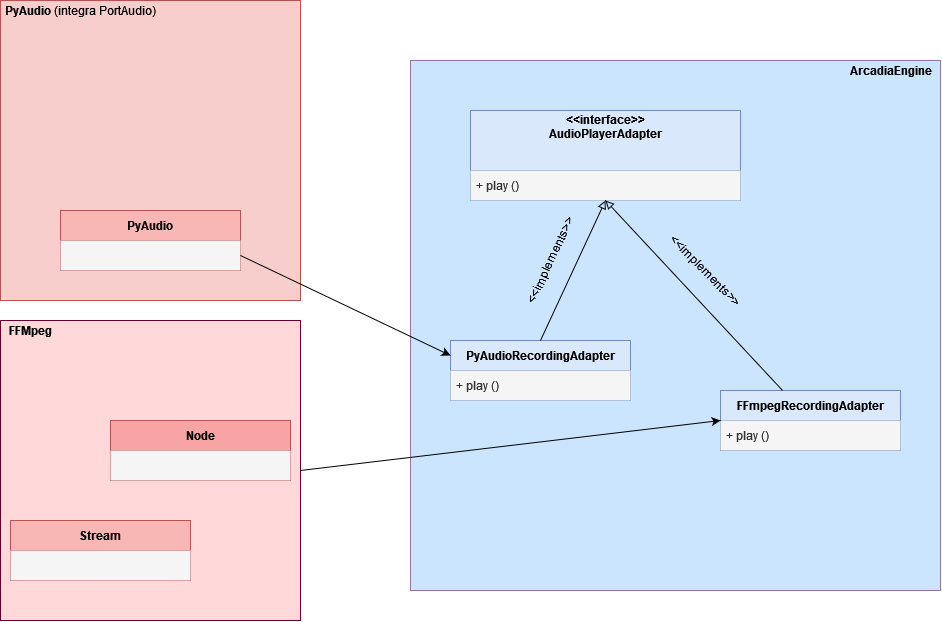
\includegraphics[width=\textwidth]{imagenes/DiagramaClases_Reproduccion.png}
	\caption{Diagrama de clases relacionadas con la reproducción del sonido. Elaboración propia.}
\end{figure}

El resultado final del diagrama de clases está en la página \pageref{fig:diagramaclases}, figura \ref{fig:diagramaclases} .
\begin{landscape}
	\begin{figure}
		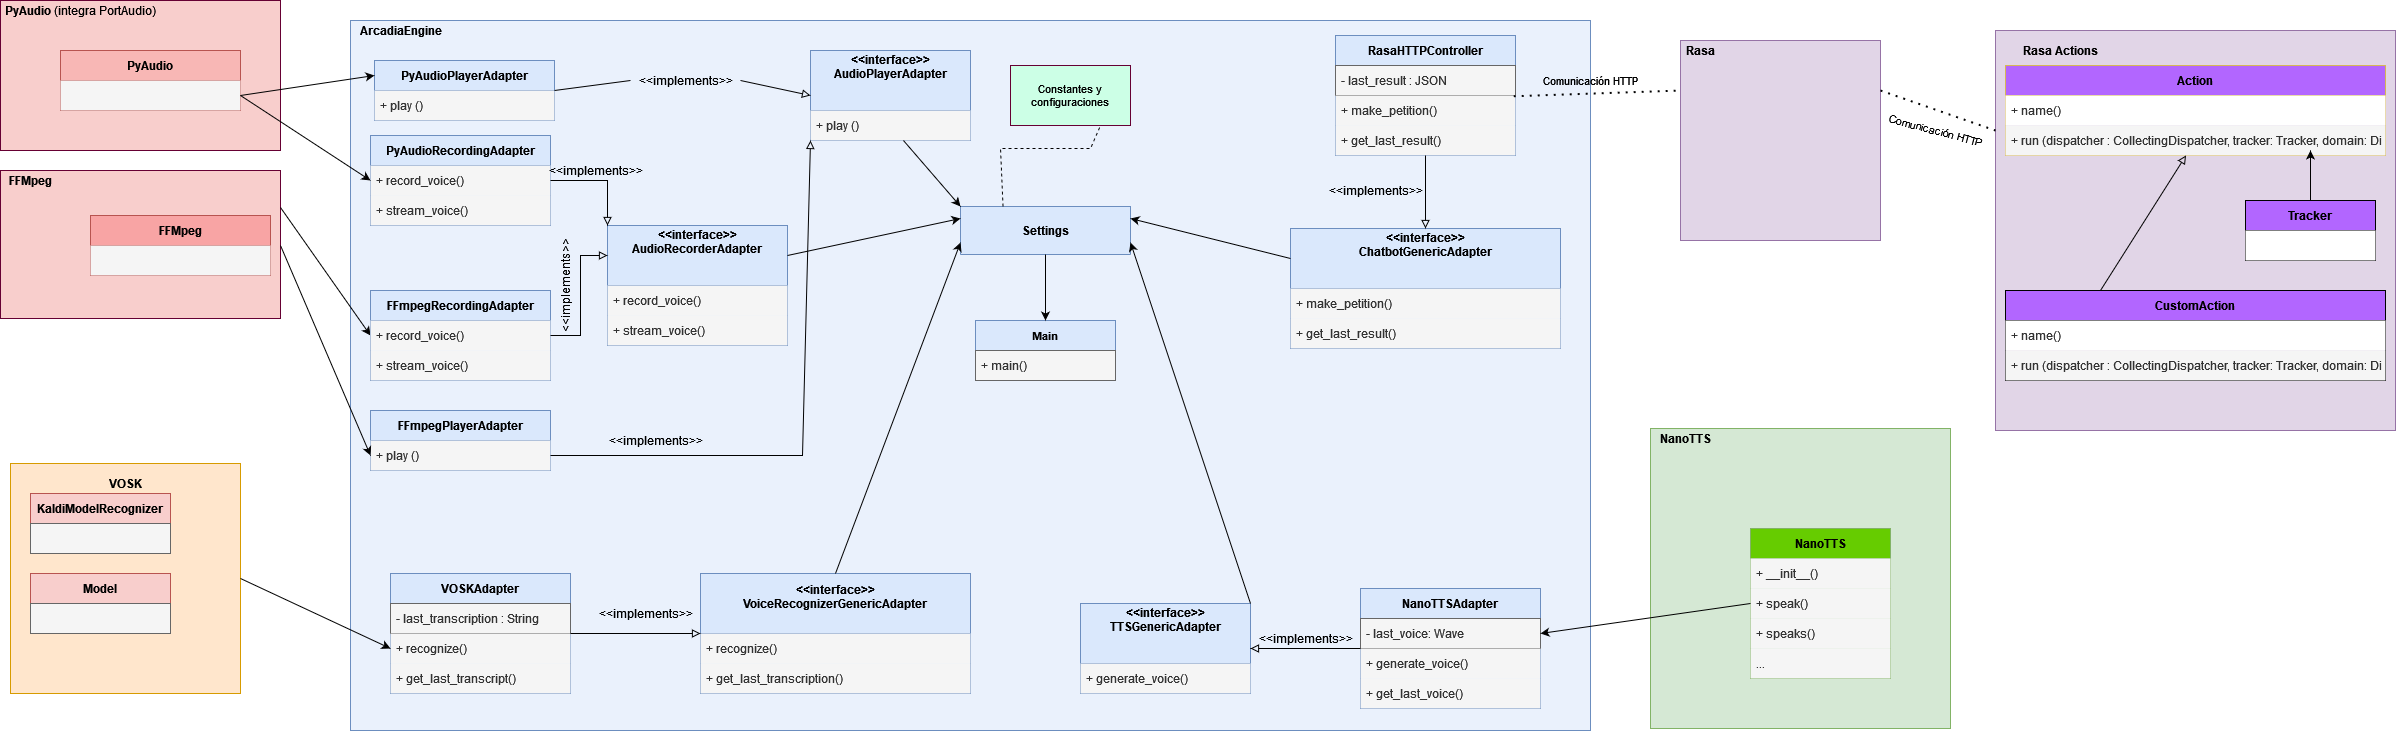
\includegraphics[width=1.5\textwidth]{imagenes/DiagramaClases_General.png}
		\caption{Diagrama de clases general.}
		\label{fig:diagramaclases}
	\end{figure}
\end{landscape}

\begin{table}[H]
	\centering
	\begin{tabularx}{\textwidth}{|>{\columncolor{mintgreen}}c>{\columncolor{mintgreen}}X|}
		\hline
		
\includegraphics[width=30pt]{imagenes/Tarea_completada.png} & Con ello, cumplimos los Objetivos \textbf{O-IA 4.} (Sintetizar los posibles componentes que conforman un Asistente de Voz y la escalabilidad de cada uno de ellos), \textbf{O-DD 2.} (Diseñar las clases que albergarán los componentes de un Asistente de Voz, su interacción con los periféricos de Entrada/Salida y con aquellas APIs externas que se requieran para el funcionamiento básico del programa) y \textbf{O-DD 3.} (Idear una vía para escalar el número de posibles frases e interacciones que pueda reconocer el proyecto) \\
		\hline
	\end{tabularx}
\end{table}

\subsection{Diagrama arquitectónico}
Por lo que vemos, nos encontramos con una arquitectura que dispone de programas externos que podemos usar en nuestro software gracias a sus respectivas APIs. Por nuestra parte, primero adaptamos toda su funcionalidad a nuestro ámbito en una serie de adaptadores para simplificar la información que luego llegará o saldrá de nuestro núcleo, que define el flujo básico del proyecto.

Por otra parte, tenemos una comunicación con Rasa, que a su vez tiene otra comunicación con Rasa Actions, para atender las peticiones más complejas. Desde Rasa Actions también se hará la gestión de consultas a algunas páginas de Internet.

\begin{center}
	\begin{figure}[H]
		\includegraphics[width=0.8\textwidth]{imagenes/DiagramaArquitectónico.png}
		\caption{Diagrama de la arquitectura de Arcadia. Elaboración propia.}
	\end{figure}
\end{center}

Por tanto, nos quedaríamos con la siguiente arquitectura, que parece derivado de una arquitectura en pizarra, pues poseemos varios agentes externos (Grabadores, Reproductores, TTS, Reconocedores y el Chatbot) que anotan o cogen en el programa principal la información (rutas de audios, transcripciones y resultados a peticiones). 

Además, cada parte del software tiene uno o dos objetivos en el sistema, lo que hace que sus funciones estén bien definidas y sepamos a dónde dirigirnos en caso de error.

Una diferencia de nuestra arquitectura con respecto a la idea general de una pizarra, sin embargo, viene por dos cuestiones:

\begin{itemize}
	\item La pizarra en sí está rodeada de clases adaptadoras para poder dar toda la información de forma más simple
	\item Hay dos fuentes de conocimiento que influyen en la arquitectura: las respuestas que nos ofrece el modelo en Rasa, y el estado del flujo principal en nuestra aplicación.
\end{itemize}


\begin{table}[H]
	\centering
	\begin{tabularx}{\textwidth}{|>{\columncolor{mintgreen}}c>{\columncolor{mintgreen}}X|}
		\hline
		
\includegraphics[width=30pt]{imagenes/Tarea_completada.png} & Con ello, cumplimos el Objetivo \textbf{O-DD 4.} (Planear la arquitectura del proyecto resultante, siguiendo las buenas prácticas del Desarrollo de Software) \\
		\hline
	\end{tabularx}
\end{table}


\subsection{Diagrama de flujo general}
 
 Una vez visto las piezas de este rompecabezas, toca ver el flujo que seguiría nuestro proyecto.
 
 Para ello, se ha representado en el diagrama todas sus funcionalidades de una forma más general.
 
 Para representarlo de forma más visual, y podamos ver qué acciones realiza cada elemento en su ámbito dentro del programa, se han coloreado las acciones según la parte que interviene en él:
 
 \begin{itemize}
 	\item En \textbf{\textcolor{red}{rojo}}, las acciones que requieran de controlar audios y grabaciones (como hemos dicho anteriormente, podemos usar librerías como PyAudio o FFMpeg)
 	\item En \textbf{\textcolor{yellow}{amarillo}}, aquellas de las que se encargue el Reconocedor de Habla (como Vosk)
 	\item En \textbf{\textcolor{violet}{violeta}}, las partes donde entra en juego el chatbot (Rasa), además de sus acciones vinculadas (en nuestro caso, Rasa Actions)
 	\item En \textbf{\textcolor{cyan}{azul}}, las acciones y decisiones que nuestra implementación debe controlar.
 \end{itemize}
 
 
 \begin{figure}[H]
 	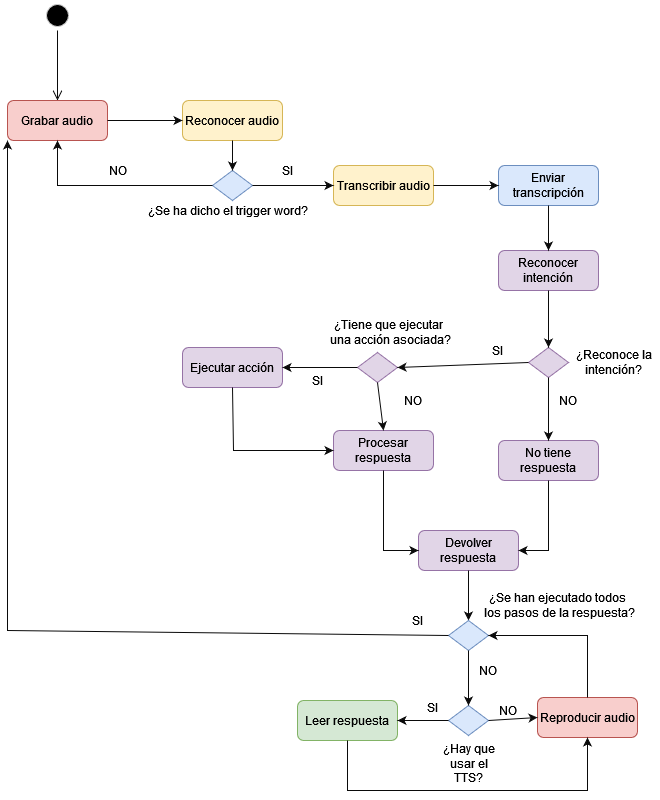
\includegraphics[width=\textwidth]{imagenes/DiagramaFlujo.png}
 	\caption{Diagrama del flujo general del sistema. Elaboración propia.}
 \end{figure}

 


	% Desarrollo bajo sprints: 
	% 	1. Permitir registros y login de usuarios
	% 	2. Desarrollo del sistema de incidencias
	% 	3. Desarrollo del sistema de denuncias administrativas y accidentes
	% 	4. Desarrollo del sistema de croquis
	%   5. Instalación de la aplicación de manera automática
	\newpage 
	\chapter{Implementación}

\noindent\fbox{
	\parbox{\textwidth}{
		Tras lo previsto en el anterior capítulo, aquí se comentará cómo se ha realizado el sistema resultante, en base a la planificación y los diseños, de forma que se acabe con, al menos, un Producto Mínimo Viable.
	}
}
\newline

La implementación del software se ha dividido en los anteriores sprints. Estos, han sido definidos anteriormente en el Backlog, al que iremos haciendo referencia durante los sprints.

Además, para ir guardando el progreso y controlar los cambios, se ha optado por usar el sistema de versiones Git y utilizar a GitHub como forja en la nube, ya que al estar en Internet se puede acceder al proyecto en cualquier dispositivo. En este caso, el repositorio está alojado \href{https://github.com/IvanitiX/TFG\_AsistenteVozModular}{en este enlace} 

También se ha tratado de hacer varias pruebas teniendo de base los ejemplos establecidos en los Casos de Uso discutidos en el epígrafe \ref{casos-uso}. Si bien puede que no se acaben haciendo esas funciones, necesitaremos ver cómo se comportan para poder evaluar lo que podemos hacer con el sistema.

\section{Sprint 1}
En este primer sprint, nuestro objetivo principal es poder interactuar con el ordenador usando la voz, lo que implica hacer que reproduzca sonidos y nos escuche usando el hardware disponible, así como conseguir que este nos pueda reconocer qué estamos diciendo y que si le entregamos un texto nos lo pueda leer .

Dicho esto, este sería el Sprint Backlog:
\begin{table}[H]
	\begin{tabularx}{\textwidth}{|c|X|}
		\hline
		{\cellcolor{mintgreen}} \textbf{Nº ID} & {\cellcolor{mintgreen}} \textbf{Descripción} \\
		\hline
		1 & RF-1. Hablar al Asistente \\
		\hline
		2 & RF-2. Escuchar una respuesta del Asistente \\
		\hline
		3 & RF-3. Sintetizar la voz de una pregunta en un texto \\
		\hline
		4 & RF-4. Generar un audio leyendo una respuesta \\
		\hline
	\end{tabularx}
\end{table}

\subsection{Implementación de la reproducción de audio}
Para esta parte se hizo un adaptador genérico con el único método que necesitaríamos
de los reproductores: Reproducir un archivo con el método \texttt{play()}

Tras ello se implementaron dos versiones del reproductor con base en ese adaptador,
usando PyAudio \cite{pyaudio} y FFMpeg \cite{ffmpeg}. En ambas plataformas se pudo implementar fácilmente, aunque PyAudio es más sencillo de integrar pero enfocado en archivos \texttt{.wav}, mientras que para usar FFMpeg había que usar el comando \texttt{ffplay} con las opciones, aunque este nos permite usar cualquier archivo de audio, incluso streamings de audio, como puede ser la radio por Internet.

\subsection{Implementación de la grabación de audio}
Para esta parte se hizo un adaptador genérico con el método que necesitaríamos
de los reproductores: Reproducir un archivo con el método \\ \texttt{record\_audio()}. De cara al futuro, también deberíamos permitir encauzar los datos que salen del micrófono para tratarlos posteriormente con el método \texttt{stream\_audio()}

En este caso se ha querido realizar algo similar con respecto al punto anterior, pero la grabación del audio desde FFMpeg daba una señal con muchas interferencias, debido a que se debe apuntar a una interfaz hardware concreta, a diferencia de PyAudio, que usa el dispositivo por defecto. Así, al coger el audio del micrófono interno, se generaba mucho ruido de lo que captaba alrededor de este.

\subsection{Adaptación de la API de Speech Recognition}
Tal como se discutió en el anterior capítulo, se acabó eligiendo Vosk\cite{vosk}, el cual tiene una librería en Python a través de pip que nos permitía usarla.
Para permitir el desarrollo de futuros adaptadores para otros sistemas de Reconocimiento del Habla, se ha optado por hacer otra Interfaz que sirva de marco para definir los métodos que se usarán en nuestro sistema.
De esta interfaz se implementará la clase \texttt{VoskAdapter} del cual podemos sacar la transcripción de un audio.

\subsection{Implementación del streaming de audio}
A la hora de hacer las pruebas surgía una inquietud. Habría que perder un tiempo en grabar y pasarlo al sistema de reconocimiento del habla, de un audio que luego se borraría y puede ocupar espacio en memoria. Si realmente lo único que necesitamos es la transcripción, ¿podemos encauzar directamente la grabación del audio con el Speech Recognizer para obtenerlo? 

Para ello había que implicar tanto el Grabador de Audio como el Software que nos transcriba el audio. Para ello haremos uso en la interfaz de \\ \texttt{GenericAudioRecorder} del método \texttt{stream\_audio()}, que nos devolvería la referencia a los datos del audio en directo, para poder usarlos luego en otro lado.

\subsection{Conectando el streaming con el Speech Recognition}
Por otra parte, nuestro adaptador de SR nos debería permitir coger esos datos e ir procesando esa transcripción conforme va leyéndolos.

Esta parte se ha conseguido realizar con PyAudio y Vosk, siguiendo esta aproximación:

\begin{enumerate}
	\item Abrimos el streaming de audio y lo pasamos como referencia
	\item Mientras que no esté en silencio un número S de bloques (que podemos parametrizar):
	\begin{enumerate}
		\item Cogemos un bloque de N bytes (N se puede parametrizar) para leer.
		\item Comprobamos que no esté en silencio. Si está en silencio (es decir, está en un volumen más bajo de un límite que podemos parametrizar), sumará el contador de S
		\item Si no lo está, añadirá a la cadena de texto la transcripción de ese bloque
	\end{enumerate}
	\item Una vez se salga del bucle, cerramos el stream y devolvemos la cadena de la transcripción.
\end{enumerate}

En FFMpeg, debido a los problemas con la grabación, se ha optado por no hacer tampoco el streaming. Además, habría un problema con respecto al encauzamiento, puesto que espera un subproceso en vez de más código, por lo que sería más complicado de trabajar.

\subsection{Adaptación del API de Text-to-Speech}
Como lo que queremos es generar la voz, en nuestra Interfaz para adaptadores crearemos un método para generar la voz. Esta voz se podría reproducir directamente o guardarse para después ser reproducido. En este caso, aplicaremos la segunda opción por si se necesitara repetir lo último que se ha dicho.

Para el Text-to-Speech hay que usar un repositorio externo llamado NanoTTS \cite{nanotts}, tal como comentamos en el apartado del Análisis. sólo crearemos un método llamado \texttt{generate\_voice()}.

Para poder usar este programa, hay que descargarlo del repositorio y ejecutar su \texttt{Makefile} (aunque todo está bien explicado en el README del proyecto en GitHub \cite{nanotts}).

A diferencia de los programas instalados por \textit{Aptitude}, hay que exportar el \texttt{PATH} de este Text-to-Speech, cosa que deberemos hacer cada vez que vayamos a usarlo (o integrarlo como parte de nuestra configuración de \textit{Bash}).

La librería que nos permite implementar NanoTTS en Arcadia también hace otra suposición sobre el sitio donde están los archivos para los idiomas (según el código, deberían estar en \texttt{/usr/bin/lang/}), por lo que hay que copiar esos archivos en el lugar.

Una vez cumplimentados los requisitos, sólo habría que poner un sitio donde guardar el audio y usar el método \texttt{speaks()} que generará el audio y lo guardará donde lo indiquemos. Además, a la hora de crear la instancia, nos permite parametrizar la velocidad de lectura y el tono.

Nos da como resultado un archivo \texttt{.wav} que podemos reproducir con los adaptadores que hemos hecho anteriormente.

\subsection{Pruebas}
Para probar esta primera parte se han realizado varias pruebas para asegurar su funcionamiento. Para poder realizarlas se ha instalado
el paquete PyTest desde el gestor pip.

Debido a que tenemos 5 componentes a probar, haremos las siguientes pruebas unitarias:
\begin{itemize}
	\item Reproducir un audio con PyAudio
	\item Reproducir un audio con FFMpeg
	\item Grabar un audio sin necesidad de pulsar botones en PyAudio
	\item Grabar un audio sin necesidad de pulsar botones en FFMpeg
	\item Transcribir un archivo de audio
	\item Sintetizar un texto en un archivo de audio
\end{itemize}

En cuanto a las pruebas de interacción entre componentes, haremos las siguientes pruebas:
\begin{itemize}
	\item Proceso de transcripción desde una grabación. Para ello:
	\begin{enumerate}
		\item Con PyAudio, grabamos la voz desde que se habla hasta que haya un silencio.
		\item El Speech Recognizer transcribe el audio.
		\item Para dar por válido el resultado, la transcripción no deberá ser de longitud 0.
	\end{enumerate}
	\item Proceso de transcripción desde el streaming del micrófono. Se seguirán los siguientes pasos:
	\begin{enumerate}
		\item Se llama al método de Vosk que permite la transcripción por Streaming, usando para hacer el flujo PyAudio.
		\item Se tratará lo que digamos hasta un tiempo de silencio.
		\item Para dar por válido el resultado, la transcripción no deberá ser de longitud 0.
	\end{enumerate}
	\item Proceso de síntesis de un texto y reproducción del mismo. El flujo que recorre es el siguiente:
	\begin{enumerate}
		\item Se pide que se genere un audio dado un texto.
		\item Se reproduce el audio generado.
		\item Para dar el test por válido, el archivo ha debido generarse y abrirse para reproducir el audio. 
	\end{enumerate}
\end{itemize}

Es importante decir que para hacer las pruebas se deberá indicar a PyTest que la entrada y salida sean STDIN/STDOUT para que podamos hacer el testing con el hardware.

A la hora de realizarlas, comprobamos que todos los componentes funcionan y que al combinarlas hacían bastante bien su trabajo, salvo en el caso de la grabación con FFMpeg, donde no se conseguía hacer una grabación del audio sin necesidad de pulsar un botón.

\section{Sprint 2}
En este Sprint, el objetivo es conseguir un sistema que pueda conectarse con algún mecanismo que nos permite juntar preguntas y respuestas, de forma que lo que se haya transcrito a través del micrófono se pueda tratar para tener una respuesta que el TTS pueda leer.

Nuestro Backlog del Sprint sería el siguiente:
\begin{table}[H]
	\begin{tabularx}{\textwidth}{|c|X|}
		\hline
		{\cellcolor{mintgreen}} \textbf{Nº ID} & {\cellcolor{mintgreen}} \textbf{Descripción} \\
		\hline
		5 & RF-5. Relacionar una pregunta con su respuesta\\
		\hline
		9 & RF-7. Responder que se desconoce la respuesta a una pregunta \\
		\hline
	\end{tabularx}
\end{table}

\subsection{Creación del bot en RASA}
Usar Rasa \cite{rasa} como un módulo de Python es bastante cómodo ya que puede comportarse como un CLI, facilitando gran parte de la creación de chatbots.

Además, nos dan un proyecto de prueba donde explican cómo funcionan los archivos y cómo entrenar nuestro modelo, usando el comando \texttt{rasa init} o \texttt{python -m rasa init}.

Dentro de la carpeta que nos crea, nos encontramos con el siguiente directorio:


\dirtree{%
	.1 chatbot.
	.2 .rasa.
	.3 cache.
	.4 (Incluye todos los archivos temporales de entrenamiento de Rasa).
	.2 actions.
	.3 actions.py.
	.3 \_\_init\_\_.py.
	.2 data.
	.3 nlu.yml.
	.3 rules.yml.
	.3 stories.yml.
	.2 models.
	.3 (Incluye los modelos en formato .tar.gz).
	.2 tests.
	.3 test\_stories.yml.
	.2 config.yml.
	.2 credentials.yml.
	.2 domain.yml.
	.2 endpoints.yml.
}

Rasa tiene como unidades básicas para entender la pregunta las intenciones (o \textit{intents}), que son las ideas que se quieren transmitir. Así, cuando alguien saluda, lo puede decir de varias formas (\textit{Hola, Buenos días, Hey} ...). Podremos controlar los ejemplos de las intenciones (y crear las nuestras propias) en \texttt{data/nlu.yml}

Para dar las respuestas, Rasa usa dos conceptos \cite{rasa-respuestas}:
\begin{itemize}
	\item \textbf{Declaraciones (o \textit{utterances}):} Son aquellas respuestas que sólo precisan de una serie de textos (Por ejemplo, si pedimos que salude, podemos decir que siempre responda con un \textit{Muy buenas, ¿qué tal?}). Estas respuestas se declaran en la sección \texttt{responses} de \texttt{domain.yml}.
	\item \textbf{Acciones (o \textit{actions}):} Son aquellas respuestas más complejas que necesitan de información dinámica (como poner frases aleatorias o decir la hora). Estas respuestas se declaran en la sección \texttt{actions} de \texttt{domain.yml}, y se deben programar en \texttt{actions/actions.py} (se explicará cómo hacerlo en secciones posteriores).
\end{itemize}

Para poder saber cómo relacionar las preguntas y las respuestas, tenemos dos maneras. Por una parte, podemos hacer que sigan reglas \cite{rasa-rules} de forma que cada vez que se manifieste una intención, debemos siempre relacionarlo con una respuesta. Estas reglas se pueden establecer en el archivo \texttt{data/rules.yml}

Por otra parte, si queremos que sigan un flujo de conversación, podemos hacer historias de usuario \cite{rasa-stories}, donde representamos una serie de intenciones y sus respuestas en forma de acción o declaración, que podrán usarse para entrenar el modelo a base de ejemplos. Estas historias de usuario podemos tenerlas como parte del entrenamiento o como parte de la validación (que quedan aparte del entrenamiento para comprobar que lo aprendido se puede exportar a otros casos parecidos). Los casos de uso de entrenamiento se podrán introducir en \texttt{data/stories.yml}, y los de validación, en \texttt{tests/test\_stories.yml}

Cuando se hagan cambios en el modelo, hay que volverlo a entrenar. Desde el archivo de configuración (\texttt{config.yml}) podemos hacer ajustes en las políticas de entrenamiento.
Para entrenar desde Rasa se ejecuta \texttt{rasa train}, quien usando los casos de uso de entrenamiento como de validación, podrá aprender a entender las intenciones y dar así una respuesta.
Para poner en marcha nuestro bot podemos ejecutar \texttt{rasa run}, iniciando así el servidor con la instancia.



\subsection{Conexión del chatbot con scripts externos de Python}
El servidor del chatbot se puede comunicar a través de una petición HTTP a localhost con un puerto que podemos especificar, de forma que podríamos enviar las peticiones y recibir sus respuestas, que podemos tratar posteriormente (por ejemplo, se pueden leer usando Text-to-Speech).

Para ello, desde el archivo \texttt{credentials.yml} se puede activar la opción \texttt{rest} para dejar el puerto abierto y poder hacer peticiones en otro lado.

Por otro lado, en Python, podemos usar la librería \texttt{requests} para hacer una petición POST en formato JSON en el que pasamos como entrada la siguiente estructura:

\lstset{frame=tb,
	language=Java,
	aboveskip=3mm,
	belowskip=3mm,
	showstringspaces=false,
	columns=flexible,
	commentstyle=\color{green},
	stringstyle=\color{blue},
	keywordstyle=\color{magenta},
	basicstyle={\small\ttfamily},
	numbers=none,
	breaklines=true,
	breakatwhitespace=true,
	tabsize=3
}

\begin{lstlisting}
	{
		"sender": /*Nombre o ID del emisor*/,
		"message": /*El texto a procesar*/
	}
\end{lstlisting}

Como resultado nos devuelve otro JSON con esta otra estructura:

\begin{lstlisting}
	[ /*Lista de JSON de la misma estructura, para cada respuesta que se deba devolver*/
	{
	 "recipient_id": /*ID o nombre del receptor*/,
	 "text": /*Texto con la respuesta*/
 	}, 
	/*...*/
	]
\end{lstlisting}

Alternativamente, se pueden devolver otras etiquetas como \textit{image} o \textit{custom}, donde podemos personalizar la respuesta.

De aquí, lo que necesitaríamos es el texto o referencia de cada respuesta (indicado como \texttt{text}), lo cual podemos recopilar en un string para posteriormente devolverlo, o el campo custom que podemos tratar como sea necesario.

\subsection{Implementando el flujo básico del chatbot}
Una vez que se ha logrado hacer la conexión, tendríamos que implementar el flujo de nuestro Asistente, como hemos visto en la Figura \ref{fig:diagramaflujo}. Para ello, nuestra primera versión del programa realiza estos pasos en el bucle principal:
\begin{enumerate}
	\item Hace el reconocimiento del habla en streaming para obtener su transcripción:
	\item Busca el \textit{trigger word} en la cadena y se queda con lo que hay después si es así. Si no, vuelve al paso 1.
	\item Envía la petición de esa transcripción recortada al chatbot para que nos devuelva su respuesta
	\item Genera la voz con la respuesta
	\item Reproduce la voz con la respuesta. 
\end{enumerate}



\subsection{Controlando algunos fallos de conexión}
Es posible que en algún momento pueda fallar la conexión entre Rasa y nuestro asistente, así que tendremos que tenerlo en cuenta. Una opción que podemos implementar es capturar las excepciones que digan que no puedan establecer la conexión (como \texttt{requests.exceptions.ConnectionError}), y hacer que nos diga que no puede conectarse con la Base de Conocimientos.

\subsection{Pruebas}
Para realizar las pruebas  del componente de Rasa, se han seguido las siguientes pruebas unitarias:
\begin{itemize}
	\item Con Rasa activado, hacer una petición donde se diga \textit{``Hola''}. Debería devolver el mensaje \textit{``Hola, ¿qué tal?''}
	\item Con Rasa desactivado, hacer una petición con un mensaje cualquiera. Debería devolver el mensaje por defecto. En mi caso, éste sería \textit{``¡Oh, no! No puedo atenderte en este momento porque no puedo acceder a mis conocimientos, lo siento.''}
\end{itemize}

También se ha hecho una prueba del concepto donde se le dice al programa \textit{``Hola''}, se transcribe a un texto que luego se envía a Rasa, quien devuelve uno de los dos mensajes (según si el servidor de Rasa está encendido o no). Este mensaje lo leerá el TTS y de ahí será escuchado a través de la salida de audio. 

Al hacer esas primeras pruebas, la ejecución hacía lo esperado. Quizás se podía también tomar como apunte que si se intentaba mandar al chatbot un mensaje de algo que no estaba en sus capacidades, podía darse el caso de que dijera una respuesta aleatoria.

\section{Sprint 3}
En este Sprint se ha intentado explotar las funcionalidades de Rasa para poder hacer funciones diversas y dinámicas, aprovechando además que se puede usar Python para algunos casos.

El Backlog en este caso tenía las siguientes tareas:
\begin{table}[H]
	\begin{tabularx}{\textwidth}{|c|X|}
		\hline
		{\cellcolor{mintgreen}} \textbf{Nº ID} & {\cellcolor{mintgreen}} \textbf{Descripción} \\
		\hline
		8 & RF-6. Avisar de que no se puede conectar a Internet \\
		\hline
		- & Usando las funcionalidades de las que disponga la vía para conectar preguntas y respuestas, crear funcionalidades variadas. \textbf{(*)}\\
		\hline
	\end{tabularx}
\end{table}

\textbf{(*)} Esta tarea del Sprint Backlog no está en el Product Backlog como tal, si no que se trata de un objetivo muy amplio que se irá concretando según se avance.

Durante este Sprint se han pasado también unos Spikes \cite{spike} de índole técnica, ya que para  poder realizar algunas implementaciones se ha necesitado conocer algunas partes de la funcionalidad de Rasa como acciones, entidades e intenciones. Profundizaremos en los conceptos durante la explicación de esta parte.

\subsection{Haciendo funciones con solo texto}
Este tipo de funciones son bastante simples ya que sólo hay que crear una intención, una declaración y unir ambas partes usando una regla o historia.

Como ejemplo, podríamos hacer que si preguntamos sobre el Asistente nos hable un poquito de él. Para ello:

\begin{enumerate}
	\item Vamos primero a declarar una intención en \texttt{data/nlu.yml} llamado \\ \texttt{about\_me} donde podemos poner de ejemplos algunas frases como \textit{Háblame de ti} o \textit{¿Cómo te describirías?}:
	\begin{lstlisting}
		- intent: talk_about_me
		examples: |
		- hablame sobre ti
		- hablame de ti
		- que me puedes decir sobre ti
		- que eres
		- cuentame sobre ti
		- como te describirias
		- y tu quien eres
	\end{lstlisting}

	\item También tendríamos que darle una declaración en \texttt{domain.yml}
	\begin{lstlisting}
		responses:
		utter_about_me:
		- text: Pues soy un Asistente Virtual como los demas, pero aunque no se mucho, voy aprendiendo cosas poco a poco. Puede que sea la becaria del grupo
	\end{lstlisting}

	\item Tenemos que declarar las intenciones también en \texttt{domain.yml}
	\begin{lstlisting}
		intents:
		- affirm
		- deny
		- goodbye
		- greet
		- mood_great
		- mood_unhappy
		- nlu_fallback
		- talk_about_me
	\end{lstlisting}

	\item Finalmente , hay que poner a entrenar el modelo y probarlo usando \texttt{rasa train}
\end{enumerate}

\subsection{¿Y si preguntan algo que no sabe?}

En la documentación de Rasa se explica que hay una función de fallback \cite{rasa-fallback} donde caerían las respuestas que no tienen parecido con ninguna. En ese caso, nos dirige a \texttt{nlu\_fallback}, donde podemos definir como \textit{utterance} una respuesta por defecto.

Esto nos genera un problema debido a que no está entrenado para estos casos, aunque podemos entrenarlo de forma interactiva usando \texttt{rasa \\ interactive}, donde podremos escribir nuestras peticiones, controlar cuál intención debe lanzarse, y qué respuesta debería devolverse. 

De esta forma, al poner cualquier otra frase al que no se le pueda asociar ninguna acción (por ejemplo, si decimos \textit{¿Cuál es la raíz cuadrada de una sardina?}, una frase que no tiene mucho sentido, o si no se van a implementar funciones de cálculo, no tendría respuesta), se le puede aplicar una regla que diga que si la intención es el \textit{fallback}, nos llame a la declaración que hemos mencionado antes.

\subsection{Programando funciones más complejas con Rasa Actions}
Lo que hemos comentado en los puntos anteriores sólo sirven para dar respuestas fijas, de forma que siempre se dirá lo mismo. ¿Qué pasaría entonces si necesitamos hacer acciones dinámicas, como dar la hora? En esencia, sólo cambiaríamos como hemos dicho anteriormente de devolver una declaración a a llamar a una acción. ¿Cómo se haría?

\begin{enumerate}
	\item Vamos primero a declarar una intención en \texttt{data/nlu.yml} llamado \\ \texttt{tell\_time} donde podemos poner de ejemplos algunas frases como \textit{¿Qué hora es?} o \textit{Dime la hora}:
	\begin{lstlisting}
		- intent: tell_time
		examples: |
		- que hora es
		- dime la hora
		- me podrias decir la hora
		- a que hora estamos
	\end{lstlisting}
	
	\item Tenemos que declarar las intenciones en \texttt{domain.yml}
	\begin{lstlisting}
		intents:
		- affirm
		- deny
		- goodbye
		- greet
		- mood_great
		- mood_unhappy
		- nlu_fallback
		- talk_about_me
		- tell_time
	\end{lstlisting}

	\item A diferencia de las declaraciones, ahora debemos programar nuestras acciones en el fichero \texttt{actions/actions.py}. Esta sería la estructura de la clase que implementaría la acción, con los respectivos comentarios:

	\begin{lstlisting}[language=Python]
		class ActionTellTime(Action):
		
		def name(self) -> Text:
		return "action_tell_time"
		
		def run(self, dispatcher: CollectingDispatcher,
		tracker: Tracker,
		domain: Dict[Text, Any]) -> List[Dict[Text, Any]]:
		
		dispatcher.utter_message(text=u"Son las {0}".format(datetime.datetime.now().strftime('%H horas y %M minutos')))
		
		return []
	\end{lstlisting}

	\item Debemos listar también la acción en \texttt{domain.yml}, en la sección \texttt{actions}:
	\begin{lstlisting}
		actions:
		- action_tell_time
	\end{lstlisting}
	
	\item Finalmente , hay que poner a entrenar el modelo y probarlo usando \texttt{rasa train}
\end{enumerate}

\subsection{Conectarse a otros lugares de Internet}
\label{subsection:7-3-4}
Al igual que para conectarnos desde Arcadia hasta la fuente de conocimientos de Rasa, podemos también usar la librería \texttt{requests} para poder conectarnos a una API que nos dé la información. De esta forma, y decodificando el JSON que nos den de resultado, podemos conectarnos a Internet, sacar el JSON, y poder tratar la información de este en nuestro caso.

Como ejemplo en esta parte, podríamos consultar el precio de la luz usando la API de preciodelaluz.com, donde podemos ver los valores máximos, mínimos y medios de su valor en el día, además de ofrecernos el precio para esa hora.

Por ello, usando los endpoints que nos ofrecen, con la siguiente estructura (que según el endpoint tiene más o menos):
\begin{lstlisting}
	{
		"date": "27-05-2022",
		"hour": "19-20",
		"is-cheap": false,
		"is-under-avg": false,
		"market": "PVPC",
		"price": 289.87,
		"units": "EUR/Mwh"
	}
\end{lstlisting}

Podemos coger los valores de \texttt{hour} y \texttt{price} para crear una frase que el sistema pueda leer.
\begin{lstlisting}[language=Python]
	class ActionLightPrice(Action):
	def name(self) -> Text:
	return "action_light_price"
	
	def run(self, dispatcher: CollectingDispatcher,
	tracker: Tracker,
	domain: Dict[Text, Any]) -> List[Dict[Text, Any]]:
	
	try:
	request = requests.get('https://api.preciodelaluz.org/v1/prices/now?zone=PCB')
	if request is not None:
	price_now = u'{0} euros el megavatio hora'.format(request.json()['price'])
	# Lo mismo para obtener el precio medio (avg_price), el maximo (max_price) y el minimo (min_price)
	
	dispatcher.utter_message(text=u"En Espana, a esta hora, el precio es de {0}. De media, hoy pagaremos {1}, siendo la hora mas barata {2}; y la mas cara {3}".format(price_now,avg_price,min_price,max_price))
	except requests.exceptions.ConnectionError as e:
	dispatcher.utter_message(ActionsSettings.NO_CONNECTION_TO_INTERNET)
	
	return []
\end{lstlisting}

También podríamos aprovechar que tenemos conexión a Internet para tener audios que se pueden reproducir en el Asistente, incluso fuentes de audio en directo como las radios en Internet.

En este caso, el sistema es más sencillo, ya que como se ha discutido en la sección ... podemos usar valores personalizados que nos permitan poner URLs que podamos tratar de forma independiente en el flujo.

Para ello podemos hacer uso de campos \textit{custom} que nos permitan poner valores personalizados, y hacer un parsing de esos bloques (aunque en este caso solo ha sido probado con una emisora):

\begin{lstlisting}
	utter_play_radio:
		- custom:
			text: De acuerdo, te pongo /*Nombre de emisora*/.
			audio: /*URL*/
\end{lstlisting}

\subsection{Funciones contextuales}

Un último caso que sería interesante de analizar sería poder tratar las frases en un contexto, del que sacar un valor que trataremos para sacar otra información. Para ello, un caso de uso que pueda aplicar Arcadia en este sentido podría ser preguntar por el tiempo en una ciudad.

Podemos sacar provecho en las funcionalidades de Rasa de las entidades, una unidad dentro de la frase que varía el sentido de lo que se ha dicho parcialmente y que se debe tener en cuenta para procesar la respuesta.

Por ello, no es lo mismo preguntar por el tiempo en Granada que preguntarlo en Barcelona, teniendo en cuenta las diferencias entre dónde están situadas, si están pasando por fenómenos en ese momento que no cubren ambas zonas, y otras condiciones meteorológicas. Por tanto, las respuestas van a cambiar, pero lo único que cambiará al preguntar será la ciudad donde preguntemos.

Para poder extraer esa entidad, usando el ejemplo del tiempo en esa ciudad, podemos seguir los siguientes pasos:
\begin{enumerate}
	\item Declarar la entidad en el archivo \texttt{domain.yml}:
	\begin{lstlisting}
		entities:
			- city /*Nombre de la entidad. Es la ciudad*/
		slots:
			city:
				type: text
				influence_conversation: true /*Esta variable indica si este campo es importante para entender lo que se quiere pedir*/
				mappings:
				- type: custom
	\end{lstlisting}
	\item Poner unos ejemplos en el archivo \texttt{data/nlu.yml}:
	\begin{lstlisting}
		- intent: city_weather
		examples: |
		- que tiempo hace en [granada](city)
		- como esta el tiempo en [Malaga](city)
		- como esta el clima en [madrid](city)
		- como esta [Londres](city) hoy
		- dime que tiempo hace en [paris](city)
	\end{lstlisting}
	\item Declarar una historia de usuario con algunos ejemplos de la entidad (o sea, ciudades) en los archivos  \texttt{data/stories.yml} y  \texttt{test/test\_stories.yml}:
	\begin{lstlisting}
		- story: interactive_story_2
		steps:
		- intent: greet
		- action: utter_greet
		
		- intent: city_weather
		entities:
		- city: granada /*En este tipo de historias debemos indicar la entidad relacionada con la intencion. Como en este caso exigimos que la ciudad aparezca, en el ejemplo ponemos una*/
		- action: action_tell_weather
		
		- intent: city_weather
		entities:
		- city: sevilla
		- action: action_tell_weather
		
	\end{lstlisting}

	Para que sirva de ayuda a la hora de crear historias se puede emplear el comando \texttt{rasa interactive}, de forma que podemos probar en una \textit{shell} si las intenciones y acciones se ejecutan correctamente, si se extraen bien las entidades, y de no ser así, podemos cambiar la ejecución. Al terminar una sesión interactiva, se puede guardar estos tests en los archivos de Rasa que se requieran.
	
	\item Entrenamos el modelo usando \texttt{rasa train}.
\end{enumerate}

\subsection{Últimos ajustes}

Un cambio de última hora, debido a la posibilidad de poner audios usando lo que se ha comentado en la sección \ref{subsection:7-3-4} , necesitamos hacer un pequeño cambio en el flujo básico para tratar ese caso, y de ser así,  activar el reproductor con la URL.

Además se ha pasado el proyecto por el linter \textit{PyLint} \cite{pylint}. Un linter nos permite ver aquellos fallos lógicos y/o de estilo en conformidad con las reglas del estándar PEP-8 \cite{pep8}. Si bien se han podido corregir muchas de ellas, hay un par de advertencias que he decidido saltar en la evaluación del código del proyecto:
\begin{itemize}
	\item \textbf{R0903: \textit{Too few public methods (x/2)}} Esta advertencia viene debida a que hay clases que apenas tienen un sólo método, pero para mantener cierta integridad con respecto a lo descrito en el capítulo anterior, se ha preferido continuar con la arquitectura de clases.
	\item \textbf{W0236: \textit{Method \texttt{r} was expected to be \texttt{r}, found it instead as \texttt{r'}}} Al parecer, esta advertencia sucedía en Rasa debido a que el método \texttt{run()} suele estar asociado a funciones asíncronas, si bien esto está estandarizado en el sistema de Rasa. Por tanto se ha decidido ignorar este tipo de advertencia.
\end{itemize}

\begin{table}[H]
	\centering
	\begin{tabularx}{\textwidth}{|>{\columncolor{mintgreen}}c>{\columncolor{mintgreen}}X|}
		\hline
		
\includegraphics[width=30pt]{imagenes/Tarea_completada.png} & Con ello, cumplimos los Objetivos \textbf{O-DD 5.} (Con base a la arquitectura, codificar lo necesario para la implementación de la aplicación.) \\
		\hline
	\end{tabularx}
\end{table}

\subsection{Pruebas}
Las pruebas realizadas en este punto son de tipo Beta, donde se trata de evaluar el flujo con varias situaciones, y realizando muchas preguntas a Arcadia.

Para ello, podríamos realizar una traza como la siguiente:


\begin{itemize}
	\item \textit{(No encendemos el servidor de Rasa)}
	\item (Humano) Arcadia, hola.
	\item (Arcadia) ¡Oh, no! No puedo atenderte en este momento porque no puedo acceder a mis conocimientos, lo siento.
	\item \textit{(Encendemos el servidor de Rasa y esperamos a que esté activo)}
	\item (Humano) Arcadia, hola.
	\item (Arcadia) Hola, ¿qué tal?
	\item (Humano) Arcadia, ¿qué hora es?
	\item (Arcadia) Son las 20 horas y 18 minutos
	\item (Humano) Arcadia, háblame sobre ti
	\item (Arcadia) Pues soy un Asistente Virtual como los demás, pero aunque no sé mucho, voy aprendiendo cosas poco a poco. Puede que sea la becaria del grupo.
	\item (Humano) Arcadia, ¿qué opinas de Siri?
	\item (Arcadia) Creo que Siri es una gran compañera, además de que es la más veterana del cuerpo. Aunque fuera de Apple no se le ve mucho.
	\item (Humano) Vamos a ver que dices
	\item (Arcadia) \textit{No detecta nada, se vuelve a escuchar}
	\item (Humano) Arcadia, Vamos a ver que dices
	\item (Arcadia) Lo siento, pero no creo que pueda ayudarte con eso.
	\item (Humano) Arcadia, ¿qué tiempo hace en Granada?
	\item (Arcadia) En Granada, podremos ver alguna que otra nube. Ahora mismo se está a 28 grados,	con máximas de 32 y mínimas de 19.
	\item (Humano) Arcadia, ¿cuánto cuesta la luz hoy?
	\item (Arcadia) En España, a esta hora, el precio es de 332.12 euros el megavatio hora. De media, hoy pagaremos 259.31 euros el megavatio hora, siendo la hora más barata a 212.45 euros el megavatio hora de 02 a 03; y la más cara a 332.12 euros el megavatio hora de 20 a 21
	\item (Humano) Arcadia, nos vemos
	\item (Arcadia) ¡Adiós!
\end{itemize}

Se han probado varios ambientes y micrófonos para investigar si el comportamiento podría cambiar. Los cambios que se pueden notar por el ruido son, sobre todo, relacionados con la transcripción, donde se puede mezclar el fondo con la voz principal y dar algún comportamiento no deseado puntual.

A la hora de hacer una prueba de radio por streaming, sin embargo, tenemos un comportamiento que no se puede resolver en este momento. Se citará en el siguiente sprint.
\begin{itemize}
	\item (Humano) Arcadia, pon la radio
	\item (Arcadia) De acuerdo, te pongo \textit{los cuarenta}. \textit{(Suena la emisora)}
\end{itemize}

El problema en este caso viene dado porque no se puede en este momento parar la ejecución sin usar el teclado ni se puede seguir llamando al asistente, cosa que nos forzaría a reiniciar el software.

\section{Sprint 4}
Este último Sprint tiene como objetivo poder oferecer la documentación del proyecto y poder publicar el repositorio en la forja con todo lo necesario para que otros desarrolladores puedan usarlo y hacer cambios y mejoras sobre él.

El backlog en este Sprint tiene listadas las siguientes tareas:
\begin{table}[H]
	\begin{tabularx}{\textwidth}{|c|X|}
		\hline
		{\cellcolor{mintgreen}} \textbf{Nº ID} & {\cellcolor{mintgreen}} \textbf{Descripción} \\
		\hline
		10 &  Aplicar la Licencia al proyecto \\
		\hline
		11 & Crear un README para explicar cómo instalar y usar el proyecto \\ \hline
		12 & Crear una Guía de Conducta para explicar cómo realizar contribuciones al proyecto \\
		\hline
	\end{tabularx}
\end{table}
\subsection{Terminando la documentación del proyecto}
Para realizar la documentación se ha hecho uso de \textit{PyDoc}, compilando toda la información que se ha escrito en los métodos en varios archivos web. Si bien puede servir como punto de inicio, lo ideal sería pasarlo en el formato de Markdown.

Además se ha descrito la manera de ejecutar el programa y probarlo.

También se ha decidido, de cara a la futura muestra del código a los repositorios públicos, añadir un archivo de Código de Conducta y un archivo de Contribuciones.

\begin{itemize}
	\item Un \textbf{código de conducta} (o \textit{code of conduct}) es una serie de normas que debería seguir la comunidad para evitar ofensas entre colaboradores del repositorio, o a cualquier otro usuario que vaya a usar el programa derivado de este proyecto.
	Para ello usaremos la traducción en español del Contributor Covenant \cite{contributor-covenant}, uno de los dos formatos estándar de este tipo de fichero, usado para proyectos de cualquier tamaño, con una fuerte presencia de la defensa de la equidad, diversidad y justicia.
	\item Un \textbf{archivo de contribución} (o \textit{contributing} \cite{contributing}) es un fichero que explica a quienes quieran colaborar en el repositorio cómo hacerlo.
	
	Esto incluye:
	\begin{itemize}
		\item Tecnologías que se han usado
		\item Estándares de código, y herramientas que faciliten la comprobación de su calidad.
		\item Estándares y procedimientos para informar los cambios y problemas surgidos en la ejecución del proyecto, como los commits, las incidencias y los cambios.
	\end{itemize}
\end{itemize}

Junto a ello, se ha esclarecido el repositorio en busca de archivos que no deberían estar en el repositorio, y se han etiquetado las carpetas para que se pueda entender fácilmente qué se puede encontrar en el directorio.

\begin{table}[H]
	\centering
	\begin{tabularx}{\textwidth}{|>{\columncolor{mintgreen}}c>{\columncolor{mintgreen}}X|}
		\hline
		
\includegraphics[width=30pt]{imagenes/Tarea_completada.png} & Con ello, cumplimos los Objetivos \textbf{O-IA 7.} (Leer sobre aquellos estándares y convenciones para facilitar la compartición y liberación del proyecto (por ejemplo. Códigos de conducta, Guías de contribución)) y \textbf{O-DD 6.} (Redactar documentación referida a la arquitectura del proyecto para su posterior mantenimiento y escalabilidad)) \\
		\hline
	\end{tabularx}
\end{table}

\subsection{Aplicación de la licencia al proyecto}
Ya llegados a la recta final de la implementación, se debería tener en cuenta qué licencia podríamos insertar en el Asistente. Para que sea lo más compatible posible con nuestras dependencias, vamos a listar estas dependencias y las licencias a las que están ceñidas:

\begin{center}
	\begin{table}[H]
		\centering
		\begin{tabularx}{\textwidth}{|l|X|X|}
			\hline
			{\cellcolor{lightblue}}\textbf{Dependencia} & {\cellcolor{lightblue}}\textbf{Descripción} & {\cellcolor{lightblue}}\textbf{Licencia} \\
			\hline
			VOSK & Reconocedor de Voz & Apache License 2.0 \\ \hline
			NanoTTS & Sintetizador de Voz & Apache License 2.0  \\ \hline
			PyAudio & Biblioteca de grabación y reproducción de audio & MIT License \\ \hline
			FFMpeg & Biblioteca de grabación y reproducción de Audio & GNU Lesser General Public License (LGPL) version 2.1 or later \\  \hline
			Rasa & Chatbot & Apache License 2.0 \\ \hline
		\end{tabularx}
		\caption{Tabla de licencias que aplican en los proyectos que dependen de Arcadia.}
	\end{table}
\end{center}

Con ello, podemos usar la matriz de compatibilidades de Licencias de Software Libre \cite{matriz-licencias}, donde tendremos en cuenta qué licencia puede compatibilizar LGPL, MIT y Apache (si se puede, claro está). Para ello descargaremos el archivo de hoja de cálculo y buscaremos una licencia cuya columna abarque un Sí en las tres licencias que la componen.

\begin{center}
	\begin{figure}[h]
		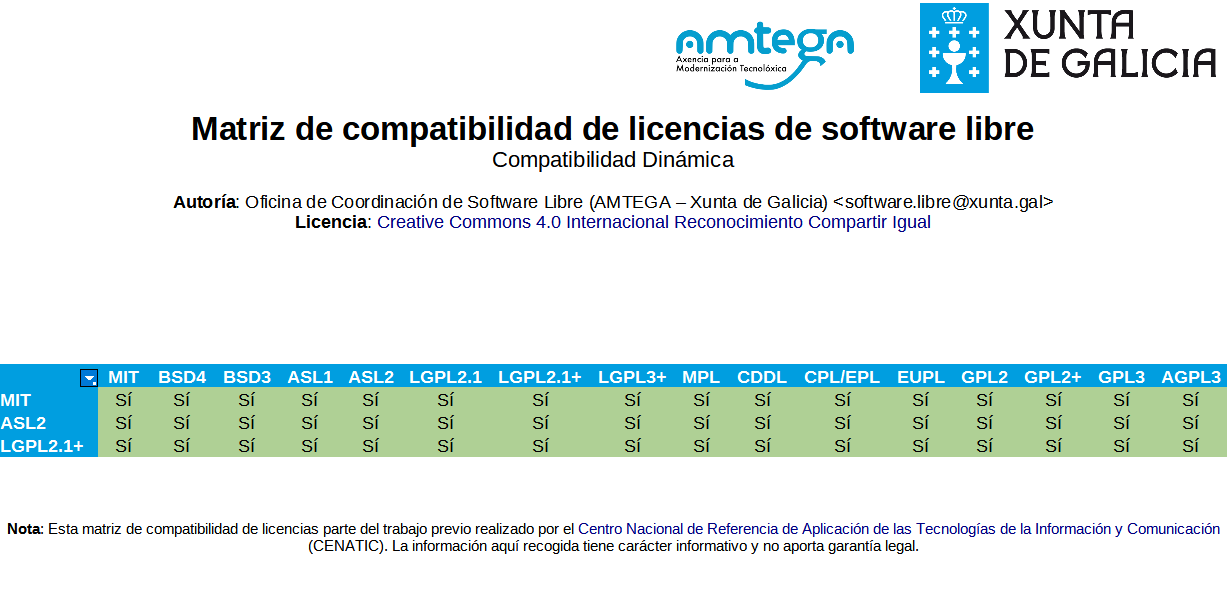
\includegraphics[width=\textwidth]{imagenes/MatrizCompatibilidadDinamica.png}
		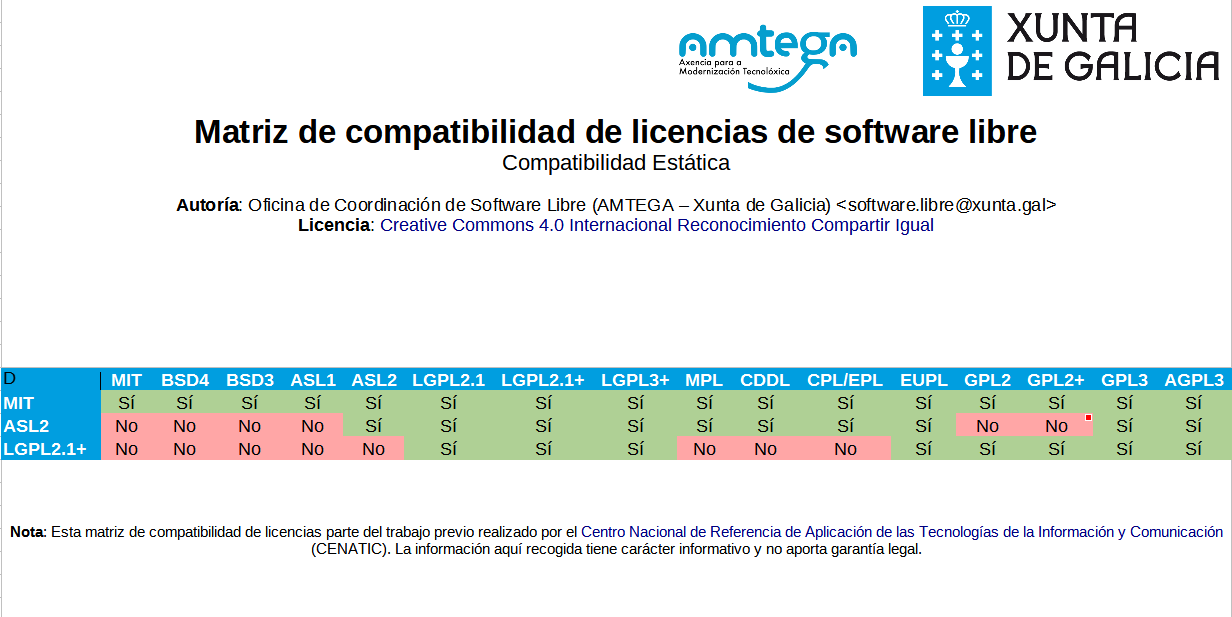
\includegraphics[width=\textwidth]{imagenes/MatrizCompatibilidadEstatica.png}
		\caption{Matriz de compatibilidad de licencias de Software Libre con respecto a licencias Apache 2.0 (ASL2), LGPL 2.1 o superior (LGPL2.1+), y MIT. Matriz extraída de \cite{matriz-licencias}.}
		\label{fig:matrices-comp}
	\end{figure}
\end{center}

A raíz de observar las matrices en la figura \ref{fig:matrices-comp} , tanto la dinámica como la estática, nos quedaríamos con el siguiente listado de candidatos, los cuales listamos anteriormente en la sección \ref{gpl-license-types}:
\begin{itemize}
	\item Lesser GNU Public License 2.1 (con posibilidad de permitir actualizarse a versiones posteriores)
	\item Lesser GNU Public License 3 (con posibilidad de permitir actualizarse a versiones posteriores)
	\item European Union Public License
	\item GNU Public License 3
	\item Affero GNU Public License 3
\end{itemize}

Teniendo en cuenta que las posibilidades de Arcadia se pueden extender a la red gracias a las acciones de Rasa y su posible extensión a un servicio cliente-servidor donde la fuente de conocimiento residiera en un ordenador remoto y el resto de la implementación se quedaría del lado de nuestro ordenador, se opta finalmente por aplicar una licencia AGPL3, la cual se añade al repositorio junto al resto de la documentación.

\begin{table}[H]
	\centering
	\begin{tabularx}{\textwidth}{|>{\columncolor{mintgreen}}c>{\columncolor{mintgreen}}X|}
		\hline
		
\includegraphics[width=30pt]{imagenes/Tarea_completada.png} & Con ello, cumplimos los Objetivos \textbf{O-IA 6.} (Analizar las distintas licencias que se ofrecen y las compatibilidades entre éstas para elegir la idónea para la aplicación resultante.) \\
		\hline
	\end{tabularx}
\end{table}

\subsection{Otros desarrollos que no se han podido completar}
\label{sect:unfinished-dev}
Aparte de lo que se ha realizado para resolver los hitos del proyecto, se han intentado hacer algunas mejoras para facilitar el desarrollo o introducir nuevas funcionalidades, pero han quedado sin éxito tras buscar e investigar sin pdoer conseguir hacer arreglos. Pasamos a listar algunos de ellos:
\begin{itemize}
	\item \textbf{Docker para desarrollo:} Se ha intentado desarrollar un sistema de dos contenedores que hagan ejecutar una instancia de Rasa y otra de nuestro asistente, conectados por una red entre ambos contenedores, con el objetivo de simplificar la ejecución. Al intentar realizarlo, nos hemos encontrado con que al usar las imágenes oficiales del sistema de Chatbot, nos da un error de permisos que no tiene documentada la solución. Tras intentar hacer cambios para que lo aceptara sin éxito, se ha optado por desistir.
	\item \textbf{Segundo hilo para algunas ejecuciones:} Hay cuestiones que precisarían una tarea que se ejecute a la vez que nuestro hilo principal, como puede ser escuchar la radio. Sin embargo, en este momento no se ha conseguido ejecutar un nuevo hilo para estas cuestiones. Se tratará de realizar en un posterior trabajo, permitiendo así la concurrencia y/o paralelismo de las tareas que influyen en Arcadia.
	\item \textbf{Versión para Raspberry Pi}: Si bien sería una buena idea, ya que se podría tener una versión compacta como un prototipo del tamaño de un aparato similar a los competidores con Alexa \cite{alexa} y Echo \cite{echo}, debido a que los contenedores de Docker no están listos, se ha optado por no hacer desarrollos enfocados en la arquitectura ARM que usa esta placa de desarrollo.
\end{itemize}



	% Presupuesto

	% Conclusiones
	\newpage 
	\chapter{Conclusiones y trabajos futuros}

\noindent\fbox{
	\parbox{\textwidth}{
		En este último capítulo se discutirán tópicos que han podido surgir durante el transcurso del Trabajo, posibles mejoras que podrían implementarse en el futuro, qué se ha aplicado en las diferentes asignaturas del Grado y qué se ha aprendido durante el camino que pueda aplicarse en la vida tras esta etapa de aprendizaje.
	}
}
\newline

\section{El proceso de desarrollo en retrospectiva}
Durante el desarrollo de este proyecto se ha podido realizar algunas acciones y cómo han influido a la hora de crear el Software. A modo de retrospectiva de los Sprints del proyecto, hablaremos de esas actuaciones.

\subsection{Lo que ha funcionado}
\begin{itemize}
	\item La \textbf{documentación} de los proyectos que lo componen: Gracias a que los proyectos tienen mucho soporte detrás, se puede encontrar cualquier tópico que se necesite para el desarrollo del programa.
	\item La \textbf{granularidad} de las tareas: Al dedicarse un tiempo a separar el desarrollo del proyecto en los componentes y cada componente en tareas para integrar ese componente al proyecto, la codificación ha sido bastante pautada y de seguimiento fácil.
\end{itemize}
\subsection{Lo que ha funcionado... más o menos}
\begin{itemize}
	\item La realización de \textbf{pruebas}: Las pruebas han sido una parte fundamental del desarrollo para encontrar y tratar de encontrar errores. Si bien al principio se han hecho pruebas unitarias para ir validando la integración de los componentes, una vez que estaba todo unido se tuvieron que pasar a pruebas de campo (como pruebas de concepto o pruebas beta) que posiblemente no se puedan replicar exactamente.
	\item Aplicación de \textbf{SCRUM} para una persona: Las metodologías ágiles tratan de hacer que el desarrollo en equipo sea más dinámico, aunque para una persona la mayoría de las herramientas de ese método de trabajo quizás no sean muy útiles. No obstante, la parte más básica ha permitido entender mejor las tareas y cuándo realizarlas; y poder entender cómo mejorar tras cada parte para continuar trabajando así, o realizando cambios en el flujo de trabajo.
\end{itemize}
\subsection{Lo que no ha funcionado}
\begin{itemize}
	\item Los \textbf{tiempos}: El tiempo pensado de desarrollo que se comentó en la Figura \ref{fig:gantt} no se ha ajustado a la realidad, concentrando el desarrollo entre finales de Abril y la primera semana de Junio. Ello ha dado a las cuestiones que se detallarán en el siguiente apartado.
\end{itemize}
\subsection{Tiempo estimado vs. Tiempo real}
Con los tiempos reales se ha confeccionado este nuevo Diagrama de Gantt (véase Figura \ref{fig:gantt_tr}), donde las mayores diferencias con el anterior (Figura \ref{fig:gantt}) radican en:
\begin{itemize}
	\item El Sprint 0 ha sido prolongado, abarcando la mayor parte del tiempo estimado para el desarrollo. Si bien ese tiempo parece mucho, realmente se ha trabajado en ello unas 3 semanas (2 de realización más 1 para las correcciones propuestas por el Profesor encargado de la supervisión del Trabajo Final de Grado).
	\item A raíz de la premisa anterior, los demás Sprints han sido recortados aunque el tiempo dedicado ha sido constante, si bien había tareas que no han necesitado tanto tiempo de codificación.
	\item Se han añadido dos nuevas tareas en el Sprint 4:
	\begin{itemize}
		\item Crear un archivo de Contribución.
		\item Crear plantillas para los Issues de GitHub.
	\end{itemize}
	
\end{itemize}

\begin{figure}[h]
	\centering
	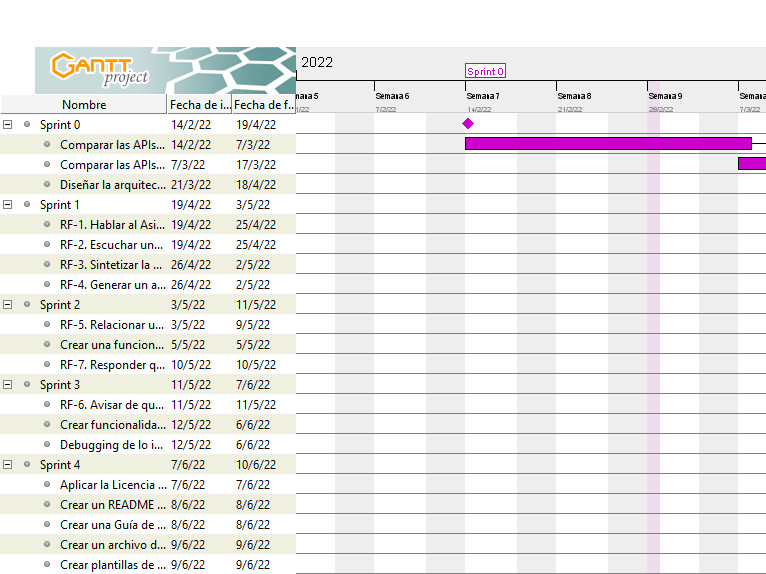
\includegraphics[width=\textwidth]{imagenes/GanttTR3.png} \\
	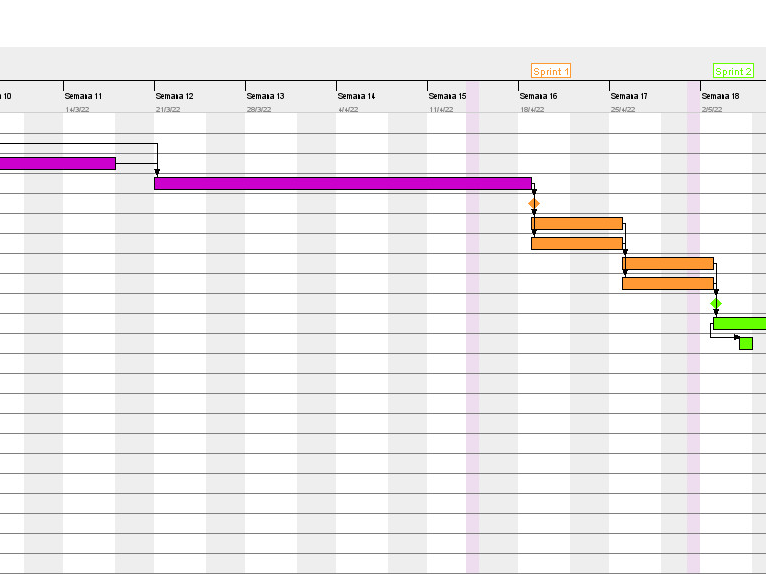
\includegraphics[width=0.48\textwidth]{imagenes/GanttTR2.png}
	\includegraphics[width=0.48\textwidth]{imagenes/GanttTR1.png}
	\caption[Diagrama de Gantt]{Diagrama de Gantt del proyecto con los tiempos reales. De elaboración propia, generado con GanttProject.}
	\label{fig:gantt_tr}
\end{figure}

\subsection{Cumplimiento de los objetivos}

Durante el desarrollo se han tratado de cubrir los objetivos tanto de Investigación y Aprendizaje como de Diseño y Desarrollo.

\subsubsection{Objetivos de Investigación y Aprendizaje}

\begin{enumerate}[O-{IA}.1 -]
	\item Entender el funcionamiento de los Asistentes de Voz. (100\% completado.)
	\item Analizar el panorama del campo de los Asistentes de Voz y los avances que se han realizado.(100\% completado.)
	\item Analizar desde un punto de vista competitivo las prestaciones que ofrecen otras alternativas propietarias y libres (si las hay). (100\% completado.)
	\item Sintetizar los posibles componentes que conforman un Asistente de Voz y la escalabilidad de cada uno de ellos. (100\% completado.)
	\item Entender el impacto del software propietario y sus alternativas libres o de Código Abierto. (100\% completado.)
	\item Analizar las distintas licencias que se ofrecen y las compatibilidades entre éstas para elegir la idónea para la aplicación resultante. (100\% completado.)
	\item Leer sobre aquellos estándares y convenciones para facilitar la compartición y liberación del proyecto (por ejemplo. Códigos de conducta, Guías de contribución) (100\% completado.)
	\item Analizar el impacto que los descubrimientos en los Asistentes de Voz pueden producir en la Sociedad de la Información. (100\% completado.)
\end{enumerate}

\subsubsection{Objetivos de Diseño y Desarrollo}

\begin{enumerate}[O-DD.1 -]
	\item Diseñar personas y casos de uso en los que el software podría presentar algún problema con tal de buscar soluciones o limitaciones. (100\% completado.)
	\item Diseñar las clases que albergarán los componentes de un Asistente de Voz, su interacción con los periféricos de Entrada/Salida y con aquellas APIs externas que se requieran para el funcionamiento básico del programa. (100\% completado.)
	\item Idear una vía para escalar el número de posibles frases e interacciones que pueda reconocer el proyecto. (100\% completado.)
	\item Planear la arquitectura del proyecto resultante, siguiendo las buenas prácticas del Desarrollo de Software. (100\% completado.)
	\item Con base a la arquitectura, codificar lo necesario para la implementación de la aplicación. (100\% completado.)
	\item Redactar documentación referida a la arquitectura del proyecto para su posterior mantenimiento y escalabilidad. (100\% completado.)
	
\end{enumerate}


\section{¿Y ahora qué? Posibles trabajos y mejoras en el futuro.}
Si bien el proyecto puede ser usable y se le podría dar el \textit{status} de Producto Mínimo Viable, hay algunas cuestiones que facilitarían el uso y desarrollo de Arcadia para otros desarrolladores, o son tareas que no se han podido realizar durante el desarrollo. Listaremos algunos de ellos:

\begin{itemize}
	\item Los listados en la sección \ref{sect:unfinished-dev}, a los que estaría bien echar otro vistazo y acotarlos desde otro punto de vista.
	\item Añadir elementos de Integración Continua y Despliegue Continuo. Esto podría ayudar a automatizar los procesos monótonos como el formato del código, o ayudar a otros desarrolladores a subir su código según los estándares. Para ello, se estudiará sobre el tema y se tratará de integrar estos procesos a través de la forja usando GitHub Actions.
	\item Mejorar la documentación, tanto la calidad de este (añadiendo guías para realizar algunos cambios, por ejemplo), como el formato de presentación (usando GitHub Pages  o creando una documentación en PDF, como alternativas).
\end{itemize}

\section{Arcadia, los Asistentes Virtuales y el impacto en la sociedad}
Como se comentó en la Introducción, estamos en una época donde las nuevas tecnologías tratan de ser explotadas rápidamente, conectando a las personas y la información que se puede generar de ellas para propósitos variados. Además se habló de cómo las empresas protegían sus intereses y las protecciones que el estado les ofrece, y cómo el Software Libre y el Software de Código Abierto pueden resultar como alternativas de tal modelo proteccionista.

Los Asistentes Virtuales, como ejemplo de tecnología recientemente puesto a explotación por grandes empresas, son a veces objeto de sospechas por parte del público general y pueden causar cierto sentimiento de vigilancia. Aún así, la mayoría que usa ese tipo de aplicaciones tiende también a antropomorfizar la voz \cite{va-antromorfismos} que sale del altavoz, haciéndolo familiar. De esta forma, nos encontramos con una especie de limbo ético en este campo, ya que nos encontramos entre la usabilidad del producto, la demanda del público, y el interés de terceros por saber lo que una persona quiere o necesita.

Para resolver este problema, como hemos podido ver durante el transcurso de este Trabajo, se puede volver a pensar en estos sistemas con otros prismas. Uno de estos, el cual hemos explorado en detalle en este proyecto, es usar el Software Abierto y Libre y crear un núcleo que contenga esos proyectos, que se pueda adaptar a otras implementaciones y que todo lo que concierne a la aplicación se pueda consultar en cualquier momento gracias a que el código es público.

Teniendo en cuenta esta base, se ha tratado de conseguir que Arcadia cumpla con estas premisas, y que además sea abierto para cualquiera para hacer los cambios que desee, o reportar cualquier incidencia. De esta manera, la comunidad de desarrolladores y curiosos en la materia podrían ayudar a mantener la responsabilidad ética de este proyecto.

Aún así, se podrían dar algunas cuestiones que romperían los principios del proyecto. Al ser abierto, cualquiera podría hacer los cambios que desee, incluyendo la combinación del núcleo con un componente privativo, haciendo que esa versión alternativa no sea totalmente libre. Aún así, debido a que nuestro software está regido por la licencia AGPLv3 \cite{gplv3}, tiene en regencia las 4 Libertades \cite{fsf-philosophy}, de las cuales las 3 últimas permiten esa copia y redistribución.

Por otra parte, al ser un núcleo del que se conectan otros proyectos, podemos tener como preocupación el soporte de esos componentes. Puede que con el tiempo, esos componentes pasen a ser obsoletos y/o dejen de usar licencias compatibles con la que tiene Arcadia. De todas formas, gracias a la forma para realizar las adaptaciones, podemos introducir otros proyectos al software, formando así muchos sabores y versiones de esta aplicación, y pudiendo paliar así el problema.

\section{El proceso de aprendizaje y la distribución del conocimiento}
Desde la redacción de la primera página, se ha realizado un proceso de aprendizaje pautado sobre los conceptos a desarrollar y en qué fundamentos se basaban las tecnologías de los componentes a usar, para después buscar alternativas que utilizar en base a los intereses y restricciones del proyecto, y finalmente evaluarlos y usarlos para la codificación de Arcadia. En el proceso se han consultado multitud de portales web, papers y algún que otro manual o portal de documentación. En especial, se podría destacar la documentación de Rasa, ya que era muy completa y describía cualquier detalle relacionado con el entorno, con un portal de documentación web y muchas videoguías que permitieron probar el software y aprender a hacer funcionalidades sin mucha dificultad.

Aunque se ha querido explicar todo en esta Memoria, puede que haya un público muy reducido que acabe leyéndola (aunque esté disponible en GitHub), por lo que se ha querido también exponer este aprendizaje a cualquier interesado. De esta manera se realizó una charla en Marzo de 2022 hablando sobre los componentes de un Asistente Virtual y experimentando su funcionamiento. A pesar de los errores técnicos y la inexperiencia dando este tipo de exposiciones, los asistentes llegaron a comentar que les interesó mucho.



\section{Unas últimas palabras: Valoración personal}
Para esta sección, permitidme que pase de la tercera a la primera persona para poder contar las sensaciones y valoraciones que tengo en estas últimas líneas de la Memoria.

Hacer este trabajo ha sido la mezcla de un interés que tenía latente desde la mitad del transcurso de la carrera; junto con la necesidad de hacer un Trabajo Final de Grado que pudiera ser interesante y que permitiera plasmar todo lo aprendido durante esta etapa y cerrarla con satisfacción.

Han pasado aproximadamente 7 meses desde la primera reunión con el Tutor del TFG donde se discutieron las ideas escritas en un correo que recogía la propuesta, y gracias a lo cual se pudo definir todo el rumbo que llevaría este proyecto. Desde entonces, el flujo de correos y reuniones para revisar cómo iba esta aplicación ha sido llevadero y ameno, donde las correcciones y apreciaciones me servían para poder mejorar la redacción y los contenidos que quería exponer en este escrito. 

Desarrollar a Arcadia ha sido una pequeña odisea que ha requerido un tiempo considerable, pero se ha podido conllevar bien con el resto de tareas académicas, profesionales y personales. También me ha servido de desafío personal para ser constante y mejorar y aplicar todo lo acontecido en la etapa universitaria.

Si bien este proyecto no deja de ser un Trabajo Final de Grado, desearía continuar con el desarrollo de este. Quizás como hobby, como distracción o como manera de aplicar nuevas tecnologías relacionadas. 

Aprender por cuenta de uno mismo tiende a ser un paso natural en este tipo de trabajos, pero a pesar de ello siempre viene bien toda ayuda (sea a través de material o hablando con alguien que sepa de alguno de los temas que rodeen lo que se quiere saber). Por mi parte, sentía también que una parte de aprender es enseñar a otros que les interesen, dando pie a un ciclo virtuoso.

En definitiva, y dando punto y final a esta Memoria, ha sido un TFG que he disfrutado en la confección y donde me he sentido bien asesorado y capacitado para cumplir con lo descrito, cosa que puede que continúe realizando y enseñando en el futuro.


	% Trabajos futuros


	
	\newpage
	\bibliography{bibliografia}
	\bibliographystyle{plain}
	
\end{document}

